\documentclass[twoside]{book}

% Packages required by doxygen
\usepackage{fixltx2e}
\usepackage{calc}
\usepackage{doxygen}
\usepackage[export]{adjustbox} % also loads graphicx
\usepackage{graphicx}
\usepackage[utf8]{inputenc}
\usepackage{makeidx}
\usepackage{multicol}
\usepackage{multirow}
\PassOptionsToPackage{warn}{textcomp}
\usepackage{textcomp}
\usepackage[nointegrals]{wasysym}
\usepackage[table]{xcolor}

% Font selection
\usepackage[T1]{fontenc}
\usepackage[scaled=.90]{helvet}
\usepackage{courier}
\usepackage{amssymb}
\usepackage{sectsty}
\renewcommand{\familydefault}{\sfdefault}
\allsectionsfont{%
  \fontseries{bc}\selectfont%
  \color{darkgray}%
}
\renewcommand{\DoxyLabelFont}{%
  \fontseries{bc}\selectfont%
  \color{darkgray}%
}
\newcommand{\+}{\discretionary{\mbox{\scriptsize$\hookleftarrow$}}{}{}}

% Page & text layout
\usepackage{geometry}
\geometry{%
  a4paper,%
  top=2.5cm,%
  bottom=2.5cm,%
  left=2.5cm,%
  right=2.5cm%
}
\tolerance=750
\hfuzz=15pt
\hbadness=750
\setlength{\emergencystretch}{15pt}
\setlength{\parindent}{0cm}
\setlength{\parskip}{3ex plus 2ex minus 2ex}
\makeatletter
\renewcommand{\paragraph}{%
  \@startsection{paragraph}{4}{0ex}{-1.0ex}{1.0ex}{%
    \normalfont\normalsize\bfseries\SS@parafont%
  }%
}
\renewcommand{\subparagraph}{%
  \@startsection{subparagraph}{5}{0ex}{-1.0ex}{1.0ex}{%
    \normalfont\normalsize\bfseries\SS@subparafont%
  }%
}
\makeatother

% Headers & footers
\usepackage{fancyhdr}
\pagestyle{fancyplain}
\fancyhead[LE]{\fancyplain{}{\bfseries\thepage}}
\fancyhead[CE]{\fancyplain{}{}}
\fancyhead[RE]{\fancyplain{}{\bfseries\leftmark}}
\fancyhead[LO]{\fancyplain{}{\bfseries\rightmark}}
\fancyhead[CO]{\fancyplain{}{}}
\fancyhead[RO]{\fancyplain{}{\bfseries\thepage}}
\fancyfoot[LE]{\fancyplain{}{}}
\fancyfoot[CE]{\fancyplain{}{}}
\fancyfoot[RE]{\fancyplain{}{\bfseries\scriptsize Generated by Doxygen }}
\fancyfoot[LO]{\fancyplain{}{\bfseries\scriptsize Generated by Doxygen }}
\fancyfoot[CO]{\fancyplain{}{}}
\fancyfoot[RO]{\fancyplain{}{}}
\renewcommand{\footrulewidth}{0.4pt}
\renewcommand{\chaptermark}[1]{%
  \markboth{#1}{}%
}
\renewcommand{\sectionmark}[1]{%
  \markright{\thesection\ #1}%
}

% Indices & bibliography
\usepackage{natbib}
\usepackage[titles]{tocloft}
\setcounter{tocdepth}{3}
\setcounter{secnumdepth}{5}
\makeindex

% Hyperlinks (required, but should be loaded last)
\usepackage{ifpdf}
\ifpdf
  \usepackage[pdftex,pagebackref=true]{hyperref}
\else
  \usepackage[ps2pdf,pagebackref=true]{hyperref}
\fi
\hypersetup{%
  colorlinks=true,%
  linkcolor=blue,%
  citecolor=blue,%
  unicode%
}

% Custom commands
\newcommand{\clearemptydoublepage}{%
  \newpage{\pagestyle{empty}\cleardoublepage}%
}

\usepackage{caption}
\captionsetup{labelsep=space,justification=centering,font={bf},singlelinecheck=off,skip=4pt,position=top}

%===== C O N T E N T S =====

\begin{document}

% Titlepage & ToC
\hypersetup{pageanchor=false,
             bookmarksnumbered=true,
             pdfencoding=unicode
            }
\pagenumbering{alph}
\begin{titlepage}
\vspace*{7cm}
\begin{center}%
{\Large trifinger\+\_\+simulation }\\
\vspace*{1cm}
{\large Generated by Doxygen 1.8.13}\\
\end{center}
\end{titlepage}
\clearemptydoublepage
\pagenumbering{roman}
\tableofcontents
\clearemptydoublepage
\pagenumbering{arabic}
\hypersetup{pageanchor=true}

%--- Begin generated contents ---
\chapter{Tri\+Finger Robot Simulation}
\label{md_README}
\Hypertarget{md_README}
This package provides a real-\/time A\+PI for communication with the motor control board and the Opto\+Force sensor via C\+AN.

A description of the C\+AN protocol that is implemented by this library can be found on Confluence\+: \href{https://atlas.is.localnet/confluence/display/AMDW/BLMC+-+CAN+Interface}{\tt https\+://atlas.\+is.\+localnet/confluence/display/\+A\+M\+D\+W/\+B\+L\+M\+C+-\/+\+C\+A\+N+\+Interface}

This package contains a executable blmc\+\_\+can\+\_\+demo, that shows how to use the library.

\subsection*{Dependencies and other Requirements }

Supports (tested) Ubuntu patched with R\+T-\/preempt. Supports (experimental) Mac OS , Ubuntu patched with Xenomai

(see\+: \href{https://github.com/machines-in-motion/real_time_tools}{\tt https\+://github.\+com/machines-\/in-\/motion/real\+\_\+time\+\_\+tools})

A real-\/time C\+AN driver has to be loaded and the interface to be set up. This can be done with the script {\ttfamily start\+\_\+rtcan} that is included in the xenomai-\/core repository (\href{https://git-amd.tuebingen.mpg.de/amd-clmc/xenomai-core}{\tt https\+://git-\/amd.\+tuebingen.\+mpg.\+de/amd-\/clmc/xenomai-\/core}).

Note that the board has to run a program that implements the same C\+AN protocol. At the time of writing this R\+E\+A\+D\+ME, this is only the case for dual\+\_\+motor\+\_\+torque\+\_\+ctrl.

\subsection*{Documentation }

The code is well documented with Doxygen comments. To generate a H\+T\+ML documentation, build with \begin{DoxyVerb}catkin_make install -DBUILD_DOCUMENTATION=ON
\end{DoxyVerb}


Documentations will be in $<$\+Workspace$>$/install/share/

\subsection*{Authors }


\begin{DoxyItemize}
\item Felix Widmaier
\item Manuel Wuethrich
\item Maximilien Naveau
\item Steve Heim
\item Diego Agudelo
\item Julian Viereck
\end{DoxyItemize}

\subsection*{Copyrights }

Copyright(c) 2018-\/2019 Max Planck Gesellschaft, New York University

\subsection*{License }

B\+SD 3-\/\+Clause License 
\chapter{Hierarchical Index}
\section{Class Hierarchy}
This inheritance list is sorted roughly, but not completely, alphabetically\+:\begin{DoxyCompactList}
\item \contentsline{section}{trifinger\+\_\+simulation.\+action.\+Action}{\pageref{classtrifinger__simulation_1_1action_1_1Action}}{}
\item \contentsline{section}{trifinger\+\_\+simulation.\+collision\+\_\+objects.\+Block}{\pageref{classtrifinger__simulation_1_1collision__objects_1_1Block}}{}
\item \contentsline{section}{trifinger\+\_\+simulation.\+trifinger\+\_\+platform.\+Camera\+Observation}{\pageref{classtrifinger__simulation_1_1trifinger__platform_1_1CameraObservation}}{}
\item \contentsline{section}{trifinger\+\_\+simulation.\+visual\+\_\+objects.\+Cube\+Marker}{\pageref{classtrifinger__simulation_1_1visual__objects_1_1CubeMarker}}{}
\item \contentsline{section}{trifinger\+\_\+simulation.\+gym\+\_\+wrapper.\+data\+\_\+logger.\+Data\+Logger}{\pageref{classtrifinger__simulation_1_1gym__wrapper_1_1data__logger_1_1DataLogger}}{}
\item Env\begin{DoxyCompactList}
\item \contentsline{section}{example\+\_\+pushing\+\_\+training\+\_\+env.\+Example\+Pushing\+Training\+Env}{\pageref{classexample__pushing__training__env_1_1ExamplePushingTrainingEnv}}{}
\item \contentsline{section}{trifinger\+\_\+simulation.\+gym\+\_\+wrapper.\+envs.\+trifinger\+\_\+push.\+Tri\+Finger\+Push}{\pageref{classtrifinger__simulation_1_1gym__wrapper_1_1envs_1_1trifinger__push_1_1TriFingerPush}}{}
\item \contentsline{section}{trifinger\+\_\+simulation.\+gym\+\_\+wrapper.\+envs.\+trifinger\+\_\+reach.\+Tri\+Finger\+Reach}{\pageref{classtrifinger__simulation_1_1gym__wrapper_1_1envs_1_1trifinger__reach_1_1TriFingerReach}}{}
\end{DoxyCompactList}
\item \contentsline{section}{trifinger\+\_\+simulation.\+gym\+\_\+wrapper.\+data\+\_\+logger.\+Episode\+Data}{\pageref{classtrifinger__simulation_1_1gym__wrapper_1_1data__logger_1_1EpisodeData}}{}
\item Exception\begin{DoxyCompactList}
\item \contentsline{section}{trifinger\+\_\+simulation.\+tasks.\+move\+\_\+cube.\+Invalid\+Goal\+Error}{\pageref{classtrifinger__simulation_1_1tasks_1_1move__cube_1_1InvalidGoalError}}{}
\end{DoxyCompactList}
\item \contentsline{section}{trifinger\+\_\+simulation.\+gym\+\_\+wrapper.\+finger\+\_\+spaces.\+Finger\+Spaces}{\pageref{classtrifinger__simulation_1_1gym__wrapper_1_1finger__spaces_1_1FingerSpaces}}{}
\item \contentsline{section}{trifinger\+\_\+simulation.\+visual\+\_\+objects.\+Marker}{\pageref{classtrifinger__simulation_1_1visual__objects_1_1Marker}}{}
\item Named\+Tuple\begin{DoxyCompactList}
\item \contentsline{section}{run\+\_\+evaluate\+\_\+policy\+\_\+all\+\_\+levels.\+Test\+Sample}{\pageref{classrun__evaluate__policy__all__levels_1_1TestSample}}{}
\item \contentsline{section}{run\+\_\+replay\+\_\+all\+\_\+levels.\+Test\+Sample}{\pageref{classrun__replay__all__levels_1_1TestSample}}{}
\item \contentsline{section}{trifinger\+\_\+simulation.\+finger\+\_\+types\+\_\+data.\+Finger\+Types\+Data\+Format}{\pageref{classtrifinger__simulation_1_1finger__types__data_1_1FingerTypesDataFormat}}{}
\end{DoxyCompactList}
\item object\begin{DoxyCompactList}
\item \contentsline{section}{trifinger\+\_\+simulation.\+camera.\+Camera}{\pageref{classtrifinger__simulation_1_1camera_1_1Camera}}{}
\end{DoxyCompactList}
\item \contentsline{section}{trifinger\+\_\+simulation.\+trifinger\+\_\+platform.\+Object\+Pose}{\pageref{classtrifinger__simulation_1_1trifinger__platform_1_1ObjectPose}}{}
\item \contentsline{section}{trifinger\+\_\+simulation.\+observation.\+Observation}{\pageref{classtrifinger__simulation_1_1observation_1_1Observation}}{}
\item Observation\+Wrapper\begin{DoxyCompactList}
\item \contentsline{section}{example\+\_\+pushing\+\_\+training\+\_\+env.\+Flat\+Observation\+Wrapper}{\pageref{classexample__pushing__training__env_1_1FlatObservationWrapper}}{}
\end{DoxyCompactList}
\item \contentsline{section}{trifinger\+\_\+simulation.\+pinocchio\+\_\+utils.\+Pinocchio\+Utils}{\pageref{classtrifinger__simulation_1_1pinocchio__utils_1_1PinocchioUtils}}{}
\item \contentsline{section}{trifinger\+\_\+simulation.\+tasks.\+move\+\_\+cube.\+Pose}{\pageref{classtrifinger__simulation_1_1tasks_1_1move__cube_1_1Pose}}{}
\item \contentsline{section}{evaluate\+\_\+policy.\+P\+P\+O\+Policy}{\pageref{classevaluate__policy_1_1PPOPolicy}}{}
\item \contentsline{section}{evaluate\+\_\+policy.\+Random\+Policy}{\pageref{classevaluate__policy_1_1RandomPolicy}}{}
\item \contentsline{section}{demo\+\_\+random\+\_\+policy.\+Random\+Policy}{\pageref{classdemo__random__policy_1_1RandomPolicy}}{}
\item \contentsline{section}{trifinger\+\_\+simulation.\+real\+\_\+finger.\+Real\+Finger}{\pageref{classtrifinger__simulation_1_1real__finger_1_1RealFinger}}{}
\item Robot\+Driver\begin{DoxyCompactList}
\item \contentsline{section}{trifinger\+\_\+simulation\+:\+:Base\+Py\+Bullet\+Finger\+Driver$<$ robot\+\_\+interfaces\+:\+:Mono\+Finger\+Types\+:\+:Action, robot\+\_\+interfaces\+:\+:Mono\+Finger\+Types\+:\+:Observation $>$}{\pageref{classtrifinger__simulation_1_1BasePyBulletFingerDriver}}{}
\begin{DoxyCompactList}
\item \contentsline{section}{trifinger\+\_\+simulation\+:\+:Py\+Bullet\+Single\+Finger\+Driver}{\pageref{classtrifinger__simulation_1_1PyBulletSingleFingerDriver}}{}
\end{DoxyCompactList}
\item \contentsline{section}{trifinger\+\_\+simulation\+:\+:Base\+Py\+Bullet\+Finger\+Driver$<$ robot\+\_\+interfaces\+:\+:Tri\+Finger\+Types\+:\+:Action, robot\+\_\+interfaces\+:\+:Tri\+Finger\+Types\+:\+:Observation $>$}{\pageref{classtrifinger__simulation_1_1BasePyBulletFingerDriver}}{}
\begin{DoxyCompactList}
\item \contentsline{section}{trifinger\+\_\+simulation\+:\+:Py\+Bullet\+Tri\+Finger\+Driver}{\pageref{classtrifinger__simulation_1_1PyBulletTriFingerDriver}}{}
\end{DoxyCompactList}
\item \contentsline{section}{trifinger\+\_\+simulation\+:\+:Base\+Py\+Bullet\+Finger\+Driver$<$ Action, Observation $>$}{\pageref{classtrifinger__simulation_1_1BasePyBulletFingerDriver}}{}
\end{DoxyCompactList}
\item \contentsline{section}{trifinger\+\_\+simulation.\+sim\+\_\+finger.\+Sim\+Finger}{\pageref{classtrifinger__simulation_1_1sim__finger_1_1SimFinger}}{}
\item \contentsline{section}{trifinger\+\_\+simulation.\+trifinger\+\_\+platform.\+Tri\+Camera\+Observation}{\pageref{classtrifinger__simulation_1_1trifinger__platform_1_1TriCameraObservation}}{}
\item \contentsline{section}{trifinger\+\_\+simulation.\+camera.\+Tri\+Finger\+Cameras}{\pageref{classtrifinger__simulation_1_1camera_1_1TriFingerCameras}}{}
\item \contentsline{section}{trifinger\+\_\+simulation.\+trifinger\+\_\+platform.\+Tri\+Finger\+Platform}{\pageref{classtrifinger__simulation_1_1trifinger__platform_1_1TriFingerPlatform}}{}
\end{DoxyCompactList}

\chapter{Class Index}
\section{Class List}
Here are the classes, structs, unions and interfaces with brief descriptions\+:\begin{DoxyCompactList}
\item\contentsline{section}{\hyperlink{classrobot__properties__solo_1_1quadruped12wrapper_1_1Quadruped12Robot}{robot\+\_\+properties\+\_\+solo.\+quadruped12wrapper.\+Quadruped12\+Robot} }{\pageref{classrobot__properties__solo_1_1quadruped12wrapper_1_1Quadruped12Robot}}{}
\item\contentsline{section}{\hyperlink{classrobot__properties__solo_1_1config_1_1Solo12Config}{robot\+\_\+properties\+\_\+solo.\+config.\+Solo12\+Config} }{\pageref{classrobot__properties__solo_1_1config_1_1Solo12Config}}{}
\item\contentsline{section}{\hyperlink{classrobot__properties__solo_1_1solo8wrapper_1_1Solo8Robot}{robot\+\_\+properties\+\_\+solo.\+solo8wrapper.\+Solo8\+Robot} }{\pageref{classrobot__properties__solo_1_1solo8wrapper_1_1Solo8Robot}}{}
\item\contentsline{section}{\hyperlink{classrobot__properties__solo_1_1config_1_1SoloAbstract}{robot\+\_\+properties\+\_\+solo.\+config.\+Solo\+Abstract} \\*Abstract class used for all Solo robots }{\pageref{classrobot__properties__solo_1_1config_1_1SoloAbstract}}{}
\item\contentsline{section}{\hyperlink{classrobot__properties__solo_1_1config_1_1SoloConfig}{robot\+\_\+properties\+\_\+solo.\+config.\+Solo\+Config} }{\pageref{classrobot__properties__solo_1_1config_1_1SoloConfig}}{}
\end{DoxyCompactList}

\chapter{File Index}
\section{File List}
Here is a list of all documented files with brief descriptions\+:\begin{DoxyCompactList}
\item\contentsline{section}{include/\hyperlink{AtiFTSensor_8h}{Ati\+F\+T\+Sensor.\+h} }{\pageref{AtiFTSensor_8h}}{}
\end{DoxyCompactList}

\chapter{Class Documentation}
\hypertarget{classtrifinger__simulation_1_1action_1_1Action}{}\section{trifinger\+\_\+simulation.\+action.\+Action Class Reference}
\label{classtrifinger__simulation_1_1action_1_1Action}\index{trifinger\+\_\+simulation.\+action.\+Action@{trifinger\+\_\+simulation.\+action.\+Action}}


Robot action.  


\subsection*{Public Member Functions}
\begin{DoxyCompactItemize}
\item 
def \hyperlink{classtrifinger__simulation_1_1action_1_1Action_a8cf3247a4080f46bc05c62ba66ec8016}{\+\_\+\+\_\+init\+\_\+\+\_\+} (self, torque, position, kp=None, kd=None)
\begin{DoxyCompactList}\small\item\em Initialize. \end{DoxyCompactList}\end{DoxyCompactItemize}
\subsection*{Public Attributes}
\begin{DoxyCompactItemize}
\item 
\mbox{\Hypertarget{classtrifinger__simulation_1_1action_1_1Action_afa60ba875dbdd6c4903f04760a5c20d9}\label{classtrifinger__simulation_1_1action_1_1Action_afa60ba875dbdd6c4903f04760a5c20d9}} 
{\bfseries torque}
\item 
\mbox{\Hypertarget{classtrifinger__simulation_1_1action_1_1Action_ad5a6eb34bca8a17b78c70df059fa01ff}\label{classtrifinger__simulation_1_1action_1_1Action_ad5a6eb34bca8a17b78c70df059fa01ff}} 
{\bfseries position}
\item 
\mbox{\Hypertarget{classtrifinger__simulation_1_1action_1_1Action_a86037a7a4580aea71607188aeafa7bfd}\label{classtrifinger__simulation_1_1action_1_1Action_a86037a7a4580aea71607188aeafa7bfd}} 
{\bfseries position\+\_\+kp}
\item 
\mbox{\Hypertarget{classtrifinger__simulation_1_1action_1_1Action_ac42443e1e4f0be5c6db4dab6c28417c4}\label{classtrifinger__simulation_1_1action_1_1Action_ac42443e1e4f0be5c6db4dab6c28417c4}} 
{\bfseries position\+\_\+kd}
\end{DoxyCompactItemize}


\subsection{Detailed Description}
Robot action. 

The length of the attributes depends on the robot type. In the following {\ttfamily n\+\_\+joints} is the number of joints and {\ttfamily n\+\_\+fingers} the number of fingers (e.\+g. for the Tri\+Finger robots {\ttfamily n\+\_\+fingers = 3, n\+\_\+joints = 9}).

\begin{DoxyVerb}    torque (array, shape=(n_joints,)):  Torque commands for the joints.
    position (array, shape=(n_joints,)):  Position commands for the joints.
        Set to NaN to disable position control for the corresponding joint.
    kp (array, shape=(n_joints,)):  P-gain for position controller.  Set to
        NaN to use default gain for the corresponding joint.
    kd (array, shape=(n_joints,)):  D-gain for position controller.  Set to
        NaN to use default gain for the corresponding joint.\end{DoxyVerb}
 

\subsection{Constructor \& Destructor Documentation}
\mbox{\Hypertarget{classtrifinger__simulation_1_1action_1_1Action_a8cf3247a4080f46bc05c62ba66ec8016}\label{classtrifinger__simulation_1_1action_1_1Action_a8cf3247a4080f46bc05c62ba66ec8016}} 
\index{trifinger\+\_\+simulation\+::action\+::\+Action@{trifinger\+\_\+simulation\+::action\+::\+Action}!\+\_\+\+\_\+init\+\_\+\+\_\+@{\+\_\+\+\_\+init\+\_\+\+\_\+}}
\index{\+\_\+\+\_\+init\+\_\+\+\_\+@{\+\_\+\+\_\+init\+\_\+\+\_\+}!trifinger\+\_\+simulation\+::action\+::\+Action@{trifinger\+\_\+simulation\+::action\+::\+Action}}
\subsubsection{\texorpdfstring{\+\_\+\+\_\+init\+\_\+\+\_\+()}{\_\_init\_\_()}}
{\footnotesize\ttfamily def trifinger\+\_\+simulation.\+action.\+Action.\+\_\+\+\_\+init\+\_\+\+\_\+ (\begin{DoxyParamCaption}\item[{}]{self,  }\item[{}]{torque,  }\item[{}]{position,  }\item[{}]{kp = {\ttfamily None},  }\item[{}]{kd = {\ttfamily None} }\end{DoxyParamCaption})}



Initialize. 


\begin{DoxyParams}{Parameters}
{\em torque} & See \+:attr\+:{\ttfamily torque}. \\
\hline
{\em position} & See \+:attr\+:{\ttfamily position}. \\
\hline
{\em kp} & See \+:attr\+:{\ttfamily kp}. \\
\hline
{\em kd} & See \+:attr\+:{\ttfamily kd}. \\
\hline
\end{DoxyParams}


The documentation for this class was generated from the following file\+:\begin{DoxyCompactItemize}
\item 
python/trifinger\+\_\+simulation/action.\+py\end{DoxyCompactItemize}

\hypertarget{classtrifinger__simulation_1_1BasePyBulletFingerDriver}{}\section{trifinger\+\_\+simulation\+:\+:Base\+Py\+Bullet\+Finger\+Driver$<$ Action, Observation $>$ Class Template Reference}
\label{classtrifinger__simulation_1_1BasePyBulletFingerDriver}\index{trifinger\+\_\+simulation\+::\+Base\+Py\+Bullet\+Finger\+Driver$<$ Action, Observation $>$@{trifinger\+\_\+simulation\+::\+Base\+Py\+Bullet\+Finger\+Driver$<$ Action, Observation $>$}}


Base driver for py\+Bullet of both single Finger and Tri\+Finger.  




{\ttfamily \#include $<$pybullet\+\_\+driver.\+hpp$>$}



Inheritance diagram for trifinger\+\_\+simulation\+:\+:Base\+Py\+Bullet\+Finger\+Driver$<$ Action, Observation $>$\+:
\nopagebreak
\begin{figure}[H]
\begin{center}
\leavevmode
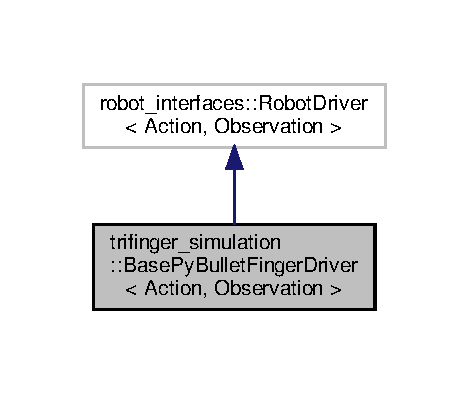
\includegraphics[width=225pt]{classtrifinger__simulation_1_1BasePyBulletFingerDriver__inherit__graph}
\end{center}
\end{figure}


Collaboration diagram for trifinger\+\_\+simulation\+:\+:Base\+Py\+Bullet\+Finger\+Driver$<$ Action, Observation $>$\+:
\nopagebreak
\begin{figure}[H]
\begin{center}
\leavevmode
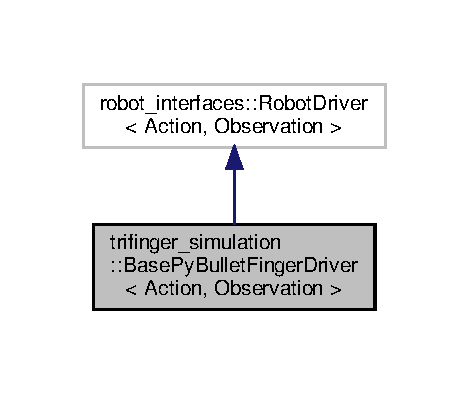
\includegraphics[width=225pt]{classtrifinger__simulation_1_1BasePyBulletFingerDriver__coll__graph}
\end{center}
\end{figure}
\subsection*{Public Types}
\begin{DoxyCompactItemize}
\item 
\mbox{\Hypertarget{classtrifinger__simulation_1_1BasePyBulletFingerDriver_a4d13936a1864dc4d9d732c30a28aa18a}\label{classtrifinger__simulation_1_1BasePyBulletFingerDriver_a4d13936a1864dc4d9d732c30a28aa18a}} 
typedef Observation\+::\+Joint\+Vector {\bfseries Joint\+Vector}
\end{DoxyCompactItemize}
\subsection*{Public Member Functions}
\begin{DoxyCompactItemize}
\item 
\mbox{\Hypertarget{classtrifinger__simulation_1_1BasePyBulletFingerDriver_ad02a0a6e1149723aa334015b94b39137}\label{classtrifinger__simulation_1_1BasePyBulletFingerDriver_ad02a0a6e1149723aa334015b94b39137}} 
{\bfseries Base\+Py\+Bullet\+Finger\+Driver} (bool real\+\_\+time\+\_\+mode, bool visualize)
\item 
\mbox{\Hypertarget{classtrifinger__simulation_1_1BasePyBulletFingerDriver_a3d0356f581f079ef8e3913c88bb9eef0}\label{classtrifinger__simulation_1_1BasePyBulletFingerDriver_a3d0356f581f079ef8e3913c88bb9eef0}} 
\hyperlink{classtrifinger__simulation_1_1observation_1_1Observation}{Observation} {\bfseries get\+\_\+latest\+\_\+observation} () override
\item 
\mbox{\Hypertarget{classtrifinger__simulation_1_1BasePyBulletFingerDriver_a5b24dfe1f7f2d9ecc3508f8e27cbe3d5}\label{classtrifinger__simulation_1_1BasePyBulletFingerDriver_a5b24dfe1f7f2d9ecc3508f8e27cbe3d5}} 
\hyperlink{classtrifinger__simulation_1_1action_1_1Action}{Action} {\bfseries apply\+\_\+action} (const \hyperlink{classtrifinger__simulation_1_1action_1_1Action}{Action} \&desired\+\_\+action) override
\item 
\mbox{\Hypertarget{classtrifinger__simulation_1_1BasePyBulletFingerDriver_a704ff78ce106795581e8d616a863d896}\label{classtrifinger__simulation_1_1BasePyBulletFingerDriver_a704ff78ce106795581e8d616a863d896}} 
std\+::string {\bfseries get\+\_\+error} () override
\item 
\mbox{\Hypertarget{classtrifinger__simulation_1_1BasePyBulletFingerDriver_a0184d28dcb227aa508ef563e3fbe192d}\label{classtrifinger__simulation_1_1BasePyBulletFingerDriver_a0184d28dcb227aa508ef563e3fbe192d}} 
void {\bfseries shutdown} () override
\end{DoxyCompactItemize}
\subsection*{Protected Attributes}
\begin{DoxyCompactItemize}
\item 
\mbox{\Hypertarget{classtrifinger__simulation_1_1BasePyBulletFingerDriver_aa7f77e383b6f5cd7ea49c31d2dd10092}\label{classtrifinger__simulation_1_1BasePyBulletFingerDriver_aa7f77e383b6f5cd7ea49c31d2dd10092}} 
bool \hyperlink{classtrifinger__simulation_1_1BasePyBulletFingerDriver_aa7f77e383b6f5cd7ea49c31d2dd10092}{real\+\_\+time\+\_\+mode\+\_\+}
\begin{DoxyCompactList}\small\item\em If true, step simulation at 1 k\+Hz, otherwise as fast as possible. \end{DoxyCompactList}\item 
\mbox{\Hypertarget{classtrifinger__simulation_1_1BasePyBulletFingerDriver_a337afe3f5bf8d1d7a16b4634004f92d4}\label{classtrifinger__simulation_1_1BasePyBulletFingerDriver_a337afe3f5bf8d1d7a16b4634004f92d4}} 
bool \hyperlink{classtrifinger__simulation_1_1BasePyBulletFingerDriver_a337afe3f5bf8d1d7a16b4634004f92d4}{visualize\+\_\+}
\begin{DoxyCompactList}\small\item\em If true, py\+Bullet G\+UI for visualization is started. \end{DoxyCompactList}\item 
py\+::object \hyperlink{classtrifinger__simulation_1_1BasePyBulletFingerDriver_a9f997da6855f64ca5c483093cfb66b06}{sim\+\_\+finger\+\_\+}
\begin{DoxyCompactList}\small\item\em Instance of the Python class Sim\+Finger that implements the py\+Bullet simulation of the finger robots. \end{DoxyCompactList}\end{DoxyCompactItemize}


\subsection{Detailed Description}
\subsubsection*{template$<$typename Action, typename Observation$>$\newline
class trifinger\+\_\+simulation\+::\+Base\+Py\+Bullet\+Finger\+Driver$<$ Action, Observation $>$}

Base driver for py\+Bullet of both single Finger and Tri\+Finger. 

Implements all methods of Robot\+Driver except {\ttfamily initialize} which needs to be implemented by the child class as there are differences between single Finger and Tri\+Finger.

All other methods are generic and only need to be templated with the proper types for actions/observations.


\begin{DoxyTemplParams}{Template Parameters}
{\em Action} & Action type used for the specific robot. \\
\hline
{\em Observation} & Observation type used for the specific robot. \\
\hline
\end{DoxyTemplParams}


\subsection{Member Data Documentation}
\mbox{\Hypertarget{classtrifinger__simulation_1_1BasePyBulletFingerDriver_a9f997da6855f64ca5c483093cfb66b06}\label{classtrifinger__simulation_1_1BasePyBulletFingerDriver_a9f997da6855f64ca5c483093cfb66b06}} 
\index{trifinger\+\_\+simulation\+::\+Base\+Py\+Bullet\+Finger\+Driver@{trifinger\+\_\+simulation\+::\+Base\+Py\+Bullet\+Finger\+Driver}!sim\+\_\+finger\+\_\+@{sim\+\_\+finger\+\_\+}}
\index{sim\+\_\+finger\+\_\+@{sim\+\_\+finger\+\_\+}!trifinger\+\_\+simulation\+::\+Base\+Py\+Bullet\+Finger\+Driver@{trifinger\+\_\+simulation\+::\+Base\+Py\+Bullet\+Finger\+Driver}}
\subsubsection{\texorpdfstring{sim\+\_\+finger\+\_\+}{sim\_finger\_}}
{\footnotesize\ttfamily template$<$typename Action, typename Observation$>$ \\
py\+::object \hyperlink{classtrifinger__simulation_1_1BasePyBulletFingerDriver}{trifinger\+\_\+simulation\+::\+Base\+Py\+Bullet\+Finger\+Driver}$<$ \hyperlink{classtrifinger__simulation_1_1action_1_1Action}{Action}, \hyperlink{classtrifinger__simulation_1_1observation_1_1Observation}{Observation} $>$\+::sim\+\_\+finger\+\_\+\hspace{0.3cm}{\ttfamily [protected]}}



Instance of the Python class Sim\+Finger that implements the py\+Bullet simulation of the finger robots. 

This needs to be initialized by the child class! 

The documentation for this class was generated from the following file\+:\begin{DoxyCompactItemize}
\item 
include/trifinger\+\_\+simulation/\hyperlink{pybullet__driver_8hpp}{pybullet\+\_\+driver.\+hpp}\end{DoxyCompactItemize}

\hypertarget{classtrifinger__simulation_1_1collision__objects_1_1Block}{}\section{trifinger\+\_\+simulation.\+collision\+\_\+objects.\+Block Class Reference}
\label{classtrifinger__simulation_1_1collision__objects_1_1Block}\index{trifinger\+\_\+simulation.\+collision\+\_\+objects.\+Block@{trifinger\+\_\+simulation.\+collision\+\_\+objects.\+Block}}


To interact with a block object.  


\subsection*{Public Member Functions}
\begin{DoxyCompactItemize}
\item 
def \hyperlink{classtrifinger__simulation_1_1collision__objects_1_1Block_a743f74849e2187fb1d6d40c30081666e}{\+\_\+\+\_\+init\+\_\+\+\_\+} (self, position=\mbox{[}0.\+15, orientation=\mbox{[}0, half\+\_\+size=0.\+0325, mass=0.\+08)
\begin{DoxyCompactList}\small\item\em Import the block. \end{DoxyCompactList}\item 
\mbox{\Hypertarget{classtrifinger__simulation_1_1collision__objects_1_1Block_aa90bc5d269bed3e8ebf439d2299b6e5a}\label{classtrifinger__simulation_1_1collision__objects_1_1Block_aa90bc5d269bed3e8ebf439d2299b6e5a}} 
def {\bfseries set\+\_\+state} (self, position, orientation)
\item 
\mbox{\Hypertarget{classtrifinger__simulation_1_1collision__objects_1_1Block_acabb3edb761f28e0d5a9e11d056aa233}\label{classtrifinger__simulation_1_1collision__objects_1_1Block_acabb3edb761f28e0d5a9e11d056aa233}} 
def {\bfseries get\+\_\+state} (self)
\item 
\mbox{\Hypertarget{classtrifinger__simulation_1_1collision__objects_1_1Block_a209b09f10231bc479b65e3976233696f}\label{classtrifinger__simulation_1_1collision__objects_1_1Block_a209b09f10231bc479b65e3976233696f}} 
def \hyperlink{classtrifinger__simulation_1_1collision__objects_1_1Block_a209b09f10231bc479b65e3976233696f}{\+\_\+\+\_\+del\+\_\+\+\_\+} (self)
\begin{DoxyCompactList}\small\item\em Removes the block from the environment. \end{DoxyCompactList}\end{DoxyCompactItemize}
\subsection*{Public Attributes}
\begin{DoxyCompactItemize}
\item 
\mbox{\Hypertarget{classtrifinger__simulation_1_1collision__objects_1_1Block_aadfa2e441a4e6040e2329cc947098052}\label{classtrifinger__simulation_1_1collision__objects_1_1Block_aadfa2e441a4e6040e2329cc947098052}} 
{\bfseries block\+\_\+id}
\item 
\mbox{\Hypertarget{classtrifinger__simulation_1_1collision__objects_1_1Block_a2c38cf1122541e586a939bb301f3d693}\label{classtrifinger__simulation_1_1collision__objects_1_1Block_a2c38cf1122541e586a939bb301f3d693}} 
{\bfseries block}
\end{DoxyCompactItemize}


\subsection{Detailed Description}
To interact with a block object. 

\subsection{Constructor \& Destructor Documentation}
\mbox{\Hypertarget{classtrifinger__simulation_1_1collision__objects_1_1Block_a743f74849e2187fb1d6d40c30081666e}\label{classtrifinger__simulation_1_1collision__objects_1_1Block_a743f74849e2187fb1d6d40c30081666e}} 
\index{trifinger\+\_\+simulation\+::collision\+\_\+objects\+::\+Block@{trifinger\+\_\+simulation\+::collision\+\_\+objects\+::\+Block}!\+\_\+\+\_\+init\+\_\+\+\_\+@{\+\_\+\+\_\+init\+\_\+\+\_\+}}
\index{\+\_\+\+\_\+init\+\_\+\+\_\+@{\+\_\+\+\_\+init\+\_\+\+\_\+}!trifinger\+\_\+simulation\+::collision\+\_\+objects\+::\+Block@{trifinger\+\_\+simulation\+::collision\+\_\+objects\+::\+Block}}
\subsubsection{\texorpdfstring{\+\_\+\+\_\+init\+\_\+\+\_\+()}{\_\_init\_\_()}}
{\footnotesize\ttfamily def trifinger\+\_\+simulation.\+collision\+\_\+objects.\+Block.\+\_\+\+\_\+init\+\_\+\+\_\+ (\begin{DoxyParamCaption}\item[{}]{self,  }\item[{}]{position = {\ttfamily \mbox{[}0.15},  }\item[{}]{orientation = {\ttfamily \mbox{[}0},  }\item[{}]{half\+\_\+size = {\ttfamily 0.0325},  }\item[{}]{mass = {\ttfamily 0.08} }\end{DoxyParamCaption})}



Import the block. 


\begin{DoxyParams}{Parameters}
{\em position} & where in xyz space should the block be imported \\
\hline
{\em orientation} & initial orientation quaternion of the block \\
\hline
{\em half\+\_\+size} & how large should this block be \\
\hline
{\em mass} & how heavy should this block be \\
\hline
\end{DoxyParams}


The documentation for this class was generated from the following file\+:\begin{DoxyCompactItemize}
\item 
python/trifinger\+\_\+simulation/collision\+\_\+objects.\+py\end{DoxyCompactItemize}

\hypertarget{classtrifinger__simulation_1_1camera_1_1Camera}{}\section{trifinger\+\_\+simulation.\+camera.\+Camera Class Reference}
\label{classtrifinger__simulation_1_1camera_1_1Camera}\index{trifinger\+\_\+simulation.\+camera.\+Camera@{trifinger\+\_\+simulation.\+camera.\+Camera}}


Represents a camera in the simulation environment.  




Inheritance diagram for trifinger\+\_\+simulation.\+camera.\+Camera\+:
\nopagebreak
\begin{figure}[H]
\begin{center}
\leavevmode
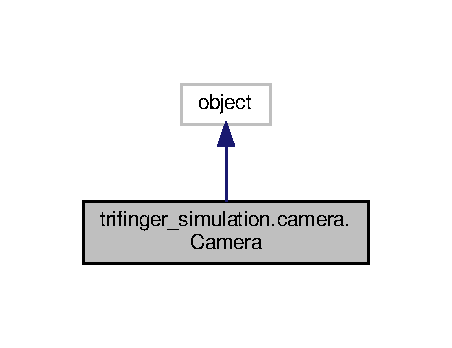
\includegraphics[width=217pt]{classtrifinger__simulation_1_1camera_1_1Camera__inherit__graph}
\end{center}
\end{figure}


Collaboration diagram for trifinger\+\_\+simulation.\+camera.\+Camera\+:
\nopagebreak
\begin{figure}[H]
\begin{center}
\leavevmode
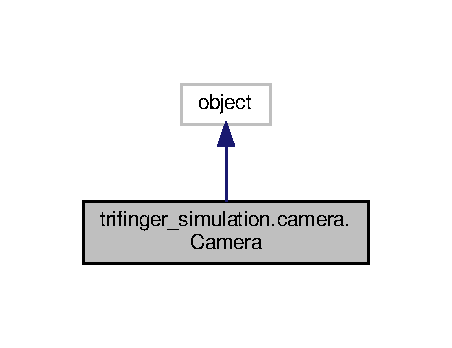
\includegraphics[width=217pt]{classtrifinger__simulation_1_1camera_1_1Camera__coll__graph}
\end{center}
\end{figure}
\subsection*{Public Member Functions}
\begin{DoxyCompactItemize}
\item 
def \hyperlink{classtrifinger__simulation_1_1camera_1_1Camera_a127b955afd7508c05984516b528be056}{\+\_\+\+\_\+init\+\_\+\+\_\+} (self, camera\+\_\+position, camera\+\_\+orientation, image\+\_\+size=(720, 540), pybullet\+\_\+client=pybullet)
\begin{DoxyCompactList}\small\item\em Initialize. \end{DoxyCompactList}\item 
def \hyperlink{classtrifinger__simulation_1_1camera_1_1Camera_a6055089009e1f63df5ced179e5c56254}{get\+\_\+image} (self)
\begin{DoxyCompactList}\small\item\em Get a rendered image from the camera. \end{DoxyCompactList}\end{DoxyCompactItemize}
\subsection*{Private Attributes}
\begin{DoxyCompactItemize}
\item 
\mbox{\Hypertarget{classtrifinger__simulation_1_1camera_1_1Camera_aa5bdad783d26e773b59eb422fb8ea43b}\label{classtrifinger__simulation_1_1camera_1_1Camera_aa5bdad783d26e773b59eb422fb8ea43b}} 
{\bfseries \+\_\+pybullet\+\_\+client}
\item 
\mbox{\Hypertarget{classtrifinger__simulation_1_1camera_1_1Camera_ae6b19b98794b9a6cbe0e7ee3d8e17281}\label{classtrifinger__simulation_1_1camera_1_1Camera_ae6b19b98794b9a6cbe0e7ee3d8e17281}} 
{\bfseries \+\_\+width}
\item 
\mbox{\Hypertarget{classtrifinger__simulation_1_1camera_1_1Camera_abb68a4b72e3d49c124c90e0001735224}\label{classtrifinger__simulation_1_1camera_1_1Camera_abb68a4b72e3d49c124c90e0001735224}} 
{\bfseries \+\_\+height}
\item 
\mbox{\Hypertarget{classtrifinger__simulation_1_1camera_1_1Camera_aafd383344a242bae5b6305ab33bc64ae}\label{classtrifinger__simulation_1_1camera_1_1Camera_aafd383344a242bae5b6305ab33bc64ae}} 
{\bfseries \+\_\+view\+\_\+matrix}
\item 
\mbox{\Hypertarget{classtrifinger__simulation_1_1camera_1_1Camera_a5717913c70a7349ac81d2717325e0fbb}\label{classtrifinger__simulation_1_1camera_1_1Camera_a5717913c70a7349ac81d2717325e0fbb}} 
{\bfseries \+\_\+proj\+\_\+matrix}
\end{DoxyCompactItemize}


\subsection{Detailed Description}
Represents a camera in the simulation environment. 



\subsection{Constructor \& Destructor Documentation}
\mbox{\Hypertarget{classtrifinger__simulation_1_1camera_1_1Camera_a127b955afd7508c05984516b528be056}\label{classtrifinger__simulation_1_1camera_1_1Camera_a127b955afd7508c05984516b528be056}} 
\index{trifinger\+\_\+simulation\+::camera\+::\+Camera@{trifinger\+\_\+simulation\+::camera\+::\+Camera}!\+\_\+\+\_\+init\+\_\+\+\_\+@{\+\_\+\+\_\+init\+\_\+\+\_\+}}
\index{\+\_\+\+\_\+init\+\_\+\+\_\+@{\+\_\+\+\_\+init\+\_\+\+\_\+}!trifinger\+\_\+simulation\+::camera\+::\+Camera@{trifinger\+\_\+simulation\+::camera\+::\+Camera}}
\subsubsection{\texorpdfstring{\+\_\+\+\_\+init\+\_\+\+\_\+()}{\_\_init\_\_()}}
{\footnotesize\ttfamily def trifinger\+\_\+simulation.\+camera.\+Camera.\+\_\+\+\_\+init\+\_\+\+\_\+ (\begin{DoxyParamCaption}\item[{}]{self,  }\item[{}]{camera\+\_\+position,  }\item[{}]{camera\+\_\+orientation,  }\item[{}]{image\+\_\+size = {\ttfamily (720,~540)},  }\item[{}]{pybullet\+\_\+client = {\ttfamily pybullet} }\end{DoxyParamCaption})}



Initialize. 


\begin{DoxyParams}{Parameters}
{\em camera\+\_\+position} & Position (x, y, z) of the camera w.\+r.\+t. the world \\
\hline
{\em frame.} & \\
\hline
{\em camera\+\_\+orientation} & Quaternion (x, y, z, w) representing the orientation of the camera. \\
\hline
{\em image\+\_\+size} & Tuple (width, height) specifying the size of the \\
\hline
{\em image.} & \\
\hline
{\em pybullet\+\_\+client} & Client for accessing the simulation. By default the \char`\"{}pybullet\char`\"{} module is used directly. \\
\hline
\end{DoxyParams}


\subsection{Member Function Documentation}
\mbox{\Hypertarget{classtrifinger__simulation_1_1camera_1_1Camera_a6055089009e1f63df5ced179e5c56254}\label{classtrifinger__simulation_1_1camera_1_1Camera_a6055089009e1f63df5ced179e5c56254}} 
\index{trifinger\+\_\+simulation\+::camera\+::\+Camera@{trifinger\+\_\+simulation\+::camera\+::\+Camera}!get\+\_\+image@{get\+\_\+image}}
\index{get\+\_\+image@{get\+\_\+image}!trifinger\+\_\+simulation\+::camera\+::\+Camera@{trifinger\+\_\+simulation\+::camera\+::\+Camera}}
\subsubsection{\texorpdfstring{get\+\_\+image()}{get\_image()}}
{\footnotesize\ttfamily def trifinger\+\_\+simulation.\+camera.\+Camera.\+get\+\_\+image (\begin{DoxyParamCaption}\item[{}]{self }\end{DoxyParamCaption})}



Get a rendered image from the camera. 

\begin{DoxyReturn}{Returns}
(array, shape=(height, width, 3))\+: Rendered R\+GB image from the simulated camera. 
\end{DoxyReturn}


The documentation for this class was generated from the following file\+:\begin{DoxyCompactItemize}
\item 
python/trifinger\+\_\+simulation/camera.\+py\end{DoxyCompactItemize}

\hypertarget{classtrifinger__simulation_1_1trifinger__platform_1_1CameraObservation}{}\section{trifinger\+\_\+simulation.\+trifinger\+\_\+platform.\+Camera\+Observation Class Reference}
\label{classtrifinger__simulation_1_1trifinger__platform_1_1CameraObservation}\index{trifinger\+\_\+simulation.\+trifinger\+\_\+platform.\+Camera\+Observation@{trifinger\+\_\+simulation.\+trifinger\+\_\+platform.\+Camera\+Observation}}


Pure-\/python copy of trifinger\+\_\+cameras.\+camera.\+Camera\+Observation.  


\subsection*{Public Member Functions}
\begin{DoxyCompactItemize}
\item 
\mbox{\Hypertarget{classtrifinger__simulation_1_1trifinger__platform_1_1CameraObservation_a8c6052304f5d6843c1d6b52f32817175}\label{classtrifinger__simulation_1_1trifinger__platform_1_1CameraObservation_a8c6052304f5d6843c1d6b52f32817175}} 
def {\bfseries \+\_\+\+\_\+init\+\_\+\+\_\+} (self)
\end{DoxyCompactItemize}
\subsection*{Public Attributes}
\begin{DoxyCompactItemize}
\item 
\mbox{\Hypertarget{classtrifinger__simulation_1_1trifinger__platform_1_1CameraObservation_ada255e89c292e56d46ae419f48512eac}\label{classtrifinger__simulation_1_1trifinger__platform_1_1CameraObservation_ada255e89c292e56d46ae419f48512eac}} 
{\bfseries image}
\item 
\mbox{\Hypertarget{classtrifinger__simulation_1_1trifinger__platform_1_1CameraObservation_a4aec6ea871981c158c45fc7e71896dac}\label{classtrifinger__simulation_1_1trifinger__platform_1_1CameraObservation_a4aec6ea871981c158c45fc7e71896dac}} 
{\bfseries timestamp}
\end{DoxyCompactItemize}
\subsection*{Static Private Attributes}
\begin{DoxyCompactItemize}
\item 
\mbox{\Hypertarget{classtrifinger__simulation_1_1trifinger__platform_1_1CameraObservation_a5dd6bdff1185f6b673ae99b796485a66}\label{classtrifinger__simulation_1_1trifinger__platform_1_1CameraObservation_a5dd6bdff1185f6b673ae99b796485a66}} 
list {\bfseries \+\_\+\+\_\+slots\+\_\+\+\_\+} = \mbox{[}\char`\"{}image\char`\"{}, \char`\"{}timestamp\char`\"{}\mbox{]}
\end{DoxyCompactItemize}


\subsection{Detailed Description}
Pure-\/python copy of trifinger\+\_\+cameras.\+camera.\+Camera\+Observation. 



The documentation for this class was generated from the following file\+:\begin{DoxyCompactItemize}
\item 
python/trifinger\+\_\+simulation/trifinger\+\_\+platform.\+py\end{DoxyCompactItemize}

\hypertarget{classtrifinger__simulation_1_1visual__objects_1_1CubeMarker}{}\section{trifinger\+\_\+simulation.\+visual\+\_\+objects.\+Cube\+Marker Class Reference}
\label{classtrifinger__simulation_1_1visual__objects_1_1CubeMarker}\index{trifinger\+\_\+simulation.\+visual\+\_\+objects.\+Cube\+Marker@{trifinger\+\_\+simulation.\+visual\+\_\+objects.\+Cube\+Marker}}


Visualize a cube.  


\subsection*{Public Member Functions}
\begin{DoxyCompactItemize}
\item 
def \hyperlink{classtrifinger__simulation_1_1visual__objects_1_1CubeMarker_a1e9cc5319d4cd0ec27a594c2a4fbb69d}{\+\_\+\+\_\+init\+\_\+\+\_\+} (self, width, position, orientation, color=(0, 1, 0, 0.\+5))
\begin{DoxyCompactList}\small\item\em Create a cube marker for visualization. \end{DoxyCompactList}\item 
def \hyperlink{classtrifinger__simulation_1_1visual__objects_1_1CubeMarker_a76e7dc46d15bc36fa10ec09f18cb2f26}{set\+\_\+state} (self, position, orientation)
\begin{DoxyCompactList}\small\item\em Set pose of the marker. \end{DoxyCompactList}\end{DoxyCompactItemize}
\subsection*{Public Attributes}
\begin{DoxyCompactItemize}
\item 
\mbox{\Hypertarget{classtrifinger__simulation_1_1visual__objects_1_1CubeMarker_ac52687f329f1aef4504ca98369ebce9f}\label{classtrifinger__simulation_1_1visual__objects_1_1CubeMarker_ac52687f329f1aef4504ca98369ebce9f}} 
{\bfseries shape\+\_\+id}
\item 
\mbox{\Hypertarget{classtrifinger__simulation_1_1visual__objects_1_1CubeMarker_a21e3207e9d62ed27ebc2e15b640a4118}\label{classtrifinger__simulation_1_1visual__objects_1_1CubeMarker_a21e3207e9d62ed27ebc2e15b640a4118}} 
{\bfseries body\+\_\+id}
\end{DoxyCompactItemize}


\subsection{Detailed Description}
Visualize a cube. 



\subsection{Constructor \& Destructor Documentation}
\mbox{\Hypertarget{classtrifinger__simulation_1_1visual__objects_1_1CubeMarker_a1e9cc5319d4cd0ec27a594c2a4fbb69d}\label{classtrifinger__simulation_1_1visual__objects_1_1CubeMarker_a1e9cc5319d4cd0ec27a594c2a4fbb69d}} 
\index{trifinger\+\_\+simulation\+::visual\+\_\+objects\+::\+Cube\+Marker@{trifinger\+\_\+simulation\+::visual\+\_\+objects\+::\+Cube\+Marker}!\+\_\+\+\_\+init\+\_\+\+\_\+@{\+\_\+\+\_\+init\+\_\+\+\_\+}}
\index{\+\_\+\+\_\+init\+\_\+\+\_\+@{\+\_\+\+\_\+init\+\_\+\+\_\+}!trifinger\+\_\+simulation\+::visual\+\_\+objects\+::\+Cube\+Marker@{trifinger\+\_\+simulation\+::visual\+\_\+objects\+::\+Cube\+Marker}}
\subsubsection{\texorpdfstring{\+\_\+\+\_\+init\+\_\+\+\_\+()}{\_\_init\_\_()}}
{\footnotesize\ttfamily def trifinger\+\_\+simulation.\+visual\+\_\+objects.\+Cube\+Marker.\+\_\+\+\_\+init\+\_\+\+\_\+ (\begin{DoxyParamCaption}\item[{}]{self,  }\item[{}]{width,  }\item[{}]{position,  }\item[{}]{orientation,  }\item[{}]{color = {\ttfamily (0,~1,~0,~0.5)} }\end{DoxyParamCaption})}



Create a cube marker for visualization. 


\begin{DoxyParams}{Parameters}
{\em width} & Length of one side of the cube. \\
\hline
{\em position} & Position (x, y, z) \\
\hline
{\em orientation} & Orientation as quaternion (x, y, z, w) \\
\hline
{\em color} & Color of the cube as a tuple (r, b, g, q) \\
\hline
\end{DoxyParams}


\subsection{Member Function Documentation}
\mbox{\Hypertarget{classtrifinger__simulation_1_1visual__objects_1_1CubeMarker_a76e7dc46d15bc36fa10ec09f18cb2f26}\label{classtrifinger__simulation_1_1visual__objects_1_1CubeMarker_a76e7dc46d15bc36fa10ec09f18cb2f26}} 
\index{trifinger\+\_\+simulation\+::visual\+\_\+objects\+::\+Cube\+Marker@{trifinger\+\_\+simulation\+::visual\+\_\+objects\+::\+Cube\+Marker}!set\+\_\+state@{set\+\_\+state}}
\index{set\+\_\+state@{set\+\_\+state}!trifinger\+\_\+simulation\+::visual\+\_\+objects\+::\+Cube\+Marker@{trifinger\+\_\+simulation\+::visual\+\_\+objects\+::\+Cube\+Marker}}
\subsubsection{\texorpdfstring{set\+\_\+state()}{set\_state()}}
{\footnotesize\ttfamily def trifinger\+\_\+simulation.\+visual\+\_\+objects.\+Cube\+Marker.\+set\+\_\+state (\begin{DoxyParamCaption}\item[{}]{self,  }\item[{}]{position,  }\item[{}]{orientation }\end{DoxyParamCaption})}



Set pose of the marker. 


\begin{DoxyParams}{Parameters}
{\em position} & Position (x, y, z) \\
\hline
{\em orientation} & Orientation as quaternion (x, y, z, w) \\
\hline
\end{DoxyParams}


The documentation for this class was generated from the following file\+:\begin{DoxyCompactItemize}
\item 
python/trifinger\+\_\+simulation/visual\+\_\+objects.\+py\end{DoxyCompactItemize}

\hypertarget{classtrifinger__simulation_1_1gym__wrapper_1_1data__logger_1_1DataLogger}{}\section{trifinger\+\_\+simulation.\+gym\+\_\+wrapper.\+data\+\_\+logger.\+Data\+Logger Class Reference}
\label{classtrifinger__simulation_1_1gym__wrapper_1_1data__logger_1_1DataLogger}\index{trifinger\+\_\+simulation.\+gym\+\_\+wrapper.\+data\+\_\+logger.\+Data\+Logger@{trifinger\+\_\+simulation.\+gym\+\_\+wrapper.\+data\+\_\+logger.\+Data\+Logger}}


Dumps the env episodic data to a pickle file.  


\subsection*{Public Member Functions}
\begin{DoxyCompactItemize}
\item 
\mbox{\Hypertarget{classtrifinger__simulation_1_1gym__wrapper_1_1data__logger_1_1DataLogger_a8c8b07484dfbf15cb1e3c2e89fcf51c0}\label{classtrifinger__simulation_1_1gym__wrapper_1_1data__logger_1_1DataLogger_a8c8b07484dfbf15cb1e3c2e89fcf51c0}} 
def {\bfseries \+\_\+\+\_\+init\+\_\+\+\_\+} (self)
\item 
\mbox{\Hypertarget{classtrifinger__simulation_1_1gym__wrapper_1_1data__logger_1_1DataLogger_a818fe6118c20bd1498bd7e1f2700105b}\label{classtrifinger__simulation_1_1gym__wrapper_1_1data__logger_1_1DataLogger_a818fe6118c20bd1498bd7e1f2700105b}} 
def {\bfseries new\+\_\+episode} (self, joint\+\_\+goal, tip\+\_\+goal)
\item 
\mbox{\Hypertarget{classtrifinger__simulation_1_1gym__wrapper_1_1data__logger_1_1DataLogger_a2b128c4f1dc3f8ffc4b86357707dbf09}\label{classtrifinger__simulation_1_1gym__wrapper_1_1data__logger_1_1DataLogger_a2b128c4f1dc3f8ffc4b86357707dbf09}} 
def {\bfseries append} (self, joint\+\_\+pos, tip\+\_\+pos, timestamp)
\item 
\mbox{\Hypertarget{classtrifinger__simulation_1_1gym__wrapper_1_1data__logger_1_1DataLogger_acc5c4317ab74121615c8c2c86973b740}\label{classtrifinger__simulation_1_1gym__wrapper_1_1data__logger_1_1DataLogger_acc5c4317ab74121615c8c2c86973b740}} 
def {\bfseries store} (self, filename)
\end{DoxyCompactItemize}
\subsection*{Public Attributes}
\begin{DoxyCompactItemize}
\item 
\mbox{\Hypertarget{classtrifinger__simulation_1_1gym__wrapper_1_1data__logger_1_1DataLogger_afaf8d0d5636dfa406e240991ad665acf}\label{classtrifinger__simulation_1_1gym__wrapper_1_1data__logger_1_1DataLogger_afaf8d0d5636dfa406e240991ad665acf}} 
{\bfseries episodes}
\end{DoxyCompactItemize}
\subsection*{Private Attributes}
\begin{DoxyCompactItemize}
\item 
\mbox{\Hypertarget{classtrifinger__simulation_1_1gym__wrapper_1_1data__logger_1_1DataLogger_a855bce5dc38c90b0c0cfc1a6c034c511}\label{classtrifinger__simulation_1_1gym__wrapper_1_1data__logger_1_1DataLogger_a855bce5dc38c90b0c0cfc1a6c034c511}} 
{\bfseries \+\_\+curr}
\end{DoxyCompactItemize}


\subsection{Detailed Description}
Dumps the env episodic data to a pickle file. 

The documentation for this class was generated from the following file\+:\begin{DoxyCompactItemize}
\item 
python/trifinger\+\_\+simulation/gym\+\_\+wrapper/data\+\_\+logger.\+py\end{DoxyCompactItemize}

\hypertarget{classtrifinger__simulation_1_1gym__wrapper_1_1data__logger_1_1EpisodeData}{}\section{trifinger\+\_\+simulation.\+gym\+\_\+wrapper.\+data\+\_\+logger.\+Episode\+Data Class Reference}
\label{classtrifinger__simulation_1_1gym__wrapper_1_1data__logger_1_1EpisodeData}\index{trifinger\+\_\+simulation.\+gym\+\_\+wrapper.\+data\+\_\+logger.\+Episode\+Data@{trifinger\+\_\+simulation.\+gym\+\_\+wrapper.\+data\+\_\+logger.\+Episode\+Data}}
\subsection*{Public Member Functions}
\begin{DoxyCompactItemize}
\item 
\mbox{\Hypertarget{classtrifinger__simulation_1_1gym__wrapper_1_1data__logger_1_1EpisodeData_a995b85cb8a75c0f9b513cb65ba0f6d4f}\label{classtrifinger__simulation_1_1gym__wrapper_1_1data__logger_1_1EpisodeData_a995b85cb8a75c0f9b513cb65ba0f6d4f}} 
def {\bfseries \+\_\+\+\_\+init\+\_\+\+\_\+} (self, joint\+\_\+goal, tip\+\_\+goal)
\item 
\mbox{\Hypertarget{classtrifinger__simulation_1_1gym__wrapper_1_1data__logger_1_1EpisodeData_ae7b701ac5f0cc636f4e35494088457f8}\label{classtrifinger__simulation_1_1gym__wrapper_1_1data__logger_1_1EpisodeData_ae7b701ac5f0cc636f4e35494088457f8}} 
def {\bfseries append} (self, joint\+\_\+pos, tip\+\_\+pos, timestamp)
\end{DoxyCompactItemize}
\subsection*{Public Attributes}
\begin{DoxyCompactItemize}
\item 
\mbox{\Hypertarget{classtrifinger__simulation_1_1gym__wrapper_1_1data__logger_1_1EpisodeData_a202f68a21b4e57bf292a8fbb67fcb4a6}\label{classtrifinger__simulation_1_1gym__wrapper_1_1data__logger_1_1EpisodeData_a202f68a21b4e57bf292a8fbb67fcb4a6}} 
{\bfseries joint\+\_\+goal}
\item 
\mbox{\Hypertarget{classtrifinger__simulation_1_1gym__wrapper_1_1data__logger_1_1EpisodeData_a4b0d1e86244d42540cf1564ffbaf0086}\label{classtrifinger__simulation_1_1gym__wrapper_1_1data__logger_1_1EpisodeData_a4b0d1e86244d42540cf1564ffbaf0086}} 
{\bfseries tip\+\_\+goal}
\item 
\mbox{\Hypertarget{classtrifinger__simulation_1_1gym__wrapper_1_1data__logger_1_1EpisodeData_a221bc67e1473d1b5becff014b2914ffe}\label{classtrifinger__simulation_1_1gym__wrapper_1_1data__logger_1_1EpisodeData_a221bc67e1473d1b5becff014b2914ffe}} 
{\bfseries joint\+\_\+positions}
\item 
\mbox{\Hypertarget{classtrifinger__simulation_1_1gym__wrapper_1_1data__logger_1_1EpisodeData_a3d6a04f83f862d48be0e9b2500d5000c}\label{classtrifinger__simulation_1_1gym__wrapper_1_1data__logger_1_1EpisodeData_a3d6a04f83f862d48be0e9b2500d5000c}} 
{\bfseries tip\+\_\+positions}
\item 
\mbox{\Hypertarget{classtrifinger__simulation_1_1gym__wrapper_1_1data__logger_1_1EpisodeData_a7cebf91d27c7060d8eccb2c975f368e7}\label{classtrifinger__simulation_1_1gym__wrapper_1_1data__logger_1_1EpisodeData_a7cebf91d27c7060d8eccb2c975f368e7}} 
{\bfseries timestamps}
\end{DoxyCompactItemize}


The documentation for this class was generated from the following file\+:\begin{DoxyCompactItemize}
\item 
python/trifinger\+\_\+simulation/gym\+\_\+wrapper/data\+\_\+logger.\+py\end{DoxyCompactItemize}

\hypertarget{classexample__pushing__training__env_1_1ExamplePushingTrainingEnv}{}\section{example\+\_\+pushing\+\_\+training\+\_\+env.\+Example\+Pushing\+Training\+Env Class Reference}
\label{classexample__pushing__training__env_1_1ExamplePushingTrainingEnv}\index{example\+\_\+pushing\+\_\+training\+\_\+env.\+Example\+Pushing\+Training\+Env@{example\+\_\+pushing\+\_\+training\+\_\+env.\+Example\+Pushing\+Training\+Env}}


Gym environment for moving cubes with simulated Tri\+Finger\+Pro.  




Inheritance diagram for example\+\_\+pushing\+\_\+training\+\_\+env.\+Example\+Pushing\+Training\+Env\+:
\nopagebreak
\begin{figure}[H]
\begin{center}
\leavevmode
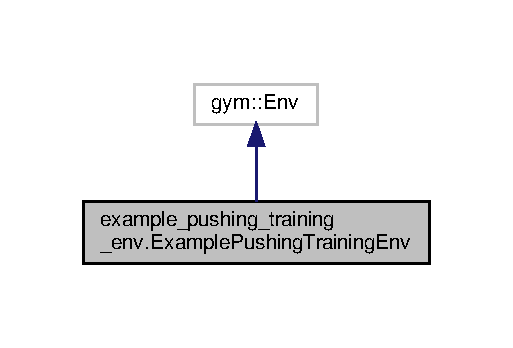
\includegraphics[width=246pt]{classexample__pushing__training__env_1_1ExamplePushingTrainingEnv__inherit__graph}
\end{center}
\end{figure}


Collaboration diagram for example\+\_\+pushing\+\_\+training\+\_\+env.\+Example\+Pushing\+Training\+Env\+:
\nopagebreak
\begin{figure}[H]
\begin{center}
\leavevmode
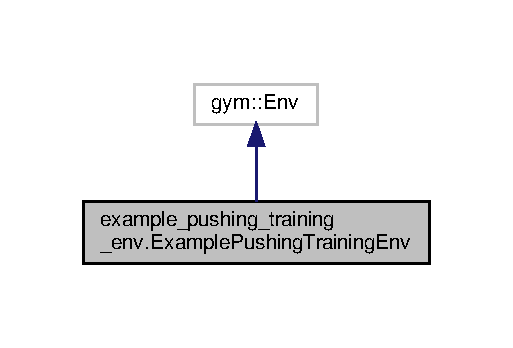
\includegraphics[width=246pt]{classexample__pushing__training__env_1_1ExamplePushingTrainingEnv__coll__graph}
\end{center}
\end{figure}
\subsection*{Public Member Functions}
\begin{DoxyCompactItemize}
\item 
def \hyperlink{classexample__pushing__training__env_1_1ExamplePushingTrainingEnv_a1b542291e45e2b2c267b8a240193e0b4}{\+\_\+\+\_\+init\+\_\+\+\_\+} (self, initializer=None, action\+\_\+type=cube\+\_\+env.\+Action\+Type.\+P\+O\+S\+I\+T\+I\+ON, frameskip=1, visualization=False)
\begin{DoxyCompactList}\small\item\em Initialize. \end{DoxyCompactList}\item 
\mbox{\Hypertarget{classexample__pushing__training__env_1_1ExamplePushingTrainingEnv_a92e5f26d7d80d93b686c97dce911874d}\label{classexample__pushing__training__env_1_1ExamplePushingTrainingEnv_a92e5f26d7d80d93b686c97dce911874d}} 
def {\bfseries step} (self, action)
\item 
\mbox{\Hypertarget{classexample__pushing__training__env_1_1ExamplePushingTrainingEnv_a592d95e4040bb362f438849df5fa6fc8}\label{classexample__pushing__training__env_1_1ExamplePushingTrainingEnv_a592d95e4040bb362f438849df5fa6fc8}} 
def {\bfseries reset} (self)
\item 
\mbox{\Hypertarget{classexample__pushing__training__env_1_1ExamplePushingTrainingEnv_a6873cea9e63b86cc3565c1cd914747be}\label{classexample__pushing__training__env_1_1ExamplePushingTrainingEnv_a6873cea9e63b86cc3565c1cd914747be}} 
def {\bfseries seed} (self, seed=None)
\end{DoxyCompactItemize}
\subsection*{Public Attributes}
\begin{DoxyCompactItemize}
\item 
\mbox{\Hypertarget{classexample__pushing__training__env_1_1ExamplePushingTrainingEnv_a76d3f87af01e8738a8edecde7c2ab600}\label{classexample__pushing__training__env_1_1ExamplePushingTrainingEnv_a76d3f87af01e8738a8edecde7c2ab600}} 
{\bfseries initializer}
\item 
\mbox{\Hypertarget{classexample__pushing__training__env_1_1ExamplePushingTrainingEnv_a06f4c145bdb601d5075a42be9b528c06}\label{classexample__pushing__training__env_1_1ExamplePushingTrainingEnv_a06f4c145bdb601d5075a42be9b528c06}} 
{\bfseries action\+\_\+type}
\item 
\mbox{\Hypertarget{classexample__pushing__training__env_1_1ExamplePushingTrainingEnv_a2aafa7d24a9ecdebd69fc68f774513c2}\label{classexample__pushing__training__env_1_1ExamplePushingTrainingEnv_a2aafa7d24a9ecdebd69fc68f774513c2}} 
{\bfseries visualization}
\item 
\mbox{\Hypertarget{classexample__pushing__training__env_1_1ExamplePushingTrainingEnv_adff797f22690bfc65c0076d7f5b14dd3}\label{classexample__pushing__training__env_1_1ExamplePushingTrainingEnv_adff797f22690bfc65c0076d7f5b14dd3}} 
{\bfseries frameskip}
\item 
\mbox{\Hypertarget{classexample__pushing__training__env_1_1ExamplePushingTrainingEnv_a2f517c0b2e277cefc385c8a540f117a4}\label{classexample__pushing__training__env_1_1ExamplePushingTrainingEnv_a2f517c0b2e277cefc385c8a540f117a4}} 
{\bfseries platform}
\item 
\mbox{\Hypertarget{classexample__pushing__training__env_1_1ExamplePushingTrainingEnv_ad8a7374f98fb7c5c1cbe91fbd81a5c1c}\label{classexample__pushing__training__env_1_1ExamplePushingTrainingEnv_ad8a7374f98fb7c5c1cbe91fbd81a5c1c}} 
{\bfseries action\+\_\+space}
\item 
\mbox{\Hypertarget{classexample__pushing__training__env_1_1ExamplePushingTrainingEnv_a85e87056ef0026f13678e604a624a870}\label{classexample__pushing__training__env_1_1ExamplePushingTrainingEnv_a85e87056ef0026f13678e604a624a870}} 
{\bfseries observation\+\_\+names}
\item 
\mbox{\Hypertarget{classexample__pushing__training__env_1_1ExamplePushingTrainingEnv_adff2539cd296c946ee108f0c82623448}\label{classexample__pushing__training__env_1_1ExamplePushingTrainingEnv_adff2539cd296c946ee108f0c82623448}} 
{\bfseries observation\+\_\+space}
\item 
\mbox{\Hypertarget{classexample__pushing__training__env_1_1ExamplePushingTrainingEnv_a28d37c465544f27018ebf1d9a215604e}\label{classexample__pushing__training__env_1_1ExamplePushingTrainingEnv_a28d37c465544f27018ebf1d9a215604e}} 
{\bfseries step\+\_\+count}
\item 
\mbox{\Hypertarget{classexample__pushing__training__env_1_1ExamplePushingTrainingEnv_afb6af65aa630dfbd82a377f7116dc218}\label{classexample__pushing__training__env_1_1ExamplePushingTrainingEnv_afb6af65aa630dfbd82a377f7116dc218}} 
{\bfseries goal}
\item 
\mbox{\Hypertarget{classexample__pushing__training__env_1_1ExamplePushingTrainingEnv_a364d2a71dace6a8d7aa7853711284279}\label{classexample__pushing__training__env_1_1ExamplePushingTrainingEnv_a364d2a71dace6a8d7aa7853711284279}} 
{\bfseries goal\+\_\+marker}
\item 
\mbox{\Hypertarget{classexample__pushing__training__env_1_1ExamplePushingTrainingEnv_a3fe1c7b6d4b868f82e6d526642b10c91}\label{classexample__pushing__training__env_1_1ExamplePushingTrainingEnv_a3fe1c7b6d4b868f82e6d526642b10c91}} 
{\bfseries info}
\end{DoxyCompactItemize}
\subsection*{Private Member Functions}
\begin{DoxyCompactItemize}
\item 
\mbox{\Hypertarget{classexample__pushing__training__env_1_1ExamplePushingTrainingEnv_afbb847a8de2b991324ec7c6e55e1ba5a}\label{classexample__pushing__training__env_1_1ExamplePushingTrainingEnv_afbb847a8de2b991324ec7c6e55e1ba5a}} 
def {\bfseries \+\_\+create\+\_\+observation} (self, t)
\item 
\mbox{\Hypertarget{classexample__pushing__training__env_1_1ExamplePushingTrainingEnv_a1e3940e8da32823a3e18e58bb0925285}\label{classexample__pushing__training__env_1_1ExamplePushingTrainingEnv_a1e3940e8da32823a3e18e58bb0925285}} 
def {\bfseries \+\_\+gym\+\_\+action\+\_\+to\+\_\+robot\+\_\+action} (self, gym\+\_\+action)
\end{DoxyCompactItemize}
\subsection*{Static Private Member Functions}
\begin{DoxyCompactItemize}
\item 
\mbox{\Hypertarget{classexample__pushing__training__env_1_1ExamplePushingTrainingEnv_ae9b0a300dcce6c7ebc7a5b85d11f3651}\label{classexample__pushing__training__env_1_1ExamplePushingTrainingEnv_ae9b0a300dcce6c7ebc7a5b85d11f3651}} 
def {\bfseries \+\_\+compute\+\_\+reward} (previous\+\_\+observation, observation)
\end{DoxyCompactItemize}


\subsection{Detailed Description}
Gym environment for moving cubes with simulated Tri\+Finger\+Pro. 



\subsection{Constructor \& Destructor Documentation}
\mbox{\Hypertarget{classexample__pushing__training__env_1_1ExamplePushingTrainingEnv_a1b542291e45e2b2c267b8a240193e0b4}\label{classexample__pushing__training__env_1_1ExamplePushingTrainingEnv_a1b542291e45e2b2c267b8a240193e0b4}} 
\index{example\+\_\+pushing\+\_\+training\+\_\+env\+::\+Example\+Pushing\+Training\+Env@{example\+\_\+pushing\+\_\+training\+\_\+env\+::\+Example\+Pushing\+Training\+Env}!\+\_\+\+\_\+init\+\_\+\+\_\+@{\+\_\+\+\_\+init\+\_\+\+\_\+}}
\index{\+\_\+\+\_\+init\+\_\+\+\_\+@{\+\_\+\+\_\+init\+\_\+\+\_\+}!example\+\_\+pushing\+\_\+training\+\_\+env\+::\+Example\+Pushing\+Training\+Env@{example\+\_\+pushing\+\_\+training\+\_\+env\+::\+Example\+Pushing\+Training\+Env}}
\subsubsection{\texorpdfstring{\+\_\+\+\_\+init\+\_\+\+\_\+()}{\_\_init\_\_()}}
{\footnotesize\ttfamily def example\+\_\+pushing\+\_\+training\+\_\+env.\+Example\+Pushing\+Training\+Env.\+\_\+\+\_\+init\+\_\+\+\_\+ (\begin{DoxyParamCaption}\item[{}]{self,  }\item[{}]{initializer = {\ttfamily None},  }\item[{}]{action\+\_\+type = {\ttfamily cube\+\_\+env.ActionType.POSITION},  }\item[{}]{frameskip = {\ttfamily 1},  }\item[{}]{visualization = {\ttfamily False} }\end{DoxyParamCaption})}



Initialize. 


\begin{DoxyParams}{Parameters}
{\em initializer} & Initializer class for providing initial cube pose and goal pose. If no initializer is provided, we will initialize in a way which is be helpful for learning. \\
\hline
{\em action\+\_\+type} & Specify which type of actions to use. See \+:class\+:{\ttfamily Action\+Type} for details. \\
\hline
{\em frameskip} & Number of actual control steps to be performed in one call of step(). \\
\hline
{\em visualization} & If true, the py\+Bullet G\+UI is run for \\
\hline
{\em visualization.} & \\
\hline
\end{DoxyParams}


The documentation for this class was generated from the following file\+:\begin{DoxyCompactItemize}
\item 
example/example\+\_\+pushing\+\_\+training\+\_\+env.\+py\end{DoxyCompactItemize}

\hypertarget{classtrifinger__simulation_1_1gym__wrapper_1_1finger__spaces_1_1FingerSpaces}{}\section{trifinger\+\_\+simulation.\+gym\+\_\+wrapper.\+finger\+\_\+spaces.\+Finger\+Spaces Class Reference}
\label{classtrifinger__simulation_1_1gym__wrapper_1_1finger__spaces_1_1FingerSpaces}\index{trifinger\+\_\+simulation.\+gym\+\_\+wrapper.\+finger\+\_\+spaces.\+Finger\+Spaces@{trifinger\+\_\+simulation.\+gym\+\_\+wrapper.\+finger\+\_\+spaces.\+Finger\+Spaces}}
\subsection*{Public Member Functions}
\begin{DoxyCompactItemize}
\item 
\mbox{\Hypertarget{classtrifinger__simulation_1_1gym__wrapper_1_1finger__spaces_1_1FingerSpaces_a7193543098a4655e7d5a63c133d0d399}\label{classtrifinger__simulation_1_1gym__wrapper_1_1finger__spaces_1_1FingerSpaces_a7193543098a4655e7d5a63c133d0d399}} 
def {\bfseries \+\_\+\+\_\+init\+\_\+\+\_\+} (self, num\+\_\+fingers, observations\+\_\+keys, observations\+\_\+sizes, separate\+\_\+goals)
\item 
\mbox{\Hypertarget{classtrifinger__simulation_1_1gym__wrapper_1_1finger__spaces_1_1FingerSpaces_a71bba5fe8e1228d14d5394745d173e09}\label{classtrifinger__simulation_1_1gym__wrapper_1_1finger__spaces_1_1FingerSpaces_a71bba5fe8e1228d14d5394745d173e09}} 
def {\bfseries get\+\_\+unscaled\+\_\+observation\+\_\+space} (self)
\item 
\mbox{\Hypertarget{classtrifinger__simulation_1_1gym__wrapper_1_1finger__spaces_1_1FingerSpaces_a839d244f6a939aff8c2f1fb2ed2a33df}\label{classtrifinger__simulation_1_1gym__wrapper_1_1finger__spaces_1_1FingerSpaces_a839d244f6a939aff8c2f1fb2ed2a33df}} 
def \hyperlink{classtrifinger__simulation_1_1gym__wrapper_1_1finger__spaces_1_1FingerSpaces_a839d244f6a939aff8c2f1fb2ed2a33df}{get\+\_\+unscaled\+\_\+action\+\_\+space} (self)
\begin{DoxyCompactList}\small\item\em Returns the unscaled action space according to the action bounds. \end{DoxyCompactList}\item 
\mbox{\Hypertarget{classtrifinger__simulation_1_1gym__wrapper_1_1finger__spaces_1_1FingerSpaces_a3a2f00342767679322d45091cb4eecdf}\label{classtrifinger__simulation_1_1gym__wrapper_1_1finger__spaces_1_1FingerSpaces_a3a2f00342767679322d45091cb4eecdf}} 
def {\bfseries get\+\_\+scaled\+\_\+observation\+\_\+space} (self)
\item 
\mbox{\Hypertarget{classtrifinger__simulation_1_1gym__wrapper_1_1finger__spaces_1_1FingerSpaces_ab0379b8f1ffc1951be8f6ac870b6f31e}\label{classtrifinger__simulation_1_1gym__wrapper_1_1finger__spaces_1_1FingerSpaces_ab0379b8f1ffc1951be8f6ac870b6f31e}} 
def {\bfseries get\+\_\+scaled\+\_\+action\+\_\+space} (self)
\end{DoxyCompactItemize}
\subsection*{Public Attributes}
\begin{DoxyCompactItemize}
\item 
\mbox{\Hypertarget{classtrifinger__simulation_1_1gym__wrapper_1_1finger__spaces_1_1FingerSpaces_aef6a5facf4a5770bb52d7e118f27092b}\label{classtrifinger__simulation_1_1gym__wrapper_1_1finger__spaces_1_1FingerSpaces_aef6a5facf4a5770bb52d7e118f27092b}} 
{\bfseries num\+\_\+fingers}
\item 
\mbox{\Hypertarget{classtrifinger__simulation_1_1gym__wrapper_1_1finger__spaces_1_1FingerSpaces_ae48dce07f3223ad09ed3752f8a4ca267}\label{classtrifinger__simulation_1_1gym__wrapper_1_1finger__spaces_1_1FingerSpaces_ae48dce07f3223ad09ed3752f8a4ca267}} 
{\bfseries lower\+\_\+bounds}
\item 
\mbox{\Hypertarget{classtrifinger__simulation_1_1gym__wrapper_1_1finger__spaces_1_1FingerSpaces_af942cd00b37c2e51bccfb724b4bcced2}\label{classtrifinger__simulation_1_1gym__wrapper_1_1finger__spaces_1_1FingerSpaces_af942cd00b37c2e51bccfb724b4bcced2}} 
{\bfseries upper\+\_\+bounds}
\item 
\mbox{\Hypertarget{classtrifinger__simulation_1_1gym__wrapper_1_1finger__spaces_1_1FingerSpaces_a9b82d691aebb956d9920063ff7f9169b}\label{classtrifinger__simulation_1_1gym__wrapper_1_1finger__spaces_1_1FingerSpaces_a9b82d691aebb956d9920063ff7f9169b}} 
{\bfseries observations\+\_\+keys}
\item 
\mbox{\Hypertarget{classtrifinger__simulation_1_1gym__wrapper_1_1finger__spaces_1_1FingerSpaces_a6cff11eb6d063691df77044a78c348b3}\label{classtrifinger__simulation_1_1gym__wrapper_1_1finger__spaces_1_1FingerSpaces_a6cff11eb6d063691df77044a78c348b3}} 
{\bfseries observations\+\_\+sizes}
\item 
\mbox{\Hypertarget{classtrifinger__simulation_1_1gym__wrapper_1_1finger__spaces_1_1FingerSpaces_a4ba608cf0a602268b70c96ef7085401a}\label{classtrifinger__simulation_1_1gym__wrapper_1_1finger__spaces_1_1FingerSpaces_a4ba608cf0a602268b70c96ef7085401a}} 
{\bfseries key\+\_\+to\+\_\+index}
\item 
\mbox{\Hypertarget{classtrifinger__simulation_1_1gym__wrapper_1_1finger__spaces_1_1FingerSpaces_a3484888d7e750fef3d594e26545d32b5}\label{classtrifinger__simulation_1_1gym__wrapper_1_1finger__spaces_1_1FingerSpaces_a3484888d7e750fef3d594e26545d32b5}} 
{\bfseries separate\+\_\+goals}
\item 
\mbox{\Hypertarget{classtrifinger__simulation_1_1gym__wrapper_1_1finger__spaces_1_1FingerSpaces_a61429f2ddc51fd47df9a296a5e32a707}\label{classtrifinger__simulation_1_1gym__wrapper_1_1finger__spaces_1_1FingerSpaces_a61429f2ddc51fd47df9a296a5e32a707}} 
{\bfseries action\+\_\+bounds}
\end{DoxyCompactItemize}


The documentation for this class was generated from the following file\+:\begin{DoxyCompactItemize}
\item 
python/trifinger\+\_\+simulation/gym\+\_\+wrapper/finger\+\_\+spaces.\+py\end{DoxyCompactItemize}

\hypertarget{classtrifinger__simulation_1_1finger__types__data_1_1FingerTypesDataFormat}{}\section{trifinger\+\_\+simulation.\+finger\+\_\+types\+\_\+data.\+Finger\+Types\+Data\+Format Class Reference}
\label{classtrifinger__simulation_1_1finger__types__data_1_1FingerTypesDataFormat}\index{trifinger\+\_\+simulation.\+finger\+\_\+types\+\_\+data.\+Finger\+Types\+Data\+Format@{trifinger\+\_\+simulation.\+finger\+\_\+types\+\_\+data.\+Finger\+Types\+Data\+Format}}


Describes the format for the finger type data, comprising of the corresponding urdf, and the number of fingers.  




Inheritance diagram for trifinger\+\_\+simulation.\+finger\+\_\+types\+\_\+data.\+Finger\+Types\+Data\+Format\+:
\nopagebreak
\begin{figure}[H]
\begin{center}
\leavevmode
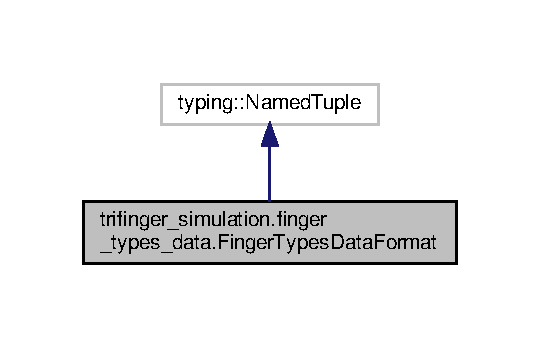
\includegraphics[width=259pt]{classtrifinger__simulation_1_1finger__types__data_1_1FingerTypesDataFormat__inherit__graph}
\end{center}
\end{figure}


Collaboration diagram for trifinger\+\_\+simulation.\+finger\+\_\+types\+\_\+data.\+Finger\+Types\+Data\+Format\+:
\nopagebreak
\begin{figure}[H]
\begin{center}
\leavevmode
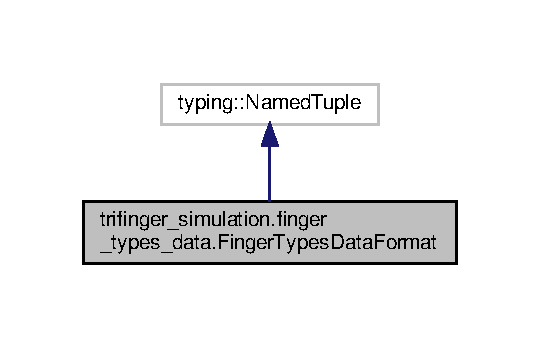
\includegraphics[width=259pt]{classtrifinger__simulation_1_1finger__types__data_1_1FingerTypesDataFormat__coll__graph}
\end{center}
\end{figure}


\subsection{Detailed Description}
Describes the format for the finger type data, comprising of the corresponding urdf, and the number of fingers. 

The documentation for this class was generated from the following file\+:\begin{DoxyCompactItemize}
\item 
python/trifinger\+\_\+simulation/finger\+\_\+types\+\_\+data.\+py\end{DoxyCompactItemize}

\hypertarget{classexample__pushing__training__env_1_1FlatObservationWrapper}{}\section{example\+\_\+pushing\+\_\+training\+\_\+env.\+Flat\+Observation\+Wrapper Class Reference}
\label{classexample__pushing__training__env_1_1FlatObservationWrapper}\index{example\+\_\+pushing\+\_\+training\+\_\+env.\+Flat\+Observation\+Wrapper@{example\+\_\+pushing\+\_\+training\+\_\+env.\+Flat\+Observation\+Wrapper}}


Inheritance diagram for example\+\_\+pushing\+\_\+training\+\_\+env.\+Flat\+Observation\+Wrapper\+:
\nopagebreak
\begin{figure}[H]
\begin{center}
\leavevmode
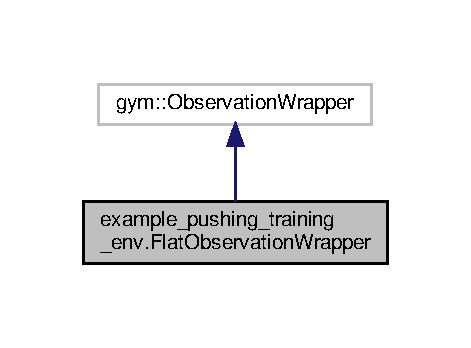
\includegraphics[width=226pt]{classexample__pushing__training__env_1_1FlatObservationWrapper__inherit__graph}
\end{center}
\end{figure}


Collaboration diagram for example\+\_\+pushing\+\_\+training\+\_\+env.\+Flat\+Observation\+Wrapper\+:
\nopagebreak
\begin{figure}[H]
\begin{center}
\leavevmode
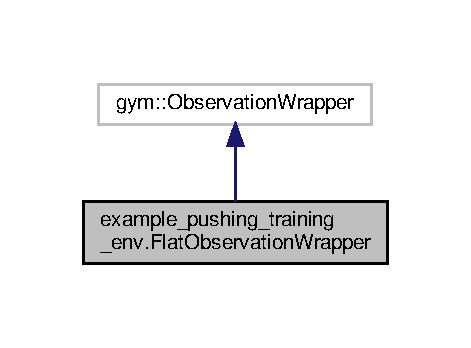
\includegraphics[width=226pt]{classexample__pushing__training__env_1_1FlatObservationWrapper__coll__graph}
\end{center}
\end{figure}
\subsection*{Public Member Functions}
\begin{DoxyCompactItemize}
\item 
\mbox{\Hypertarget{classexample__pushing__training__env_1_1FlatObservationWrapper_a6de061353278330c014b51c069c3f49d}\label{classexample__pushing__training__env_1_1FlatObservationWrapper_a6de061353278330c014b51c069c3f49d}} 
def {\bfseries \+\_\+\+\_\+init\+\_\+\+\_\+} (self, env)
\item 
\mbox{\Hypertarget{classexample__pushing__training__env_1_1FlatObservationWrapper_a7d3d597817e12bfa7eb42c335e6fc65c}\label{classexample__pushing__training__env_1_1FlatObservationWrapper_a7d3d597817e12bfa7eb42c335e6fc65c}} 
def {\bfseries observation} (self, obs)
\end{DoxyCompactItemize}
\subsection*{Public Attributes}
\begin{DoxyCompactItemize}
\item 
\mbox{\Hypertarget{classexample__pushing__training__env_1_1FlatObservationWrapper_a38c76cd02dbeffe8cbb4808e6f77249a}\label{classexample__pushing__training__env_1_1FlatObservationWrapper_a38c76cd02dbeffe8cbb4808e6f77249a}} 
{\bfseries observation\+\_\+space}
\end{DoxyCompactItemize}


The documentation for this class was generated from the following file\+:\begin{DoxyCompactItemize}
\item 
example/example\+\_\+pushing\+\_\+training\+\_\+env.\+py\end{DoxyCompactItemize}

\hypertarget{classtrifinger__simulation_1_1tasks_1_1move__cube_1_1InvalidGoalError}{}\section{trifinger\+\_\+simulation.\+tasks.\+move\+\_\+cube.\+Invalid\+Goal\+Error Class Reference}
\label{classtrifinger__simulation_1_1tasks_1_1move__cube_1_1InvalidGoalError}\index{trifinger\+\_\+simulation.\+tasks.\+move\+\_\+cube.\+Invalid\+Goal\+Error@{trifinger\+\_\+simulation.\+tasks.\+move\+\_\+cube.\+Invalid\+Goal\+Error}}


Exception used to indicate that the given goal is invalid.  




Inheritance diagram for trifinger\+\_\+simulation.\+tasks.\+move\+\_\+cube.\+Invalid\+Goal\+Error\+:
\nopagebreak
\begin{figure}[H]
\begin{center}
\leavevmode
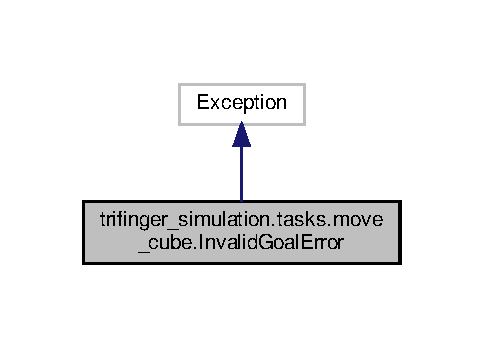
\includegraphics[width=232pt]{classtrifinger__simulation_1_1tasks_1_1move__cube_1_1InvalidGoalError__inherit__graph}
\end{center}
\end{figure}


Collaboration diagram for trifinger\+\_\+simulation.\+tasks.\+move\+\_\+cube.\+Invalid\+Goal\+Error\+:
\nopagebreak
\begin{figure}[H]
\begin{center}
\leavevmode
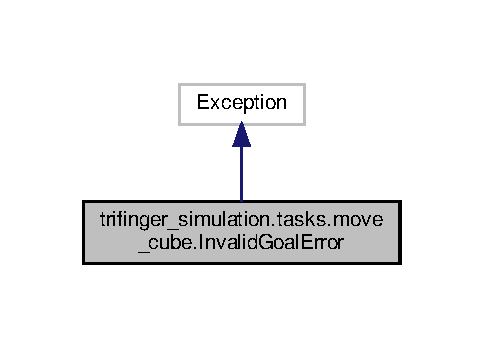
\includegraphics[width=232pt]{classtrifinger__simulation_1_1tasks_1_1move__cube_1_1InvalidGoalError__coll__graph}
\end{center}
\end{figure}
\subsection*{Public Member Functions}
\begin{DoxyCompactItemize}
\item 
\mbox{\Hypertarget{classtrifinger__simulation_1_1tasks_1_1move__cube_1_1InvalidGoalError_a615089ce5f1379b4c176cb13848fa4cf}\label{classtrifinger__simulation_1_1tasks_1_1move__cube_1_1InvalidGoalError_a615089ce5f1379b4c176cb13848fa4cf}} 
def {\bfseries \+\_\+\+\_\+init\+\_\+\+\_\+} (self, message, position, orientation)
\end{DoxyCompactItemize}
\subsection*{Public Attributes}
\begin{DoxyCompactItemize}
\item 
\mbox{\Hypertarget{classtrifinger__simulation_1_1tasks_1_1move__cube_1_1InvalidGoalError_a1f31c828b3dc9464138709c5a9e8a7d4}\label{classtrifinger__simulation_1_1tasks_1_1move__cube_1_1InvalidGoalError_a1f31c828b3dc9464138709c5a9e8a7d4}} 
{\bfseries position}
\item 
\mbox{\Hypertarget{classtrifinger__simulation_1_1tasks_1_1move__cube_1_1InvalidGoalError_ab4318be287d0fea40510bef529ef540a}\label{classtrifinger__simulation_1_1tasks_1_1move__cube_1_1InvalidGoalError_ab4318be287d0fea40510bef529ef540a}} 
{\bfseries orientation}
\end{DoxyCompactItemize}


\subsection{Detailed Description}
Exception used to indicate that the given goal is invalid. 



The documentation for this class was generated from the following file\+:\begin{DoxyCompactItemize}
\item 
python/trifinger\+\_\+simulation/tasks/move\+\_\+cube.\+py\end{DoxyCompactItemize}

\hypertarget{classtrifinger__simulation_1_1visual__objects_1_1Marker}{}\section{trifinger\+\_\+simulation.\+visual\+\_\+objects.\+Marker Class Reference}
\label{classtrifinger__simulation_1_1visual__objects_1_1Marker}\index{trifinger\+\_\+simulation.\+visual\+\_\+objects.\+Marker@{trifinger\+\_\+simulation.\+visual\+\_\+objects.\+Marker}}
\subsection*{Public Member Functions}
\begin{DoxyCompactItemize}
\item 
def \hyperlink{classtrifinger__simulation_1_1visual__objects_1_1Marker_a0f55b90695f7f81f3fddff538712166d}{\+\_\+\+\_\+init\+\_\+\+\_\+} (self, number\+\_\+of\+\_\+goals, goal\+\_\+size=0.\+015, initial\+\_\+position=\mbox{[}0.\+18)
\begin{DoxyCompactList}\small\item\em Import a marker for visualization. \end{DoxyCompactList}\item 
\mbox{\Hypertarget{classtrifinger__simulation_1_1visual__objects_1_1Marker_a0ef424459138a3882a77ab4fd3fe3aef}\label{classtrifinger__simulation_1_1visual__objects_1_1Marker_a0ef424459138a3882a77ab4fd3fe3aef}} 
def {\bfseries set\+\_\+state} (self, positions)
\end{DoxyCompactItemize}
\subsection*{Public Attributes}
\begin{DoxyCompactItemize}
\item 
\mbox{\Hypertarget{classtrifinger__simulation_1_1visual__objects_1_1Marker_abd7e5d3e6fdf0da94bf8c1568228cd3f}\label{classtrifinger__simulation_1_1visual__objects_1_1Marker_abd7e5d3e6fdf0da94bf8c1568228cd3f}} 
{\bfseries goal\+\_\+ids}
\item 
\mbox{\Hypertarget{classtrifinger__simulation_1_1visual__objects_1_1Marker_a43b31d1b05b96aed7037f7e49a90085e}\label{classtrifinger__simulation_1_1visual__objects_1_1Marker_a43b31d1b05b96aed7037f7e49a90085e}} 
{\bfseries goal\+\_\+orientations}
\end{DoxyCompactItemize}


\subsection{Constructor \& Destructor Documentation}
\mbox{\Hypertarget{classtrifinger__simulation_1_1visual__objects_1_1Marker_a0f55b90695f7f81f3fddff538712166d}\label{classtrifinger__simulation_1_1visual__objects_1_1Marker_a0f55b90695f7f81f3fddff538712166d}} 
\index{trifinger\+\_\+simulation\+::visual\+\_\+objects\+::\+Marker@{trifinger\+\_\+simulation\+::visual\+\_\+objects\+::\+Marker}!\+\_\+\+\_\+init\+\_\+\+\_\+@{\+\_\+\+\_\+init\+\_\+\+\_\+}}
\index{\+\_\+\+\_\+init\+\_\+\+\_\+@{\+\_\+\+\_\+init\+\_\+\+\_\+}!trifinger\+\_\+simulation\+::visual\+\_\+objects\+::\+Marker@{trifinger\+\_\+simulation\+::visual\+\_\+objects\+::\+Marker}}
\subsubsection{\texorpdfstring{\+\_\+\+\_\+init\+\_\+\+\_\+()}{\_\_init\_\_()}}
{\footnotesize\ttfamily def trifinger\+\_\+simulation.\+visual\+\_\+objects.\+Marker.\+\_\+\+\_\+init\+\_\+\+\_\+ (\begin{DoxyParamCaption}\item[{}]{self,  }\item[{}]{number\+\_\+of\+\_\+goals,  }\item[{}]{goal\+\_\+size = {\ttfamily 0.015},  }\item[{}]{initial\+\_\+position = {\ttfamily \mbox{[}0.18} }\end{DoxyParamCaption})}



Import a marker for visualization. 


\begin{DoxyParams}{Parameters}
{\em number\+\_\+of\+\_\+goals} & the desired number of goals to display \\
\hline
{\em goal\+\_\+size} & how big should this goal be initial\+\_\+position (list of floats)\+: where in xyz space should the goal first be displayed \\
\hline
\end{DoxyParams}


The documentation for this class was generated from the following file\+:\begin{DoxyCompactItemize}
\item 
python/trifinger\+\_\+simulation/visual\+\_\+objects.\+py\end{DoxyCompactItemize}

\hypertarget{classtrifinger__simulation_1_1trifinger__platform_1_1ObjectPose}{}\section{trifinger\+\_\+simulation.\+trifinger\+\_\+platform.\+Object\+Pose Class Reference}
\label{classtrifinger__simulation_1_1trifinger__platform_1_1ObjectPose}\index{trifinger\+\_\+simulation.\+trifinger\+\_\+platform.\+Object\+Pose@{trifinger\+\_\+simulation.\+trifinger\+\_\+platform.\+Object\+Pose}}


A pure-\/python copy of trifinger\+\_\+object\+\_\+tracking\+::\+Object\+Pose.  


\subsection*{Public Member Functions}
\begin{DoxyCompactItemize}
\item 
\mbox{\Hypertarget{classtrifinger__simulation_1_1trifinger__platform_1_1ObjectPose_a6e656d77abd19c10fe5756428c17b539}\label{classtrifinger__simulation_1_1trifinger__platform_1_1ObjectPose_a6e656d77abd19c10fe5756428c17b539}} 
def {\bfseries \+\_\+\+\_\+init\+\_\+\+\_\+} (self)
\end{DoxyCompactItemize}
\subsection*{Public Attributes}
\begin{DoxyCompactItemize}
\item 
\mbox{\Hypertarget{classtrifinger__simulation_1_1trifinger__platform_1_1ObjectPose_a2c851f3dc089f154e5f3011b57b359c2}\label{classtrifinger__simulation_1_1trifinger__platform_1_1ObjectPose_a2c851f3dc089f154e5f3011b57b359c2}} 
{\bfseries position}
\item 
\mbox{\Hypertarget{classtrifinger__simulation_1_1trifinger__platform_1_1ObjectPose_a70f1fa5dbfc98a39dc4187b88d2b6de7}\label{classtrifinger__simulation_1_1trifinger__platform_1_1ObjectPose_a70f1fa5dbfc98a39dc4187b88d2b6de7}} 
{\bfseries orientation}
\item 
\mbox{\Hypertarget{classtrifinger__simulation_1_1trifinger__platform_1_1ObjectPose_a78694250e5ee0e029a8c69854fecc14f}\label{classtrifinger__simulation_1_1trifinger__platform_1_1ObjectPose_a78694250e5ee0e029a8c69854fecc14f}} 
{\bfseries timestamp}
\item 
\mbox{\Hypertarget{classtrifinger__simulation_1_1trifinger__platform_1_1ObjectPose_a38f2a006ba60ecf8ff9c231908e49788}\label{classtrifinger__simulation_1_1trifinger__platform_1_1ObjectPose_a38f2a006ba60ecf8ff9c231908e49788}} 
{\bfseries confidence}
\end{DoxyCompactItemize}
\subsection*{Static Private Attributes}
\begin{DoxyCompactItemize}
\item 
\mbox{\Hypertarget{classtrifinger__simulation_1_1trifinger__platform_1_1ObjectPose_a97dcceeb8ec1d615bcbd6ae535a388b1}\label{classtrifinger__simulation_1_1trifinger__platform_1_1ObjectPose_a97dcceeb8ec1d615bcbd6ae535a388b1}} 
list {\bfseries \+\_\+\+\_\+slots\+\_\+\+\_\+} = \mbox{[}\char`\"{}position\char`\"{}, \char`\"{}orientation\char`\"{}, \char`\"{}timestamp\char`\"{}, \char`\"{}confidence\char`\"{}\mbox{]}
\end{DoxyCompactItemize}


\subsection{Detailed Description}
A pure-\/python copy of trifinger\+\_\+object\+\_\+tracking\+::\+Object\+Pose. 



The documentation for this class was generated from the following file\+:\begin{DoxyCompactItemize}
\item 
python/trifinger\+\_\+simulation/trifinger\+\_\+platform.\+py\end{DoxyCompactItemize}

\hypertarget{classtrifinger__simulation_1_1observation_1_1Observation}{}\section{trifinger\+\_\+simulation.\+observation.\+Observation Class Reference}
\label{classtrifinger__simulation_1_1observation_1_1Observation}\index{trifinger\+\_\+simulation.\+observation.\+Observation@{trifinger\+\_\+simulation.\+observation.\+Observation}}


Robot state observation.  


\subsection*{Public Member Functions}
\begin{DoxyCompactItemize}
\item 
\mbox{\Hypertarget{classtrifinger__simulation_1_1observation_1_1Observation_a6d34e53fbbb9a3521304ae8c97e17aaf}\label{classtrifinger__simulation_1_1observation_1_1Observation_a6d34e53fbbb9a3521304ae8c97e17aaf}} 
def {\bfseries \+\_\+\+\_\+init\+\_\+\+\_\+} (self)
\end{DoxyCompactItemize}
\subsection*{Public Attributes}
\begin{DoxyCompactItemize}
\item 
\mbox{\Hypertarget{classtrifinger__simulation_1_1observation_1_1Observation_a2d2ae7ce6488cbb763aa882416754c88}\label{classtrifinger__simulation_1_1observation_1_1Observation_a2d2ae7ce6488cbb763aa882416754c88}} 
{\bfseries position}
\item 
\mbox{\Hypertarget{classtrifinger__simulation_1_1observation_1_1Observation_a2d00e9dd6083285a8e4bf28647a68a14}\label{classtrifinger__simulation_1_1observation_1_1Observation_a2d00e9dd6083285a8e4bf28647a68a14}} 
{\bfseries velocity}
\item 
\mbox{\Hypertarget{classtrifinger__simulation_1_1observation_1_1Observation_a5ade9796aa3ce3485199e0add841041f}\label{classtrifinger__simulation_1_1observation_1_1Observation_a5ade9796aa3ce3485199e0add841041f}} 
{\bfseries torque}
\item 
\mbox{\Hypertarget{classtrifinger__simulation_1_1observation_1_1Observation_a1aa86681723679982157233f5a0d18f7}\label{classtrifinger__simulation_1_1observation_1_1Observation_a1aa86681723679982157233f5a0d18f7}} 
{\bfseries tip\+\_\+force}
\end{DoxyCompactItemize}


\subsection{Detailed Description}
Robot state observation. 

The length of the attributes depends on the robot type. In the following {\ttfamily n\+\_\+joints} is the number of joints and {\ttfamily n\+\_\+fingers} the number of fingers (e.\+g. for the Tri\+Finger robots {\ttfamily n\+\_\+fingers = 3, n\+\_\+joints = 9}).

\begin{DoxyVerb}    position (array, shape=(n_joints,)):  Angular joint positions in radian.
    velocity (array, shape=(n_joints,)):  Joint velocities in rad/s.
    torque (array, shape=(n_joints,)):  Joint torques in Nm.
    tip_force (array, shape=(n_fingers,)):  Measurement of the push sensors
        on the finger tips.\end{DoxyVerb}
 

The documentation for this class was generated from the following file\+:\begin{DoxyCompactItemize}
\item 
python/trifinger\+\_\+simulation/observation.\+py\end{DoxyCompactItemize}

\hypertarget{classtrifinger__simulation_1_1pinocchio__utils_1_1PinocchioUtils}{}\section{trifinger\+\_\+simulation.\+pinocchio\+\_\+utils.\+Pinocchio\+Utils Class Reference}
\label{classtrifinger__simulation_1_1pinocchio__utils_1_1PinocchioUtils}\index{trifinger\+\_\+simulation.\+pinocchio\+\_\+utils.\+Pinocchio\+Utils@{trifinger\+\_\+simulation.\+pinocchio\+\_\+utils.\+Pinocchio\+Utils}}


Consists of kinematic methods for the finger platform.  


\subsection*{Public Member Functions}
\begin{DoxyCompactItemize}
\item 
def \hyperlink{classtrifinger__simulation_1_1pinocchio__utils_1_1PinocchioUtils_a84604fe179b9237b4a842bf03a9640cb}{\+\_\+\+\_\+init\+\_\+\+\_\+} (self, finger\+\_\+urdf\+\_\+path, tip\+\_\+link\+\_\+names)
\begin{DoxyCompactList}\small\item\em Initializes the finger model on which control\textquotesingle{}s to be performed. \end{DoxyCompactList}\item 
def \hyperlink{classtrifinger__simulation_1_1pinocchio__utils_1_1PinocchioUtils_a8bc685bf062c9fd89f29fe55081a693c}{forward\+\_\+kinematics} (self, joint\+\_\+positions)
\begin{DoxyCompactList}\small\item\em Compute end effector positions for the given joint configuration. \end{DoxyCompactList}\item 
\mbox{\Hypertarget{classtrifinger__simulation_1_1pinocchio__utils_1_1PinocchioUtils_a20c29735b3122fca5f37580cd0341987}\label{classtrifinger__simulation_1_1pinocchio__utils_1_1PinocchioUtils_a20c29735b3122fca5f37580cd0341987}} 
def {\bfseries inverse\+\_\+kinematics} (self, fid, xdes, q0)
\end{DoxyCompactItemize}
\subsection*{Public Attributes}
\begin{DoxyCompactItemize}
\item 
\mbox{\Hypertarget{classtrifinger__simulation_1_1pinocchio__utils_1_1PinocchioUtils_a03966c711bac3bfb20b49aad1a308b5d}\label{classtrifinger__simulation_1_1pinocchio__utils_1_1PinocchioUtils_a03966c711bac3bfb20b49aad1a308b5d}} 
{\bfseries robot\+\_\+model}
\item 
\mbox{\Hypertarget{classtrifinger__simulation_1_1pinocchio__utils_1_1PinocchioUtils_ae1ff46bd1c7f0d5d888219b077c04375}\label{classtrifinger__simulation_1_1pinocchio__utils_1_1PinocchioUtils_ae1ff46bd1c7f0d5d888219b077c04375}} 
{\bfseries data}
\item 
\mbox{\Hypertarget{classtrifinger__simulation_1_1pinocchio__utils_1_1PinocchioUtils_ad12a1694ed21988983be3736d51b1a5b}\label{classtrifinger__simulation_1_1pinocchio__utils_1_1PinocchioUtils_ad12a1694ed21988983be3736d51b1a5b}} 
{\bfseries tip\+\_\+link\+\_\+ids}
\end{DoxyCompactItemize}


\subsection{Detailed Description}
Consists of kinematic methods for the finger platform. 

\subsection{Constructor \& Destructor Documentation}
\mbox{\Hypertarget{classtrifinger__simulation_1_1pinocchio__utils_1_1PinocchioUtils_a84604fe179b9237b4a842bf03a9640cb}\label{classtrifinger__simulation_1_1pinocchio__utils_1_1PinocchioUtils_a84604fe179b9237b4a842bf03a9640cb}} 
\index{trifinger\+\_\+simulation\+::pinocchio\+\_\+utils\+::\+Pinocchio\+Utils@{trifinger\+\_\+simulation\+::pinocchio\+\_\+utils\+::\+Pinocchio\+Utils}!\+\_\+\+\_\+init\+\_\+\+\_\+@{\+\_\+\+\_\+init\+\_\+\+\_\+}}
\index{\+\_\+\+\_\+init\+\_\+\+\_\+@{\+\_\+\+\_\+init\+\_\+\+\_\+}!trifinger\+\_\+simulation\+::pinocchio\+\_\+utils\+::\+Pinocchio\+Utils@{trifinger\+\_\+simulation\+::pinocchio\+\_\+utils\+::\+Pinocchio\+Utils}}
\subsubsection{\texorpdfstring{\+\_\+\+\_\+init\+\_\+\+\_\+()}{\_\_init\_\_()}}
{\footnotesize\ttfamily def trifinger\+\_\+simulation.\+pinocchio\+\_\+utils.\+Pinocchio\+Utils.\+\_\+\+\_\+init\+\_\+\+\_\+ (\begin{DoxyParamCaption}\item[{}]{self,  }\item[{}]{finger\+\_\+urdf\+\_\+path,  }\item[{}]{tip\+\_\+link\+\_\+names }\end{DoxyParamCaption})}



Initializes the finger model on which control\textquotesingle{}s to be performed. 


\begin{DoxyParams}{Parameters}
{\em finger} & An instance of the Sim\+Finger class \\
\hline
\end{DoxyParams}


\subsection{Member Function Documentation}
\mbox{\Hypertarget{classtrifinger__simulation_1_1pinocchio__utils_1_1PinocchioUtils_a8bc685bf062c9fd89f29fe55081a693c}\label{classtrifinger__simulation_1_1pinocchio__utils_1_1PinocchioUtils_a8bc685bf062c9fd89f29fe55081a693c}} 
\index{trifinger\+\_\+simulation\+::pinocchio\+\_\+utils\+::\+Pinocchio\+Utils@{trifinger\+\_\+simulation\+::pinocchio\+\_\+utils\+::\+Pinocchio\+Utils}!forward\+\_\+kinematics@{forward\+\_\+kinematics}}
\index{forward\+\_\+kinematics@{forward\+\_\+kinematics}!trifinger\+\_\+simulation\+::pinocchio\+\_\+utils\+::\+Pinocchio\+Utils@{trifinger\+\_\+simulation\+::pinocchio\+\_\+utils\+::\+Pinocchio\+Utils}}
\subsubsection{\texorpdfstring{forward\+\_\+kinematics()}{forward\_kinematics()}}
{\footnotesize\ttfamily def trifinger\+\_\+simulation.\+pinocchio\+\_\+utils.\+Pinocchio\+Utils.\+forward\+\_\+kinematics (\begin{DoxyParamCaption}\item[{}]{self,  }\item[{}]{joint\+\_\+positions }\end{DoxyParamCaption})}



Compute end effector positions for the given joint configuration. 


\begin{DoxyParams}{Parameters}
{\em finger} & a Sim\+Finger object \\
\hline
{\em joint\+\_\+positions} & Flat list of angular joint positions.\\
\hline
\end{DoxyParams}
\begin{DoxyReturn}{Returns}
List of end-\/effector positions. Each position is given as an np.\+array with x,y,z positions. 
\end{DoxyReturn}


The documentation for this class was generated from the following file\+:\begin{DoxyCompactItemize}
\item 
python/trifinger\+\_\+simulation/pinocchio\+\_\+utils.\+py\end{DoxyCompactItemize}

\hypertarget{classtrifinger__simulation_1_1tasks_1_1move__cube_1_1Pose}{}\section{trifinger\+\_\+simulation.\+tasks.\+move\+\_\+cube.\+Pose Class Reference}
\label{classtrifinger__simulation_1_1tasks_1_1move__cube_1_1Pose}\index{trifinger\+\_\+simulation.\+tasks.\+move\+\_\+cube.\+Pose@{trifinger\+\_\+simulation.\+tasks.\+move\+\_\+cube.\+Pose}}


Represents a pose given by position and orientation.  


\subsection*{Public Member Functions}
\begin{DoxyCompactItemize}
\item 
def \hyperlink{classtrifinger__simulation_1_1tasks_1_1move__cube_1_1Pose_a96a9d2e3937aa6eb7b1c6b9ac1b56eeb}{\+\_\+\+\_\+init\+\_\+\+\_\+} (self, position=np.\+array(\mbox{[}0, 0, 0\mbox{]}, dtype=np.\+float32), orientation=np.\+array(\mbox{[}0, 0, 0, 1\mbox{]}, dtype=np.\+float32))
\begin{DoxyCompactList}\small\item\em Initialize. \end{DoxyCompactList}\item 
def \hyperlink{classtrifinger__simulation_1_1tasks_1_1move__cube_1_1Pose_a6c289faff4a6bb495580fe3851b7bdac}{to\+\_\+dict} (self)
\begin{DoxyCompactList}\small\item\em Convert to dictionary. \end{DoxyCompactList}\item 
def \hyperlink{classtrifinger__simulation_1_1tasks_1_1move__cube_1_1Pose_ad7c514c49a45c669e4b22874a33d34f5}{to\+\_\+json} (self)
\begin{DoxyCompactList}\small\item\em Convert to J\+S\+ON string. \end{DoxyCompactList}\item 
def \hyperlink{classtrifinger__simulation_1_1tasks_1_1move__cube_1_1Pose_a79bcc0819ca44da25ddc16973a001880}{from\+\_\+dict} (cls, dict)
\begin{DoxyCompactList}\small\item\em Create \hyperlink{classtrifinger__simulation_1_1tasks_1_1move__cube_1_1Pose}{Pose} instance from dictionary. \end{DoxyCompactList}\item 
def \hyperlink{classtrifinger__simulation_1_1tasks_1_1move__cube_1_1Pose_a26062907cc8a9ddcbea181a0eb0510e5}{from\+\_\+json} (cls, json\+\_\+str)
\begin{DoxyCompactList}\small\item\em Create \hyperlink{classtrifinger__simulation_1_1tasks_1_1move__cube_1_1Pose}{Pose} instance from J\+S\+ON string. \end{DoxyCompactList}\end{DoxyCompactItemize}
\subsection*{Public Attributes}
\begin{DoxyCompactItemize}
\item 
\mbox{\Hypertarget{classtrifinger__simulation_1_1tasks_1_1move__cube_1_1Pose_aab00b859b957a541d5140e3154c1bda7}\label{classtrifinger__simulation_1_1tasks_1_1move__cube_1_1Pose_aab00b859b957a541d5140e3154c1bda7}} 
{\bfseries position}
\item 
\mbox{\Hypertarget{classtrifinger__simulation_1_1tasks_1_1move__cube_1_1Pose_a173fc702da0fbf3eaa4d37d89520914a}\label{classtrifinger__simulation_1_1tasks_1_1move__cube_1_1Pose_a173fc702da0fbf3eaa4d37d89520914a}} 
{\bfseries orientation}
\end{DoxyCompactItemize}


\subsection{Detailed Description}
Represents a pose given by position and orientation. 



\subsection{Constructor \& Destructor Documentation}
\mbox{\Hypertarget{classtrifinger__simulation_1_1tasks_1_1move__cube_1_1Pose_a96a9d2e3937aa6eb7b1c6b9ac1b56eeb}\label{classtrifinger__simulation_1_1tasks_1_1move__cube_1_1Pose_a96a9d2e3937aa6eb7b1c6b9ac1b56eeb}} 
\index{trifinger\+\_\+simulation\+::tasks\+::move\+\_\+cube\+::\+Pose@{trifinger\+\_\+simulation\+::tasks\+::move\+\_\+cube\+::\+Pose}!\+\_\+\+\_\+init\+\_\+\+\_\+@{\+\_\+\+\_\+init\+\_\+\+\_\+}}
\index{\+\_\+\+\_\+init\+\_\+\+\_\+@{\+\_\+\+\_\+init\+\_\+\+\_\+}!trifinger\+\_\+simulation\+::tasks\+::move\+\_\+cube\+::\+Pose@{trifinger\+\_\+simulation\+::tasks\+::move\+\_\+cube\+::\+Pose}}
\subsubsection{\texorpdfstring{\+\_\+\+\_\+init\+\_\+\+\_\+()}{\_\_init\_\_()}}
{\footnotesize\ttfamily def trifinger\+\_\+simulation.\+tasks.\+move\+\_\+cube.\+Pose.\+\_\+\+\_\+init\+\_\+\+\_\+ (\begin{DoxyParamCaption}\item[{}]{self,  }\item[{}]{position = {\ttfamily np.array(\mbox{[}0,~0,~0\mbox{]},~dtype=np.float32)},  }\item[{}]{orientation = {\ttfamily np.array(\mbox{[}0,~0,~0,~1\mbox{]},~dtype=np.float32)} }\end{DoxyParamCaption})}



Initialize. 


\begin{DoxyParams}{Parameters}
{\em position} & Position (x, y, z) \\
\hline
{\em orientation} & Orientation as quaternion (x, y, z, w) \\
\hline
\end{DoxyParams}


\subsection{Member Function Documentation}
\mbox{\Hypertarget{classtrifinger__simulation_1_1tasks_1_1move__cube_1_1Pose_a79bcc0819ca44da25ddc16973a001880}\label{classtrifinger__simulation_1_1tasks_1_1move__cube_1_1Pose_a79bcc0819ca44da25ddc16973a001880}} 
\index{trifinger\+\_\+simulation\+::tasks\+::move\+\_\+cube\+::\+Pose@{trifinger\+\_\+simulation\+::tasks\+::move\+\_\+cube\+::\+Pose}!from\+\_\+dict@{from\+\_\+dict}}
\index{from\+\_\+dict@{from\+\_\+dict}!trifinger\+\_\+simulation\+::tasks\+::move\+\_\+cube\+::\+Pose@{trifinger\+\_\+simulation\+::tasks\+::move\+\_\+cube\+::\+Pose}}
\subsubsection{\texorpdfstring{from\+\_\+dict()}{from\_dict()}}
{\footnotesize\ttfamily def trifinger\+\_\+simulation.\+tasks.\+move\+\_\+cube.\+Pose.\+from\+\_\+dict (\begin{DoxyParamCaption}\item[{}]{cls,  }\item[{}]{dict }\end{DoxyParamCaption})}



Create \hyperlink{classtrifinger__simulation_1_1tasks_1_1move__cube_1_1Pose}{Pose} instance from dictionary. 

\mbox{\Hypertarget{classtrifinger__simulation_1_1tasks_1_1move__cube_1_1Pose_a26062907cc8a9ddcbea181a0eb0510e5}\label{classtrifinger__simulation_1_1tasks_1_1move__cube_1_1Pose_a26062907cc8a9ddcbea181a0eb0510e5}} 
\index{trifinger\+\_\+simulation\+::tasks\+::move\+\_\+cube\+::\+Pose@{trifinger\+\_\+simulation\+::tasks\+::move\+\_\+cube\+::\+Pose}!from\+\_\+json@{from\+\_\+json}}
\index{from\+\_\+json@{from\+\_\+json}!trifinger\+\_\+simulation\+::tasks\+::move\+\_\+cube\+::\+Pose@{trifinger\+\_\+simulation\+::tasks\+::move\+\_\+cube\+::\+Pose}}
\subsubsection{\texorpdfstring{from\+\_\+json()}{from\_json()}}
{\footnotesize\ttfamily def trifinger\+\_\+simulation.\+tasks.\+move\+\_\+cube.\+Pose.\+from\+\_\+json (\begin{DoxyParamCaption}\item[{}]{cls,  }\item[{}]{json\+\_\+str }\end{DoxyParamCaption})}



Create \hyperlink{classtrifinger__simulation_1_1tasks_1_1move__cube_1_1Pose}{Pose} instance from J\+S\+ON string. 

\mbox{\Hypertarget{classtrifinger__simulation_1_1tasks_1_1move__cube_1_1Pose_a6c289faff4a6bb495580fe3851b7bdac}\label{classtrifinger__simulation_1_1tasks_1_1move__cube_1_1Pose_a6c289faff4a6bb495580fe3851b7bdac}} 
\index{trifinger\+\_\+simulation\+::tasks\+::move\+\_\+cube\+::\+Pose@{trifinger\+\_\+simulation\+::tasks\+::move\+\_\+cube\+::\+Pose}!to\+\_\+dict@{to\+\_\+dict}}
\index{to\+\_\+dict@{to\+\_\+dict}!trifinger\+\_\+simulation\+::tasks\+::move\+\_\+cube\+::\+Pose@{trifinger\+\_\+simulation\+::tasks\+::move\+\_\+cube\+::\+Pose}}
\subsubsection{\texorpdfstring{to\+\_\+dict()}{to\_dict()}}
{\footnotesize\ttfamily def trifinger\+\_\+simulation.\+tasks.\+move\+\_\+cube.\+Pose.\+to\+\_\+dict (\begin{DoxyParamCaption}\item[{}]{self }\end{DoxyParamCaption})}



Convert to dictionary. 

\mbox{\Hypertarget{classtrifinger__simulation_1_1tasks_1_1move__cube_1_1Pose_ad7c514c49a45c669e4b22874a33d34f5}\label{classtrifinger__simulation_1_1tasks_1_1move__cube_1_1Pose_ad7c514c49a45c669e4b22874a33d34f5}} 
\index{trifinger\+\_\+simulation\+::tasks\+::move\+\_\+cube\+::\+Pose@{trifinger\+\_\+simulation\+::tasks\+::move\+\_\+cube\+::\+Pose}!to\+\_\+json@{to\+\_\+json}}
\index{to\+\_\+json@{to\+\_\+json}!trifinger\+\_\+simulation\+::tasks\+::move\+\_\+cube\+::\+Pose@{trifinger\+\_\+simulation\+::tasks\+::move\+\_\+cube\+::\+Pose}}
\subsubsection{\texorpdfstring{to\+\_\+json()}{to\_json()}}
{\footnotesize\ttfamily def trifinger\+\_\+simulation.\+tasks.\+move\+\_\+cube.\+Pose.\+to\+\_\+json (\begin{DoxyParamCaption}\item[{}]{self }\end{DoxyParamCaption})}



Convert to J\+S\+ON string. 



The documentation for this class was generated from the following file\+:\begin{DoxyCompactItemize}
\item 
python/trifinger\+\_\+simulation/tasks/move\+\_\+cube.\+py\end{DoxyCompactItemize}

\hypertarget{classevaluate__policy_1_1PPOPolicy}{}\section{evaluate\+\_\+policy.\+P\+P\+O\+Policy Class Reference}
\label{classevaluate__policy_1_1PPOPolicy}\index{evaluate\+\_\+policy.\+P\+P\+O\+Policy@{evaluate\+\_\+policy.\+P\+P\+O\+Policy}}
\subsection*{Public Member Functions}
\begin{DoxyCompactItemize}
\item 
\mbox{\Hypertarget{classevaluate__policy_1_1PPOPolicy_affd7aad66b64999b11f9c406eefe1cfb}\label{classevaluate__policy_1_1PPOPolicy_affd7aad66b64999b11f9c406eefe1cfb}} 
def {\bfseries \+\_\+\+\_\+init\+\_\+\+\_\+} (self, path)
\item 
\mbox{\Hypertarget{classevaluate__policy_1_1PPOPolicy_ae4ae1dea8f4b7b0a8e6e39e85b456066}\label{classevaluate__policy_1_1PPOPolicy_ae4ae1dea8f4b7b0a8e6e39e85b456066}} 
def {\bfseries predict} (self, observation)
\end{DoxyCompactItemize}
\subsection*{Public Attributes}
\begin{DoxyCompactItemize}
\item 
\mbox{\Hypertarget{classevaluate__policy_1_1PPOPolicy_a8d4650b85dad2525dbc7dd6fd34b61ee}\label{classevaluate__policy_1_1PPOPolicy_a8d4650b85dad2525dbc7dd6fd34b61ee}} 
{\bfseries ppo\+\_\+policy}
\end{DoxyCompactItemize}


The documentation for this class was generated from the following file\+:\begin{DoxyCompactItemize}
\item 
example/evaluate\+\_\+policy.\+py\end{DoxyCompactItemize}

\hypertarget{classtrifinger__simulation_1_1PyBulletSingleFingerDriver}{}\section{trifinger\+\_\+simulation\+:\+:Py\+Bullet\+Single\+Finger\+Driver Class Reference}
\label{classtrifinger__simulation_1_1PyBulletSingleFingerDriver}\index{trifinger\+\_\+simulation\+::\+Py\+Bullet\+Single\+Finger\+Driver@{trifinger\+\_\+simulation\+::\+Py\+Bullet\+Single\+Finger\+Driver}}


py\+Bullet driver for the single Finger.  




{\ttfamily \#include $<$pybullet\+\_\+driver.\+hpp$>$}



Inheritance diagram for trifinger\+\_\+simulation\+:\+:Py\+Bullet\+Single\+Finger\+Driver\+:
\nopagebreak
\begin{figure}[H]
\begin{center}
\leavevmode
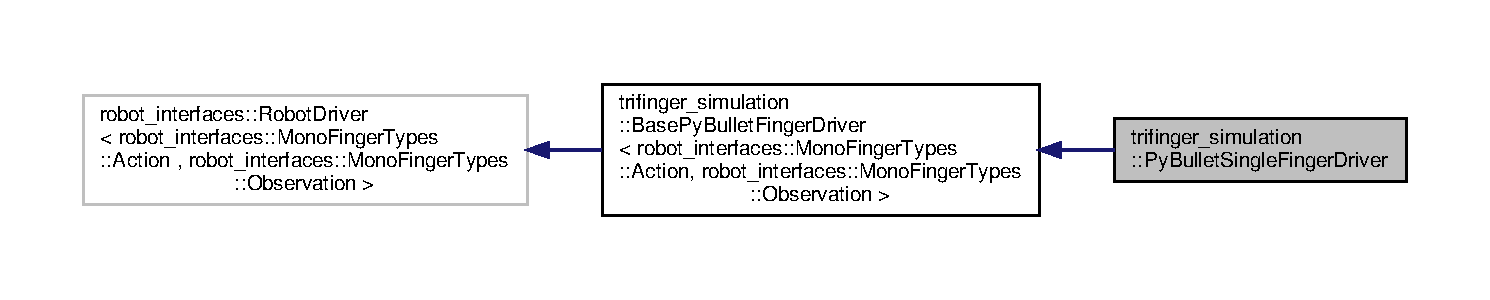
\includegraphics[width=350pt]{classtrifinger__simulation_1_1PyBulletSingleFingerDriver__inherit__graph}
\end{center}
\end{figure}


Collaboration diagram for trifinger\+\_\+simulation\+:\+:Py\+Bullet\+Single\+Finger\+Driver\+:
\nopagebreak
\begin{figure}[H]
\begin{center}
\leavevmode
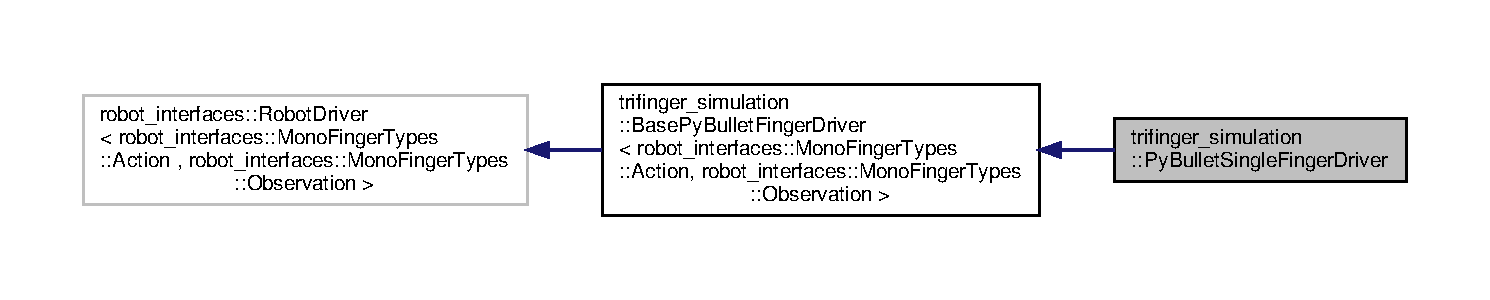
\includegraphics[width=350pt]{classtrifinger__simulation_1_1PyBulletSingleFingerDriver__coll__graph}
\end{center}
\end{figure}
\subsection*{Public Member Functions}
\begin{DoxyCompactItemize}
\item 
\mbox{\Hypertarget{classtrifinger__simulation_1_1PyBulletSingleFingerDriver_a5ed94f4f994ebdc286e6472095d3b623}\label{classtrifinger__simulation_1_1PyBulletSingleFingerDriver_a5ed94f4f994ebdc286e6472095d3b623}} 
void {\bfseries initialize} () override
\end{DoxyCompactItemize}
\subsection*{Additional Inherited Members}


\subsection{Detailed Description}
py\+Bullet driver for the single Finger. 

The documentation for this class was generated from the following file\+:\begin{DoxyCompactItemize}
\item 
include/trifinger\+\_\+simulation/\hyperlink{pybullet__driver_8hpp}{pybullet\+\_\+driver.\+hpp}\end{DoxyCompactItemize}

\hypertarget{classtrifinger__simulation_1_1PyBulletTriFingerDriver}{}\section{trifinger\+\_\+simulation\+:\+:Py\+Bullet\+Tri\+Finger\+Driver Class Reference}
\label{classtrifinger__simulation_1_1PyBulletTriFingerDriver}\index{trifinger\+\_\+simulation\+::\+Py\+Bullet\+Tri\+Finger\+Driver@{trifinger\+\_\+simulation\+::\+Py\+Bullet\+Tri\+Finger\+Driver}}


py\+Bullet driver for the Tri\+Finger  




{\ttfamily \#include $<$pybullet\+\_\+driver.\+hpp$>$}



Inheritance diagram for trifinger\+\_\+simulation\+:\+:Py\+Bullet\+Tri\+Finger\+Driver\+:
\nopagebreak
\begin{figure}[H]
\begin{center}
\leavevmode
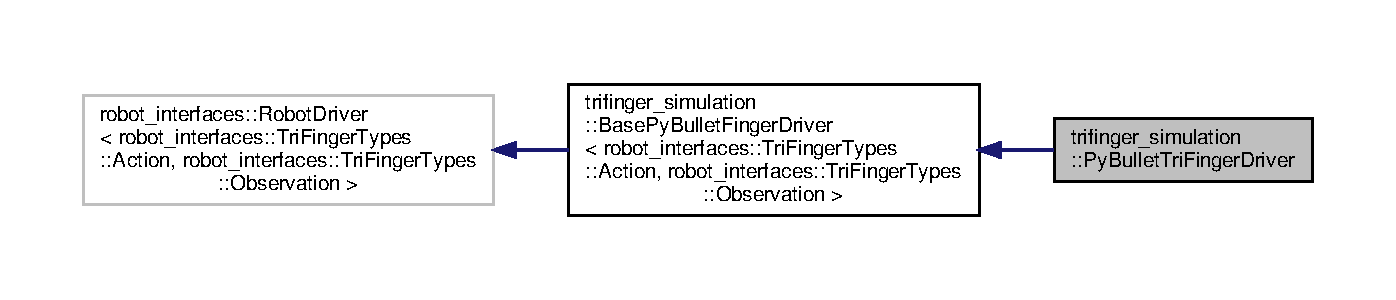
\includegraphics[width=350pt]{classtrifinger__simulation_1_1PyBulletTriFingerDriver__inherit__graph}
\end{center}
\end{figure}


Collaboration diagram for trifinger\+\_\+simulation\+:\+:Py\+Bullet\+Tri\+Finger\+Driver\+:
\nopagebreak
\begin{figure}[H]
\begin{center}
\leavevmode
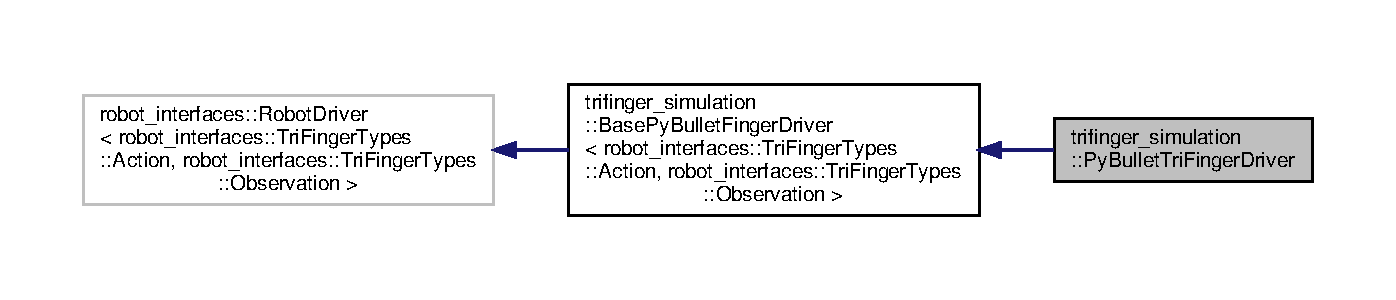
\includegraphics[width=350pt]{classtrifinger__simulation_1_1PyBulletTriFingerDriver__coll__graph}
\end{center}
\end{figure}
\subsection*{Public Member Functions}
\begin{DoxyCompactItemize}
\item 
\mbox{\Hypertarget{classtrifinger__simulation_1_1PyBulletTriFingerDriver_a15f298c6ccf4ac825880e801b3c4db2c}\label{classtrifinger__simulation_1_1PyBulletTriFingerDriver_a15f298c6ccf4ac825880e801b3c4db2c}} 
void {\bfseries initialize} () override
\end{DoxyCompactItemize}
\subsection*{Additional Inherited Members}


\subsection{Detailed Description}
py\+Bullet driver for the Tri\+Finger 

The documentation for this class was generated from the following file\+:\begin{DoxyCompactItemize}
\item 
include/trifinger\+\_\+simulation/\hyperlink{pybullet__driver_8hpp}{pybullet\+\_\+driver.\+hpp}\end{DoxyCompactItemize}

\hypertarget{classevaluate__policy_1_1RandomPolicy}{}\section{evaluate\+\_\+policy.\+Random\+Policy Class Reference}
\label{classevaluate__policy_1_1RandomPolicy}\index{evaluate\+\_\+policy.\+Random\+Policy@{evaluate\+\_\+policy.\+Random\+Policy}}


Dummy policy which uses random actions.  


\subsection*{Public Member Functions}
\begin{DoxyCompactItemize}
\item 
\mbox{\Hypertarget{classevaluate__policy_1_1RandomPolicy_ab17a5904a79a5ff6a9606ce9171af7ee}\label{classevaluate__policy_1_1RandomPolicy_ab17a5904a79a5ff6a9606ce9171af7ee}} 
def {\bfseries \+\_\+\+\_\+init\+\_\+\+\_\+} (self, action\+\_\+space)
\item 
\mbox{\Hypertarget{classevaluate__policy_1_1RandomPolicy_ae1e2478222b2e6b00a68b7973a60ebe1}\label{classevaluate__policy_1_1RandomPolicy_ae1e2478222b2e6b00a68b7973a60ebe1}} 
def {\bfseries predict} (self, observation)
\item 
\mbox{\Hypertarget{classevaluate__policy_1_1RandomPolicy_ab17a5904a79a5ff6a9606ce9171af7ee}\label{classevaluate__policy_1_1RandomPolicy_ab17a5904a79a5ff6a9606ce9171af7ee}} 
def {\bfseries \+\_\+\+\_\+init\+\_\+\+\_\+} (self, action\+\_\+space)
\item 
\mbox{\Hypertarget{classevaluate__policy_1_1RandomPolicy_ae1e2478222b2e6b00a68b7973a60ebe1}\label{classevaluate__policy_1_1RandomPolicy_ae1e2478222b2e6b00a68b7973a60ebe1}} 
def {\bfseries predict} (self, observation)
\end{DoxyCompactItemize}
\subsection*{Public Attributes}
\begin{DoxyCompactItemize}
\item 
\mbox{\Hypertarget{classevaluate__policy_1_1RandomPolicy_adfcfaa59da2ab4aed58a1cd95f99b7d8}\label{classevaluate__policy_1_1RandomPolicy_adfcfaa59da2ab4aed58a1cd95f99b7d8}} 
{\bfseries action\+\_\+space}
\end{DoxyCompactItemize}


\subsection{Detailed Description}
Dummy policy which uses random actions. 



The documentation for this class was generated from the following file\+:\begin{DoxyCompactItemize}
\item 
example/evaluate\+\_\+policy.\+py\end{DoxyCompactItemize}

\hypertarget{classdemo__random__policy_1_1RandomPolicy}{}\section{demo\+\_\+random\+\_\+policy.\+Random\+Policy Class Reference}
\label{classdemo__random__policy_1_1RandomPolicy}\index{demo\+\_\+random\+\_\+policy.\+Random\+Policy@{demo\+\_\+random\+\_\+policy.\+Random\+Policy}}


Dummy policy which uses random actions.  


\subsection*{Public Member Functions}
\begin{DoxyCompactItemize}
\item 
\mbox{\Hypertarget{classdemo__random__policy_1_1RandomPolicy_acf3ead594e7856f4a21854613280e6e0}\label{classdemo__random__policy_1_1RandomPolicy_acf3ead594e7856f4a21854613280e6e0}} 
def {\bfseries \+\_\+\+\_\+init\+\_\+\+\_\+} (self, action\+\_\+space)
\item 
\mbox{\Hypertarget{classdemo__random__policy_1_1RandomPolicy_a2d594da9acda1a454d4986f5a0017dbe}\label{classdemo__random__policy_1_1RandomPolicy_a2d594da9acda1a454d4986f5a0017dbe}} 
def {\bfseries predict} (self, observation)
\end{DoxyCompactItemize}
\subsection*{Public Attributes}
\begin{DoxyCompactItemize}
\item 
\mbox{\Hypertarget{classdemo__random__policy_1_1RandomPolicy_a97882a0e59c4258e6001128b9f194c21}\label{classdemo__random__policy_1_1RandomPolicy_a97882a0e59c4258e6001128b9f194c21}} 
{\bfseries action\+\_\+space}
\end{DoxyCompactItemize}


\subsection{Detailed Description}
Dummy policy which uses random actions. 



The documentation for this class was generated from the following file\+:\begin{DoxyCompactItemize}
\item 
demos/demo\+\_\+random\+\_\+policy.\+py\end{DoxyCompactItemize}

\hypertarget{classtrifinger__simulation_1_1real__finger_1_1RealFinger}{}\section{trifinger\+\_\+simulation.\+real\+\_\+finger.\+Real\+Finger Class Reference}
\label{classtrifinger__simulation_1_1real__finger_1_1RealFinger}\index{trifinger\+\_\+simulation.\+real\+\_\+finger.\+Real\+Finger@{trifinger\+\_\+simulation.\+real\+\_\+finger.\+Real\+Finger}}
\subsection*{Public Member Functions}
\begin{DoxyCompactItemize}
\item 
def \hyperlink{classtrifinger__simulation_1_1real__finger_1_1RealFinger_ac439b679344398a9ea05e8dbe2b4d9e4}{\+\_\+\+\_\+init\+\_\+\+\_\+} (self, finger\+\_\+type, finger\+\_\+config\+\_\+suffix, enable\+\_\+visualization=False)
\begin{DoxyCompactList}\small\item\em Constructor, initializes the physical world we will work in. \end{DoxyCompactList}\item 
\mbox{\Hypertarget{classtrifinger__simulation_1_1real__finger_1_1RealFinger_a88c73a72ad0f45cb379bc72394183fbf}\label{classtrifinger__simulation_1_1real__finger_1_1RealFinger_a88c73a72ad0f45cb379bc72394183fbf}} 
def {\bfseries append\+\_\+desired\+\_\+action} (self, action)
\item 
def \hyperlink{classtrifinger__simulation_1_1real__finger_1_1RealFinger_a5e10f8a9627376f072ad2ea64ecdd361}{get\+\_\+observation} (self, time\+\_\+index)
\begin{DoxyCompactList}\small\item\em Get the observation from the robot at a specified time\+\_\+index. \end{DoxyCompactList}\item 
\mbox{\Hypertarget{classtrifinger__simulation_1_1real__finger_1_1RealFinger_ac6d714de5c42486c3bfbc745c8370a6f}\label{classtrifinger__simulation_1_1real__finger_1_1RealFinger_ac6d714de5c42486c3bfbc745c8370a6f}} 
def {\bfseries reset\+\_\+finger} (self, joint\+\_\+positions)
\end{DoxyCompactItemize}
\subsection*{Public Attributes}
\begin{DoxyCompactItemize}
\item 
\mbox{\Hypertarget{classtrifinger__simulation_1_1real__finger_1_1RealFinger_ac89964cae309710fc2dda9a5db859e19}\label{classtrifinger__simulation_1_1real__finger_1_1RealFinger_ac89964cae309710fc2dda9a5db859e19}} 
{\bfseries simulator}
\item 
\mbox{\Hypertarget{classtrifinger__simulation_1_1real__finger_1_1RealFinger_a202d50223d0724b8478a8a675b881fc1}\label{classtrifinger__simulation_1_1real__finger_1_1RealFinger_a202d50223d0724b8478a8a675b881fc1}} 
{\bfseries real\+\_\+finger\+\_\+backend}
\item 
\mbox{\Hypertarget{classtrifinger__simulation_1_1real__finger_1_1RealFinger_a4d76b5b82c37f49075e0e84177b27967}\label{classtrifinger__simulation_1_1real__finger_1_1RealFinger_a4d76b5b82c37f49075e0e84177b27967}} 
{\bfseries robot}
\item 
\mbox{\Hypertarget{classtrifinger__simulation_1_1real__finger_1_1RealFinger_ab9c79d41e501ae1e9478cf5417d23334}\label{classtrifinger__simulation_1_1real__finger_1_1RealFinger_ab9c79d41e501ae1e9478cf5417d23334}} 
{\bfseries Action}
\end{DoxyCompactItemize}


\subsection{Constructor \& Destructor Documentation}
\mbox{\Hypertarget{classtrifinger__simulation_1_1real__finger_1_1RealFinger_ac439b679344398a9ea05e8dbe2b4d9e4}\label{classtrifinger__simulation_1_1real__finger_1_1RealFinger_ac439b679344398a9ea05e8dbe2b4d9e4}} 
\index{trifinger\+\_\+simulation\+::real\+\_\+finger\+::\+Real\+Finger@{trifinger\+\_\+simulation\+::real\+\_\+finger\+::\+Real\+Finger}!\+\_\+\+\_\+init\+\_\+\+\_\+@{\+\_\+\+\_\+init\+\_\+\+\_\+}}
\index{\+\_\+\+\_\+init\+\_\+\+\_\+@{\+\_\+\+\_\+init\+\_\+\+\_\+}!trifinger\+\_\+simulation\+::real\+\_\+finger\+::\+Real\+Finger@{trifinger\+\_\+simulation\+::real\+\_\+finger\+::\+Real\+Finger}}
\subsubsection{\texorpdfstring{\+\_\+\+\_\+init\+\_\+\+\_\+()}{\_\_init\_\_()}}
{\footnotesize\ttfamily def trifinger\+\_\+simulation.\+real\+\_\+finger.\+Real\+Finger.\+\_\+\+\_\+init\+\_\+\+\_\+ (\begin{DoxyParamCaption}\item[{}]{self,  }\item[{}]{finger\+\_\+type,  }\item[{}]{finger\+\_\+config\+\_\+suffix,  }\item[{}]{enable\+\_\+visualization = {\ttfamily False} }\end{DoxyParamCaption})}



Constructor, initializes the physical world we will work in. 


\begin{DoxyParams}{Parameters}
{\em finger\+\_\+type} & Name of the finger type. In order to get a list of the valid finger types, call \+:meth\+:{\ttfamily .finger\+\_\+types\+\_\+data.\+get\+\_\+valid\+\_\+finger\+\_\+types}. \\
\hline
{\em finger\+\_\+config\+\_\+suffix} & ID of the finger that is used. Has to be one of \mbox{[}0, 120, 240\mbox{]}. This is only if a single finger is to be used on any of the robots, and is ignored otherwise. enable\+\_\+visualization (bool, optional)\+: Set to \textquotesingle{}True\textquotesingle{} to run a G\+UI for visualization. This uses py\+Bullet but only for visualization, i.\+e. the state of the simulation is constantly set to match the one of the real robot. \\
\hline
\end{DoxyParams}


\subsection{Member Function Documentation}
\mbox{\Hypertarget{classtrifinger__simulation_1_1real__finger_1_1RealFinger_a5e10f8a9627376f072ad2ea64ecdd361}\label{classtrifinger__simulation_1_1real__finger_1_1RealFinger_a5e10f8a9627376f072ad2ea64ecdd361}} 
\index{trifinger\+\_\+simulation\+::real\+\_\+finger\+::\+Real\+Finger@{trifinger\+\_\+simulation\+::real\+\_\+finger\+::\+Real\+Finger}!get\+\_\+observation@{get\+\_\+observation}}
\index{get\+\_\+observation@{get\+\_\+observation}!trifinger\+\_\+simulation\+::real\+\_\+finger\+::\+Real\+Finger@{trifinger\+\_\+simulation\+::real\+\_\+finger\+::\+Real\+Finger}}
\subsubsection{\texorpdfstring{get\+\_\+observation()}{get\_observation()}}
{\footnotesize\ttfamily def trifinger\+\_\+simulation.\+real\+\_\+finger.\+Real\+Finger.\+get\+\_\+observation (\begin{DoxyParamCaption}\item[{}]{self,  }\item[{}]{time\+\_\+index }\end{DoxyParamCaption})}



Get the observation from the robot at a specified time\+\_\+index. 


\begin{DoxyParams}{Parameters}
{\em time\+\_\+index} & the time\+\_\+index at which the observation is \\
\hline
{\em needed} & \\
\hline
\end{DoxyParams}
\begin{DoxyReturn}{Returns}


observation the corresponding observation 
\end{DoxyReturn}


The documentation for this class was generated from the following file\+:\begin{DoxyCompactItemize}
\item 
python/trifinger\+\_\+simulation/real\+\_\+finger.\+py\end{DoxyCompactItemize}

\hypertarget{classtrifinger__simulation_1_1sim__finger_1_1SimFinger}{}\section{trifinger\+\_\+simulation.\+sim\+\_\+finger.\+Sim\+Finger Class Reference}
\label{classtrifinger__simulation_1_1sim__finger_1_1SimFinger}\index{trifinger\+\_\+simulation.\+sim\+\_\+finger.\+Sim\+Finger@{trifinger\+\_\+simulation.\+sim\+\_\+finger.\+Sim\+Finger}}
\subsection*{Public Member Functions}
\begin{DoxyCompactItemize}
\item 
def \hyperlink{classtrifinger__simulation_1_1sim__finger_1_1SimFinger_a3bf64d6f490e704bfe3626bd0125451a}{\+\_\+\+\_\+init\+\_\+\+\_\+} (self, \hyperlink{classtrifinger__simulation_1_1sim__finger_1_1SimFinger_a34b39b76cad22883bee483aed5d79b09}{finger\+\_\+type}, time\+\_\+step=0.\+004, enable\+\_\+visualization=False)
\begin{DoxyCompactList}\small\item\em Constructor, initializes the physical world we will work in. \end{DoxyCompactList}\item 
def \hyperlink{classtrifinger__simulation_1_1sim__finger_1_1SimFinger_ad5b6ac0efef02c0f3334a44e79bd4413}{Action} (self, torque=None, position=None)
\begin{DoxyCompactList}\small\item\em Fill in the fields of the action structure. \end{DoxyCompactList}\item 
\mbox{\Hypertarget{classtrifinger__simulation_1_1sim__finger_1_1SimFinger_ad02a3dc3f4a3c824fec864ce1d1464e9}\label{classtrifinger__simulation_1_1sim__finger_1_1SimFinger_ad02a3dc3f4a3c824fec864ce1d1464e9}} 
def {\bfseries get\+\_\+observation} (self, t)
\item 
\mbox{\Hypertarget{classtrifinger__simulation_1_1sim__finger_1_1SimFinger_a71650072f6feecbc2c78a16cfa12ee77}\label{classtrifinger__simulation_1_1sim__finger_1_1SimFinger_a71650072f6feecbc2c78a16cfa12ee77}} 
def {\bfseries append\+\_\+desired\+\_\+action} (self, action)
\item 
def \hyperlink{classtrifinger__simulation_1_1sim__finger_1_1SimFinger_a1a808eb19a1a9a13a4c0fe4f2d07d26c}{get\+\_\+desired\+\_\+action} (self, t)
\begin{DoxyCompactList}\small\item\em Get the desired action of time step \textquotesingle{}t\textquotesingle{}. \end{DoxyCompactList}\item 
def \hyperlink{classtrifinger__simulation_1_1sim__finger_1_1SimFinger_a1aa1717c3ea9c3d78659360e64246544}{get\+\_\+applied\+\_\+action} (self, t)
\begin{DoxyCompactList}\small\item\em Get the actually applied action of time step \textquotesingle{}t\textquotesingle{}. \end{DoxyCompactList}\item 
def \hyperlink{classtrifinger__simulation_1_1sim__finger_1_1SimFinger_a7836fb9b5deacefa636afcea7b9639d7}{get\+\_\+timestamp\+\_\+ms} (self, t)
\begin{DoxyCompactList}\small\item\em Get timestamp of time step \textquotesingle{}t\textquotesingle{}. \end{DoxyCompactList}\item 
def \hyperlink{classtrifinger__simulation_1_1sim__finger_1_1SimFinger_a26ba218495f7bb5c1615184070100df5}{get\+\_\+current\+\_\+timeindex} (self)
\begin{DoxyCompactList}\small\item\em Get the current time index. \end{DoxyCompactList}\item 
\mbox{\Hypertarget{classtrifinger__simulation_1_1sim__finger_1_1SimFinger_a791e4675bdcbb97ecdfb7e27c407e603}\label{classtrifinger__simulation_1_1sim__finger_1_1SimFinger_a791e4675bdcbb97ecdfb7e27c407e603}} 
def {\bfseries reset\+\_\+finger\+\_\+positions\+\_\+and\+\_\+velocities} (self, joint\+\_\+positions, joint\+\_\+velocities=None)
\item 
def \hyperlink{classtrifinger__simulation_1_1sim__finger_1_1SimFinger_acad7e2ed039c444081cb287d7ba33428}{\+\_\+\+\_\+del\+\_\+\+\_\+} (self)
\begin{DoxyCompactList}\small\item\em Clean up. \end{DoxyCompactList}\end{DoxyCompactItemize}
\subsection*{Public Attributes}
\begin{DoxyCompactItemize}
\item 
\hyperlink{classtrifinger__simulation_1_1sim__finger_1_1SimFinger_a34b39b76cad22883bee483aed5d79b09}{finger\+\_\+type}
\begin{DoxyCompactList}\small\item\em Name of the finger type. \end{DoxyCompactList}\item 
\mbox{\Hypertarget{classtrifinger__simulation_1_1sim__finger_1_1SimFinger_ab19ef3bd876d915d8e5ffd601f2a9b0a}\label{classtrifinger__simulation_1_1sim__finger_1_1SimFinger_ab19ef3bd876d915d8e5ffd601f2a9b0a}} 
{\bfseries number\+\_\+of\+\_\+fingers}
\item 
\mbox{\Hypertarget{classtrifinger__simulation_1_1sim__finger_1_1SimFinger_a9996b39168c94660f4035bea36501a69}\label{classtrifinger__simulation_1_1sim__finger_1_1SimFinger_a9996b39168c94660f4035bea36501a69}} 
{\bfseries time\+\_\+step\+\_\+s}
\item 
\mbox{\Hypertarget{classtrifinger__simulation_1_1sim__finger_1_1SimFinger_a6a6f010aacbd68321eb378bea9dd55fd}\label{classtrifinger__simulation_1_1sim__finger_1_1SimFinger_a6a6f010aacbd68321eb378bea9dd55fd}} 
{\bfseries position\+\_\+gains}
\item 
\mbox{\Hypertarget{classtrifinger__simulation_1_1sim__finger_1_1SimFinger_a1167d3f99f5e1900722838363fe584ec}\label{classtrifinger__simulation_1_1sim__finger_1_1SimFinger_a1167d3f99f5e1900722838363fe584ec}} 
{\bfseries velocity\+\_\+gains}
\item 
\mbox{\Hypertarget{classtrifinger__simulation_1_1sim__finger_1_1SimFinger_aab6de2707772291150a0f4806457cb74}\label{classtrifinger__simulation_1_1sim__finger_1_1SimFinger_aab6de2707772291150a0f4806457cb74}} 
{\bfseries safety\+\_\+kd}
\item 
\mbox{\Hypertarget{classtrifinger__simulation_1_1sim__finger_1_1SimFinger_ac00e9a11b88c49ce9ea4fdd57c885278}\label{classtrifinger__simulation_1_1sim__finger_1_1SimFinger_ac00e9a11b88c49ce9ea4fdd57c885278}} 
{\bfseries max\+\_\+motor\+\_\+torque}
\item 
\mbox{\Hypertarget{classtrifinger__simulation_1_1sim__finger_1_1SimFinger_a37cfc20c54ff7528989bd4cc6093ae17}\label{classtrifinger__simulation_1_1sim__finger_1_1SimFinger_a37cfc20c54ff7528989bd4cc6093ae17}} 
{\bfseries pinocchio\+\_\+utils}
\item 
\mbox{\Hypertarget{classtrifinger__simulation_1_1sim__finger_1_1SimFinger_a294b9db831667417f369e40215edd8b4}\label{classtrifinger__simulation_1_1sim__finger_1_1SimFinger_a294b9db831667417f369e40215edd8b4}} 
{\bfseries link\+\_\+names}
\item 
\mbox{\Hypertarget{classtrifinger__simulation_1_1sim__finger_1_1SimFinger_af663fe142856d344fdbb58f22c37efa7}\label{classtrifinger__simulation_1_1sim__finger_1_1SimFinger_af663fe142856d344fdbb58f22c37efa7}} 
{\bfseries tip\+\_\+link\+\_\+names}
\item 
\mbox{\Hypertarget{classtrifinger__simulation_1_1sim__finger_1_1SimFinger_a27c0a7ebff95df779c68978b9206658e}\label{classtrifinger__simulation_1_1sim__finger_1_1SimFinger_a27c0a7ebff95df779c68978b9206658e}} 
{\bfseries robot\+\_\+properties\+\_\+path}
\item 
\mbox{\Hypertarget{classtrifinger__simulation_1_1sim__finger_1_1SimFinger_a75ccecd477ea9c4ce8345bf25ed020e4}\label{classtrifinger__simulation_1_1sim__finger_1_1SimFinger_a75ccecd477ea9c4ce8345bf25ed020e4}} 
{\bfseries finger\+\_\+urdf\+\_\+path}
\item 
\mbox{\Hypertarget{classtrifinger__simulation_1_1sim__finger_1_1SimFinger_adcb28714dbfeaa21c2b7e3e6daa52628}\label{classtrifinger__simulation_1_1sim__finger_1_1SimFinger_adcb28714dbfeaa21c2b7e3e6daa52628}} 
{\bfseries finger\+\_\+id}
\item 
\mbox{\Hypertarget{classtrifinger__simulation_1_1sim__finger_1_1SimFinger_a78e2ef01f3c0a6155f145c1631768fcc}\label{classtrifinger__simulation_1_1sim__finger_1_1SimFinger_a78e2ef01f3c0a6155f145c1631768fcc}} 
{\bfseries pybullet\+\_\+link\+\_\+indices}
\item 
\mbox{\Hypertarget{classtrifinger__simulation_1_1sim__finger_1_1SimFinger_adf3ff8525662c2f4842c6d4b2a49fa6a}\label{classtrifinger__simulation_1_1sim__finger_1_1SimFinger_adf3ff8525662c2f4842c6d4b2a49fa6a}} 
{\bfseries pybullet\+\_\+tip\+\_\+link\+\_\+indices}
\item 
\mbox{\Hypertarget{classtrifinger__simulation_1_1sim__finger_1_1SimFinger_a9420370026aa26d65ca47de77548ec0e}\label{classtrifinger__simulation_1_1sim__finger_1_1SimFinger_a9420370026aa26d65ca47de77548ec0e}} 
{\bfseries pybullet\+\_\+joint\+\_\+indices}
\end{DoxyCompactItemize}
\subsection*{Private Member Functions}
\begin{DoxyCompactItemize}
\item 
def \hyperlink{classtrifinger__simulation_1_1sim__finger_1_1SimFinger_afa4a964d02c90e36da1adae854f79b2e}{\+\_\+get\+\_\+latest\+\_\+observation} (self)
\begin{DoxyCompactList}\small\item\em Get observation of the current state. \end{DoxyCompactList}\item 
def \hyperlink{classtrifinger__simulation_1_1sim__finger_1_1SimFinger_a05f4dff6e5d524a8c86f27bc76f2199e}{\+\_\+set\+\_\+desired\+\_\+action} (self, desired\+\_\+action)
\begin{DoxyCompactList}\small\item\em Set the given action after performing safety checks. \end{DoxyCompactList}\item 
\mbox{\Hypertarget{classtrifinger__simulation_1_1sim__finger_1_1SimFinger_a2c7322d4a75101b6947c8b6d3004e3b5}\label{classtrifinger__simulation_1_1sim__finger_1_1SimFinger_a2c7322d4a75101b6947c8b6d3004e3b5}} 
def \hyperlink{classtrifinger__simulation_1_1sim__finger_1_1SimFinger_a2c7322d4a75101b6947c8b6d3004e3b5}{\+\_\+step\+\_\+simulation} (self)
\begin{DoxyCompactList}\small\item\em Step the simulation to go to the next world state. \end{DoxyCompactList}\item 
def \hyperlink{classtrifinger__simulation_1_1sim__finger_1_1SimFinger_a946035313313f8068a568360f53cfa48}{\+\_\+disconnect\+\_\+from\+\_\+pybullet} (self)
\begin{DoxyCompactList}\small\item\em Disconnect from the simulation. \end{DoxyCompactList}\item 
\mbox{\Hypertarget{classtrifinger__simulation_1_1sim__finger_1_1SimFinger_a9fbb93e4c2ad2f6f22786b4930fb1ceb}\label{classtrifinger__simulation_1_1sim__finger_1_1SimFinger_a9fbb93e4c2ad2f6f22786b4930fb1ceb}} 
def {\bfseries \+\_\+\+\_\+set\+\_\+pybullet\+\_\+motor\+\_\+torques} (self, motor\+\_\+torques)
\item 
\mbox{\Hypertarget{classtrifinger__simulation_1_1sim__finger_1_1SimFinger_a5ced4773d25b0160f8ae503c97647348}\label{classtrifinger__simulation_1_1sim__finger_1_1SimFinger_a5ced4773d25b0160f8ae503c97647348}} 
def {\bfseries \+\_\+\+\_\+safety\+\_\+check\+\_\+torques} (self, desired\+\_\+torques)
\item 
\mbox{\Hypertarget{classtrifinger__simulation_1_1sim__finger_1_1SimFinger_a089d0071570e20fec80293c13b3cc47d}\label{classtrifinger__simulation_1_1sim__finger_1_1SimFinger_a089d0071570e20fec80293c13b3cc47d}} 
def {\bfseries \+\_\+\+\_\+compute\+\_\+pd\+\_\+control\+\_\+torques} (self, joint\+\_\+positions, kp=None, kd=None)
\item 
\mbox{\Hypertarget{classtrifinger__simulation_1_1sim__finger_1_1SimFinger_a31c82455c5345ff47a0e7ce1bc22df13}\label{classtrifinger__simulation_1_1sim__finger_1_1SimFinger_a31c82455c5345ff47a0e7ce1bc22df13}} 
def \hyperlink{classtrifinger__simulation_1_1sim__finger_1_1SimFinger_a31c82455c5345ff47a0e7ce1bc22df13}{\+\_\+\+\_\+validate\+\_\+time\+\_\+index} (self, t)
\begin{DoxyCompactList}\small\item\em Raise error if t does not match with self.\+\_\+t. \end{DoxyCompactList}\item 
\mbox{\Hypertarget{classtrifinger__simulation_1_1sim__finger_1_1SimFinger_a3ce491d53c13c11b3db5c8b5846570b2}\label{classtrifinger__simulation_1_1sim__finger_1_1SimFinger_a3ce491d53c13c11b3db5c8b5846570b2}} 
def \hyperlink{classtrifinger__simulation_1_1sim__finger_1_1SimFinger_a3ce491d53c13c11b3db5c8b5846570b2}{\+\_\+\+\_\+create\+\_\+link\+\_\+lists} (self)
\begin{DoxyCompactList}\small\item\em Initialize lists of link/joint names depending on which robot is used. \end{DoxyCompactList}\item 
\mbox{\Hypertarget{classtrifinger__simulation_1_1sim__finger_1_1SimFinger_a4c3d2e479821ee10759db74151308932}\label{classtrifinger__simulation_1_1sim__finger_1_1SimFinger_a4c3d2e479821ee10759db74151308932}} 
def {\bfseries \+\_\+\+\_\+setup\+\_\+pybullet\+\_\+simulation} (self)
\item 
\mbox{\Hypertarget{classtrifinger__simulation_1_1sim__finger_1_1SimFinger_a8942bdfacf8a1c9750422f95cc955bf7}\label{classtrifinger__simulation_1_1sim__finger_1_1SimFinger_a8942bdfacf8a1c9750422f95cc955bf7}} 
def {\bfseries \+\_\+\+\_\+set\+\_\+pybullet\+\_\+params} (self)
\item 
\mbox{\Hypertarget{classtrifinger__simulation_1_1sim__finger_1_1SimFinger_a0a10efd7b04307ad71fbaf45ec94a6fe}\label{classtrifinger__simulation_1_1sim__finger_1_1SimFinger_a0a10efd7b04307ad71fbaf45ec94a6fe}} 
def {\bfseries \+\_\+\+\_\+disable\+\_\+pybullet\+\_\+velocity\+\_\+control} (self)
\item 
\mbox{\Hypertarget{classtrifinger__simulation_1_1sim__finger_1_1SimFinger_abc4c06d8b54077f9494ae9fd78014bee}\label{classtrifinger__simulation_1_1sim__finger_1_1SimFinger_abc4c06d8b54077f9494ae9fd78014bee}} 
def \hyperlink{classtrifinger__simulation_1_1sim__finger_1_1SimFinger_abc4c06d8b54077f9494ae9fd78014bee}{\+\_\+\+\_\+set\+\_\+urdf\+\_\+path} (self)
\begin{DoxyCompactList}\small\item\em Sets the paths for the U\+R\+D\+Fs to use depending upon the finger type. \end{DoxyCompactList}\item 
\mbox{\Hypertarget{classtrifinger__simulation_1_1sim__finger_1_1SimFinger_afb59a872dc92feaad5d292e69af4efd5}\label{classtrifinger__simulation_1_1sim__finger_1_1SimFinger_afb59a872dc92feaad5d292e69af4efd5}} 
def \hyperlink{classtrifinger__simulation_1_1sim__finger_1_1SimFinger_afb59a872dc92feaad5d292e69af4efd5}{\+\_\+\+\_\+load\+\_\+robot\+\_\+urdf} (self)
\begin{DoxyCompactList}\small\item\em Load the single/trifinger model from the corresponding urdf. \end{DoxyCompactList}\item 
def \hyperlink{classtrifinger__simulation_1_1sim__finger_1_1SimFinger_ae5b729d7973f90ad9511c4581d454a52}{\+\_\+\+\_\+load\+\_\+stage} (self, high\+\_\+border=True)
\begin{DoxyCompactList}\small\item\em Create the stage (table and boundary). \end{DoxyCompactList}\end{DoxyCompactItemize}
\subsection*{Static Private Member Functions}
\begin{DoxyCompactItemize}
\item 
\mbox{\Hypertarget{classtrifinger__simulation_1_1sim__finger_1_1SimFinger_ae96f1cab7a32d2133b60fca99d2cb783}\label{classtrifinger__simulation_1_1sim__finger_1_1SimFinger_ae96f1cab7a32d2133b60fca99d2cb783}} 
def {\bfseries \+\_\+\+\_\+connect\+\_\+to\+\_\+pybullet} (enable\+\_\+visualization)
\end{DoxyCompactItemize}
\subsection*{Private Attributes}
\begin{DoxyCompactItemize}
\item 
\mbox{\Hypertarget{classtrifinger__simulation_1_1sim__finger_1_1SimFinger_a782e9d0d2a0bc5ad87ad7a826d8f5e40}\label{classtrifinger__simulation_1_1sim__finger_1_1SimFinger_a782e9d0d2a0bc5ad87ad7a826d8f5e40}} 
{\bfseries \+\_\+t}
\item 
\mbox{\Hypertarget{classtrifinger__simulation_1_1sim__finger_1_1SimFinger_a37d29f33684c35e5c1e06456145d7308}\label{classtrifinger__simulation_1_1sim__finger_1_1SimFinger_a37d29f33684c35e5c1e06456145d7308}} 
{\bfseries \+\_\+desired\+\_\+action\+\_\+t}
\item 
\mbox{\Hypertarget{classtrifinger__simulation_1_1sim__finger_1_1SimFinger_a4050222bee7230c4a2529fddf36dd9fb}\label{classtrifinger__simulation_1_1sim__finger_1_1SimFinger_a4050222bee7230c4a2529fddf36dd9fb}} 
{\bfseries \+\_\+applied\+\_\+action\+\_\+t}
\item 
\mbox{\Hypertarget{classtrifinger__simulation_1_1sim__finger_1_1SimFinger_ab21731192738ee73f1a04a5e9663e2c1}\label{classtrifinger__simulation_1_1sim__finger_1_1SimFinger_ab21731192738ee73f1a04a5e9663e2c1}} 
{\bfseries \+\_\+observation\+\_\+t}
\end{DoxyCompactItemize}


\subsection{Constructor \& Destructor Documentation}
\mbox{\Hypertarget{classtrifinger__simulation_1_1sim__finger_1_1SimFinger_a3bf64d6f490e704bfe3626bd0125451a}\label{classtrifinger__simulation_1_1sim__finger_1_1SimFinger_a3bf64d6f490e704bfe3626bd0125451a}} 
\index{trifinger\+\_\+simulation\+::sim\+\_\+finger\+::\+Sim\+Finger@{trifinger\+\_\+simulation\+::sim\+\_\+finger\+::\+Sim\+Finger}!\+\_\+\+\_\+init\+\_\+\+\_\+@{\+\_\+\+\_\+init\+\_\+\+\_\+}}
\index{\+\_\+\+\_\+init\+\_\+\+\_\+@{\+\_\+\+\_\+init\+\_\+\+\_\+}!trifinger\+\_\+simulation\+::sim\+\_\+finger\+::\+Sim\+Finger@{trifinger\+\_\+simulation\+::sim\+\_\+finger\+::\+Sim\+Finger}}
\subsubsection{\texorpdfstring{\+\_\+\+\_\+init\+\_\+\+\_\+()}{\_\_init\_\_()}}
{\footnotesize\ttfamily def trifinger\+\_\+simulation.\+sim\+\_\+finger.\+Sim\+Finger.\+\_\+\+\_\+init\+\_\+\+\_\+ (\begin{DoxyParamCaption}\item[{}]{self,  }\item[{}]{finger\+\_\+type,  }\item[{}]{time\+\_\+step = {\ttfamily 0.004},  }\item[{}]{enable\+\_\+visualization = {\ttfamily False} }\end{DoxyParamCaption})}



Constructor, initializes the physical world we will work in. 


\begin{DoxyParams}{Parameters}
{\em finger\+\_\+type} & See \+:attr\+:{\ttfamily finger\+\_\+type} \\
\hline
{\em time\+\_\+step} & See \+:attr\+:{\ttfamily time\+\_\+step} \\
\hline
{\em enable\+\_\+visualization} & See \+:attr\+:{\ttfamily enable\+\_\+visualization} \\
\hline
\end{DoxyParams}
\mbox{\Hypertarget{classtrifinger__simulation_1_1sim__finger_1_1SimFinger_acad7e2ed039c444081cb287d7ba33428}\label{classtrifinger__simulation_1_1sim__finger_1_1SimFinger_acad7e2ed039c444081cb287d7ba33428}} 
\index{trifinger\+\_\+simulation\+::sim\+\_\+finger\+::\+Sim\+Finger@{trifinger\+\_\+simulation\+::sim\+\_\+finger\+::\+Sim\+Finger}!\+\_\+\+\_\+del\+\_\+\+\_\+@{\+\_\+\+\_\+del\+\_\+\+\_\+}}
\index{\+\_\+\+\_\+del\+\_\+\+\_\+@{\+\_\+\+\_\+del\+\_\+\+\_\+}!trifinger\+\_\+simulation\+::sim\+\_\+finger\+::\+Sim\+Finger@{trifinger\+\_\+simulation\+::sim\+\_\+finger\+::\+Sim\+Finger}}
\subsubsection{\texorpdfstring{\+\_\+\+\_\+del\+\_\+\+\_\+()}{\_\_del\_\_()}}
{\footnotesize\ttfamily def trifinger\+\_\+simulation.\+sim\+\_\+finger.\+Sim\+Finger.\+\_\+\+\_\+del\+\_\+\+\_\+ (\begin{DoxyParamCaption}\item[{}]{self }\end{DoxyParamCaption})}



Clean up. 



\subsection{Member Function Documentation}
\mbox{\Hypertarget{classtrifinger__simulation_1_1sim__finger_1_1SimFinger_ae5b729d7973f90ad9511c4581d454a52}\label{classtrifinger__simulation_1_1sim__finger_1_1SimFinger_ae5b729d7973f90ad9511c4581d454a52}} 
\index{trifinger\+\_\+simulation\+::sim\+\_\+finger\+::\+Sim\+Finger@{trifinger\+\_\+simulation\+::sim\+\_\+finger\+::\+Sim\+Finger}!\+\_\+\+\_\+load\+\_\+stage@{\+\_\+\+\_\+load\+\_\+stage}}
\index{\+\_\+\+\_\+load\+\_\+stage@{\+\_\+\+\_\+load\+\_\+stage}!trifinger\+\_\+simulation\+::sim\+\_\+finger\+::\+Sim\+Finger@{trifinger\+\_\+simulation\+::sim\+\_\+finger\+::\+Sim\+Finger}}
\subsubsection{\texorpdfstring{\+\_\+\+\_\+load\+\_\+stage()}{\_\_load\_stage()}}
{\footnotesize\ttfamily def trifinger\+\_\+simulation.\+sim\+\_\+finger.\+Sim\+Finger.\+\_\+\+\_\+load\+\_\+stage (\begin{DoxyParamCaption}\item[{}]{self,  }\item[{}]{high\+\_\+border = {\ttfamily True} }\end{DoxyParamCaption})\hspace{0.3cm}{\ttfamily [private]}}



Create the stage (table and boundary). 


\begin{DoxyParams}{Parameters}
{\em high\+\_\+border} & Only used for the Tri\+Finger. If set to False, the old, low boundary will be loaded instead of the high one. \\
\hline
\end{DoxyParams}
\mbox{\Hypertarget{classtrifinger__simulation_1_1sim__finger_1_1SimFinger_a946035313313f8068a568360f53cfa48}\label{classtrifinger__simulation_1_1sim__finger_1_1SimFinger_a946035313313f8068a568360f53cfa48}} 
\index{trifinger\+\_\+simulation\+::sim\+\_\+finger\+::\+Sim\+Finger@{trifinger\+\_\+simulation\+::sim\+\_\+finger\+::\+Sim\+Finger}!\+\_\+disconnect\+\_\+from\+\_\+pybullet@{\+\_\+disconnect\+\_\+from\+\_\+pybullet}}
\index{\+\_\+disconnect\+\_\+from\+\_\+pybullet@{\+\_\+disconnect\+\_\+from\+\_\+pybullet}!trifinger\+\_\+simulation\+::sim\+\_\+finger\+::\+Sim\+Finger@{trifinger\+\_\+simulation\+::sim\+\_\+finger\+::\+Sim\+Finger}}
\subsubsection{\texorpdfstring{\+\_\+disconnect\+\_\+from\+\_\+pybullet()}{\_disconnect\_from\_pybullet()}}
{\footnotesize\ttfamily def trifinger\+\_\+simulation.\+sim\+\_\+finger.\+Sim\+Finger.\+\_\+disconnect\+\_\+from\+\_\+pybullet (\begin{DoxyParamCaption}\item[{}]{self }\end{DoxyParamCaption})\hspace{0.3cm}{\ttfamily [private]}}



Disconnect from the simulation. 

Disconnects from the simulation and sets simulation to disabled to avoid any further function calls to it. \mbox{\Hypertarget{classtrifinger__simulation_1_1sim__finger_1_1SimFinger_afa4a964d02c90e36da1adae854f79b2e}\label{classtrifinger__simulation_1_1sim__finger_1_1SimFinger_afa4a964d02c90e36da1adae854f79b2e}} 
\index{trifinger\+\_\+simulation\+::sim\+\_\+finger\+::\+Sim\+Finger@{trifinger\+\_\+simulation\+::sim\+\_\+finger\+::\+Sim\+Finger}!\+\_\+get\+\_\+latest\+\_\+observation@{\+\_\+get\+\_\+latest\+\_\+observation}}
\index{\+\_\+get\+\_\+latest\+\_\+observation@{\+\_\+get\+\_\+latest\+\_\+observation}!trifinger\+\_\+simulation\+::sim\+\_\+finger\+::\+Sim\+Finger@{trifinger\+\_\+simulation\+::sim\+\_\+finger\+::\+Sim\+Finger}}
\subsubsection{\texorpdfstring{\+\_\+get\+\_\+latest\+\_\+observation()}{\_get\_latest\_observation()}}
{\footnotesize\ttfamily def trifinger\+\_\+simulation.\+sim\+\_\+finger.\+Sim\+Finger.\+\_\+get\+\_\+latest\+\_\+observation (\begin{DoxyParamCaption}\item[{}]{self }\end{DoxyParamCaption})\hspace{0.3cm}{\ttfamily [private]}}



Get observation of the current state. 

\begin{DoxyReturn}{Returns}


observation the joint positions, velocities, and torques of the joints. 
\end{DoxyReturn}
\mbox{\Hypertarget{classtrifinger__simulation_1_1sim__finger_1_1SimFinger_a05f4dff6e5d524a8c86f27bc76f2199e}\label{classtrifinger__simulation_1_1sim__finger_1_1SimFinger_a05f4dff6e5d524a8c86f27bc76f2199e}} 
\index{trifinger\+\_\+simulation\+::sim\+\_\+finger\+::\+Sim\+Finger@{trifinger\+\_\+simulation\+::sim\+\_\+finger\+::\+Sim\+Finger}!\+\_\+set\+\_\+desired\+\_\+action@{\+\_\+set\+\_\+desired\+\_\+action}}
\index{\+\_\+set\+\_\+desired\+\_\+action@{\+\_\+set\+\_\+desired\+\_\+action}!trifinger\+\_\+simulation\+::sim\+\_\+finger\+::\+Sim\+Finger@{trifinger\+\_\+simulation\+::sim\+\_\+finger\+::\+Sim\+Finger}}
\subsubsection{\texorpdfstring{\+\_\+set\+\_\+desired\+\_\+action()}{\_set\_desired\_action()}}
{\footnotesize\ttfamily def trifinger\+\_\+simulation.\+sim\+\_\+finger.\+Sim\+Finger.\+\_\+set\+\_\+desired\+\_\+action (\begin{DoxyParamCaption}\item[{}]{self,  }\item[{}]{desired\+\_\+action }\end{DoxyParamCaption})\hspace{0.3cm}{\ttfamily [private]}}



Set the given action after performing safety checks. 


\begin{DoxyParams}{Parameters}
{\em desired\+\_\+action} & Joint positions or torques or both\\
\hline
\end{DoxyParams}
\begin{DoxyReturn}{Returns}


applied\+\_\+action The action that is actually applied after performing the safety checks. 
\end{DoxyReturn}
\mbox{\Hypertarget{classtrifinger__simulation_1_1sim__finger_1_1SimFinger_ad5b6ac0efef02c0f3334a44e79bd4413}\label{classtrifinger__simulation_1_1sim__finger_1_1SimFinger_ad5b6ac0efef02c0f3334a44e79bd4413}} 
\index{trifinger\+\_\+simulation\+::sim\+\_\+finger\+::\+Sim\+Finger@{trifinger\+\_\+simulation\+::sim\+\_\+finger\+::\+Sim\+Finger}!Action@{Action}}
\index{Action@{Action}!trifinger\+\_\+simulation\+::sim\+\_\+finger\+::\+Sim\+Finger@{trifinger\+\_\+simulation\+::sim\+\_\+finger\+::\+Sim\+Finger}}
\subsubsection{\texorpdfstring{Action()}{Action()}}
{\footnotesize\ttfamily def trifinger\+\_\+simulation.\+sim\+\_\+finger.\+Sim\+Finger.\+Action (\begin{DoxyParamCaption}\item[{}]{self,  }\item[{}]{torque = {\ttfamily None},  }\item[{}]{position = {\ttfamily None} }\end{DoxyParamCaption})}



Fill in the fields of the action structure. 

This is a factory go create an \+:class\+:{\ttfamily $\sim$trifinger\+\_\+simulation.\hyperlink{classtrifinger__simulation_1_1action_1_1Action}{action.\+Action}} instance with proper default values, depending on the finger type.


\begin{DoxyParams}{Parameters}
{\em torque} & Torques to apply to the joints. Defaults to \\
\hline
{\em zero.} & \\
\hline
{\em position} & Angular target positions for the joints. If set to NaN for a joint, no position control is run for this joint. Defaults to all NaN.\\
\hline
\end{DoxyParams}
\begin{DoxyReturn}{Returns}
$\sim$action.Action\+: the action to be applied to the motors 
\end{DoxyReturn}
\mbox{\Hypertarget{classtrifinger__simulation_1_1sim__finger_1_1SimFinger_a1aa1717c3ea9c3d78659360e64246544}\label{classtrifinger__simulation_1_1sim__finger_1_1SimFinger_a1aa1717c3ea9c3d78659360e64246544}} 
\index{trifinger\+\_\+simulation\+::sim\+\_\+finger\+::\+Sim\+Finger@{trifinger\+\_\+simulation\+::sim\+\_\+finger\+::\+Sim\+Finger}!get\+\_\+applied\+\_\+action@{get\+\_\+applied\+\_\+action}}
\index{get\+\_\+applied\+\_\+action@{get\+\_\+applied\+\_\+action}!trifinger\+\_\+simulation\+::sim\+\_\+finger\+::\+Sim\+Finger@{trifinger\+\_\+simulation\+::sim\+\_\+finger\+::\+Sim\+Finger}}
\subsubsection{\texorpdfstring{get\+\_\+applied\+\_\+action()}{get\_applied\_action()}}
{\footnotesize\ttfamily def trifinger\+\_\+simulation.\+sim\+\_\+finger.\+Sim\+Finger.\+get\+\_\+applied\+\_\+action (\begin{DoxyParamCaption}\item[{}]{self,  }\item[{}]{t }\end{DoxyParamCaption})}



Get the actually applied action of time step \textquotesingle{}t\textquotesingle{}. 

The actually applied action can differ from the desired one, e.\+g. because the position controller affects the torque command or because too big torques are clamped to the limits.


\begin{DoxyParams}{Parameters}
{\em t} & Index of the time step. The only valid value is the index of the current step (return value of the last call of \+:meth\+:{\ttfamily $\sim$append\+\_\+desired\+\_\+action}).\\
\hline
\end{DoxyParams}
\begin{DoxyReturn}{Returns}
The applied action of time step t.
\end{DoxyReturn}

\begin{DoxyExceptions}{Exceptions}
{\em Value\+Error} & If invalid time index {\ttfamily t} is passed. \\
\hline
\end{DoxyExceptions}
\mbox{\Hypertarget{classtrifinger__simulation_1_1sim__finger_1_1SimFinger_a26ba218495f7bb5c1615184070100df5}\label{classtrifinger__simulation_1_1sim__finger_1_1SimFinger_a26ba218495f7bb5c1615184070100df5}} 
\index{trifinger\+\_\+simulation\+::sim\+\_\+finger\+::\+Sim\+Finger@{trifinger\+\_\+simulation\+::sim\+\_\+finger\+::\+Sim\+Finger}!get\+\_\+current\+\_\+timeindex@{get\+\_\+current\+\_\+timeindex}}
\index{get\+\_\+current\+\_\+timeindex@{get\+\_\+current\+\_\+timeindex}!trifinger\+\_\+simulation\+::sim\+\_\+finger\+::\+Sim\+Finger@{trifinger\+\_\+simulation\+::sim\+\_\+finger\+::\+Sim\+Finger}}
\subsubsection{\texorpdfstring{get\+\_\+current\+\_\+timeindex()}{get\_current\_timeindex()}}
{\footnotesize\ttfamily def trifinger\+\_\+simulation.\+sim\+\_\+finger.\+Sim\+Finger.\+get\+\_\+current\+\_\+timeindex (\begin{DoxyParamCaption}\item[{}]{self }\end{DoxyParamCaption})}



Get the current time index. 

\mbox{\Hypertarget{classtrifinger__simulation_1_1sim__finger_1_1SimFinger_a1a808eb19a1a9a13a4c0fe4f2d07d26c}\label{classtrifinger__simulation_1_1sim__finger_1_1SimFinger_a1a808eb19a1a9a13a4c0fe4f2d07d26c}} 
\index{trifinger\+\_\+simulation\+::sim\+\_\+finger\+::\+Sim\+Finger@{trifinger\+\_\+simulation\+::sim\+\_\+finger\+::\+Sim\+Finger}!get\+\_\+desired\+\_\+action@{get\+\_\+desired\+\_\+action}}
\index{get\+\_\+desired\+\_\+action@{get\+\_\+desired\+\_\+action}!trifinger\+\_\+simulation\+::sim\+\_\+finger\+::\+Sim\+Finger@{trifinger\+\_\+simulation\+::sim\+\_\+finger\+::\+Sim\+Finger}}
\subsubsection{\texorpdfstring{get\+\_\+desired\+\_\+action()}{get\_desired\_action()}}
{\footnotesize\ttfamily def trifinger\+\_\+simulation.\+sim\+\_\+finger.\+Sim\+Finger.\+get\+\_\+desired\+\_\+action (\begin{DoxyParamCaption}\item[{}]{self,  }\item[{}]{t }\end{DoxyParamCaption})}



Get the desired action of time step \textquotesingle{}t\textquotesingle{}. 


\begin{DoxyParams}{Parameters}
{\em t} & Index of the time step. The only valid value is the index of the current step (return value of the last call of \+:meth\+:{\ttfamily $\sim$append\+\_\+desired\+\_\+action}).\\
\hline
\end{DoxyParams}
\begin{DoxyReturn}{Returns}
The desired action of time step t.
\end{DoxyReturn}

\begin{DoxyExceptions}{Exceptions}
{\em Value\+Error} & If invalid time index {\ttfamily t} is passed. \\
\hline
\end{DoxyExceptions}
\mbox{\Hypertarget{classtrifinger__simulation_1_1sim__finger_1_1SimFinger_a7836fb9b5deacefa636afcea7b9639d7}\label{classtrifinger__simulation_1_1sim__finger_1_1SimFinger_a7836fb9b5deacefa636afcea7b9639d7}} 
\index{trifinger\+\_\+simulation\+::sim\+\_\+finger\+::\+Sim\+Finger@{trifinger\+\_\+simulation\+::sim\+\_\+finger\+::\+Sim\+Finger}!get\+\_\+timestamp\+\_\+ms@{get\+\_\+timestamp\+\_\+ms}}
\index{get\+\_\+timestamp\+\_\+ms@{get\+\_\+timestamp\+\_\+ms}!trifinger\+\_\+simulation\+::sim\+\_\+finger\+::\+Sim\+Finger@{trifinger\+\_\+simulation\+::sim\+\_\+finger\+::\+Sim\+Finger}}
\subsubsection{\texorpdfstring{get\+\_\+timestamp\+\_\+ms()}{get\_timestamp\_ms()}}
{\footnotesize\ttfamily def trifinger\+\_\+simulation.\+sim\+\_\+finger.\+Sim\+Finger.\+get\+\_\+timestamp\+\_\+ms (\begin{DoxyParamCaption}\item[{}]{self,  }\item[{}]{t }\end{DoxyParamCaption})}



Get timestamp of time step \textquotesingle{}t\textquotesingle{}. 


\begin{DoxyParams}{Parameters}
{\em t} & Index of the time step. The only valid value is the index of the current step (return value of the last call of \+:meth\+:{\ttfamily $\sim$append\+\_\+desired\+\_\+action}).\\
\hline
\end{DoxyParams}
\begin{DoxyReturn}{Returns}
Timestamp in milliseconds. The timestamp starts at zero when initializing and is increased with every simulation step according to the configured time step.
\end{DoxyReturn}

\begin{DoxyExceptions}{Exceptions}
{\em Value\+Error} & If invalid time index {\ttfamily t} is passed. \\
\hline
\end{DoxyExceptions}


\subsection{Member Data Documentation}
\mbox{\Hypertarget{classtrifinger__simulation_1_1sim__finger_1_1SimFinger_a34b39b76cad22883bee483aed5d79b09}\label{classtrifinger__simulation_1_1sim__finger_1_1SimFinger_a34b39b76cad22883bee483aed5d79b09}} 
\index{trifinger\+\_\+simulation\+::sim\+\_\+finger\+::\+Sim\+Finger@{trifinger\+\_\+simulation\+::sim\+\_\+finger\+::\+Sim\+Finger}!finger\+\_\+type@{finger\+\_\+type}}
\index{finger\+\_\+type@{finger\+\_\+type}!trifinger\+\_\+simulation\+::sim\+\_\+finger\+::\+Sim\+Finger@{trifinger\+\_\+simulation\+::sim\+\_\+finger\+::\+Sim\+Finger}}
\subsubsection{\texorpdfstring{finger\+\_\+type}{finger\_type}}
{\footnotesize\ttfamily trifinger\+\_\+simulation.\+sim\+\_\+finger.\+Sim\+Finger.\+finger\+\_\+type}



Name of the finger type. 

Use 

The documentation for this class was generated from the following file\+:\begin{DoxyCompactItemize}
\item 
python/trifinger\+\_\+simulation/sim\+\_\+finger.\+py\end{DoxyCompactItemize}

\hypertarget{classrun__replay__all__levels_1_1TestSample}{}\section{run\+\_\+replay\+\_\+all\+\_\+levels.\+Test\+Sample Class Reference}
\label{classrun__replay__all__levels_1_1TestSample}\index{run\+\_\+replay\+\_\+all\+\_\+levels.\+Test\+Sample@{run\+\_\+replay\+\_\+all\+\_\+levels.\+Test\+Sample}}


Inheritance diagram for run\+\_\+replay\+\_\+all\+\_\+levels.\+Test\+Sample\+:
\nopagebreak
\begin{figure}[H]
\begin{center}
\leavevmode
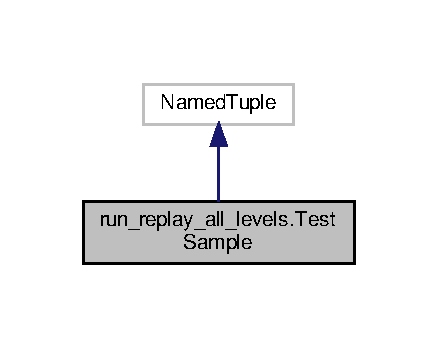
\includegraphics[width=210pt]{classrun__replay__all__levels_1_1TestSample__inherit__graph}
\end{center}
\end{figure}


Collaboration diagram for run\+\_\+replay\+\_\+all\+\_\+levels.\+Test\+Sample\+:
\nopagebreak
\begin{figure}[H]
\begin{center}
\leavevmode
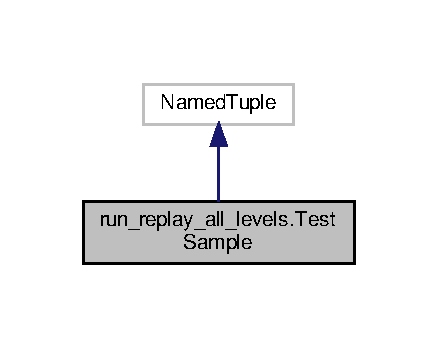
\includegraphics[width=210pt]{classrun__replay__all__levels_1_1TestSample__coll__graph}
\end{center}
\end{figure}


The documentation for this class was generated from the following file\+:\begin{DoxyCompactItemize}
\item 
scripts/run\+\_\+replay\+\_\+all\+\_\+levels.\+py\end{DoxyCompactItemize}

\hypertarget{classrun__evaluate__policy__all__levels_1_1TestSample}{}\section{run\+\_\+evaluate\+\_\+policy\+\_\+all\+\_\+levels.\+Test\+Sample Class Reference}
\label{classrun__evaluate__policy__all__levels_1_1TestSample}\index{run\+\_\+evaluate\+\_\+policy\+\_\+all\+\_\+levels.\+Test\+Sample@{run\+\_\+evaluate\+\_\+policy\+\_\+all\+\_\+levels.\+Test\+Sample}}


Inheritance diagram for run\+\_\+evaluate\+\_\+policy\+\_\+all\+\_\+levels.\+Test\+Sample\+:
\nopagebreak
\begin{figure}[H]
\begin{center}
\leavevmode
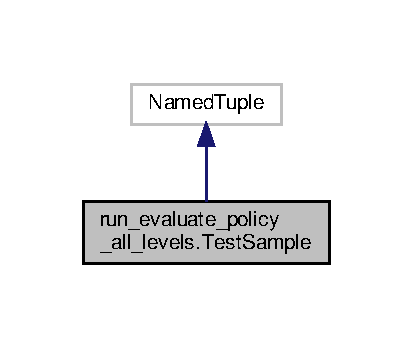
\includegraphics[width=198pt]{classrun__evaluate__policy__all__levels_1_1TestSample__inherit__graph}
\end{center}
\end{figure}


Collaboration diagram for run\+\_\+evaluate\+\_\+policy\+\_\+all\+\_\+levels.\+Test\+Sample\+:
\nopagebreak
\begin{figure}[H]
\begin{center}
\leavevmode
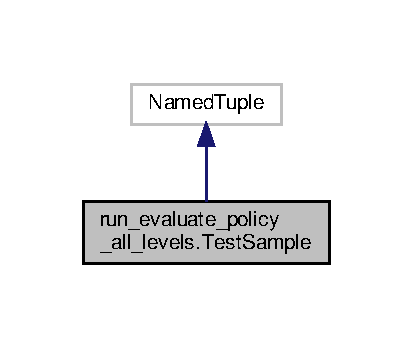
\includegraphics[width=198pt]{classrun__evaluate__policy__all__levels_1_1TestSample__coll__graph}
\end{center}
\end{figure}


The documentation for this class was generated from the following file\+:\begin{DoxyCompactItemize}
\item 
scripts/run\+\_\+evaluate\+\_\+policy\+\_\+all\+\_\+levels.\+py\end{DoxyCompactItemize}

\hypertarget{classtrifinger__simulation_1_1trifinger__platform_1_1TriCameraObservation}{}\section{trifinger\+\_\+simulation.\+trifinger\+\_\+platform.\+Tri\+Camera\+Observation Class Reference}
\label{classtrifinger__simulation_1_1trifinger__platform_1_1TriCameraObservation}\index{trifinger\+\_\+simulation.\+trifinger\+\_\+platform.\+Tri\+Camera\+Observation@{trifinger\+\_\+simulation.\+trifinger\+\_\+platform.\+Tri\+Camera\+Observation}}


Pure-\/python copy of trifinger\+\_\+cameras.\+tricamera.\+Tri\+Camera\+Observation.  


\subsection*{Public Member Functions}
\begin{DoxyCompactItemize}
\item 
\mbox{\Hypertarget{classtrifinger__simulation_1_1trifinger__platform_1_1TriCameraObservation_ab4dabbece119b22a5c939496a4e3e32e}\label{classtrifinger__simulation_1_1trifinger__platform_1_1TriCameraObservation_ab4dabbece119b22a5c939496a4e3e32e}} 
def {\bfseries \+\_\+\+\_\+init\+\_\+\+\_\+} (self)
\end{DoxyCompactItemize}
\subsection*{Public Attributes}
\begin{DoxyCompactItemize}
\item 
\mbox{\Hypertarget{classtrifinger__simulation_1_1trifinger__platform_1_1TriCameraObservation_a9e2b5fe60329e4affb7756934dd30b67}\label{classtrifinger__simulation_1_1trifinger__platform_1_1TriCameraObservation_a9e2b5fe60329e4affb7756934dd30b67}} 
{\bfseries cameras}
\end{DoxyCompactItemize}
\subsection*{Static Private Attributes}
\begin{DoxyCompactItemize}
\item 
\mbox{\Hypertarget{classtrifinger__simulation_1_1trifinger__platform_1_1TriCameraObservation_a6e2ca238101d10184a6945751db055b2}\label{classtrifinger__simulation_1_1trifinger__platform_1_1TriCameraObservation_a6e2ca238101d10184a6945751db055b2}} 
list {\bfseries \+\_\+\+\_\+slots\+\_\+\+\_\+} = \mbox{[}\char`\"{}cameras\char`\"{}\mbox{]}
\end{DoxyCompactItemize}


\subsection{Detailed Description}
Pure-\/python copy of trifinger\+\_\+cameras.\+tricamera.\+Tri\+Camera\+Observation. 



The documentation for this class was generated from the following file\+:\begin{DoxyCompactItemize}
\item 
python/trifinger\+\_\+simulation/trifinger\+\_\+platform.\+py\end{DoxyCompactItemize}

\hypertarget{classtrifinger__simulation_1_1camera_1_1TriFingerCameras}{}\section{trifinger\+\_\+simulation.\+camera.\+Tri\+Finger\+Cameras Class Reference}
\label{classtrifinger__simulation_1_1camera_1_1TriFingerCameras}\index{trifinger\+\_\+simulation.\+camera.\+Tri\+Finger\+Cameras@{trifinger\+\_\+simulation.\+camera.\+Tri\+Finger\+Cameras}}


Simulate the three cameras of the Tri\+Finger platform.  


\subsection*{Public Member Functions}
\begin{DoxyCompactItemize}
\item 
\mbox{\Hypertarget{classtrifinger__simulation_1_1camera_1_1TriFingerCameras_a9a72d28e90618b812d207115e04f7bc1}\label{classtrifinger__simulation_1_1camera_1_1TriFingerCameras_a9a72d28e90618b812d207115e04f7bc1}} 
def {\bfseries \+\_\+\+\_\+init\+\_\+\+\_\+} (self)
\item 
def \hyperlink{classtrifinger__simulation_1_1camera_1_1TriFingerCameras_ab87b4d284e9a42deebe874ad5fb233b9}{get\+\_\+images} (self)
\begin{DoxyCompactList}\small\item\em Get images. \end{DoxyCompactList}\end{DoxyCompactItemize}
\subsection*{Public Attributes}
\begin{DoxyCompactItemize}
\item 
\mbox{\Hypertarget{classtrifinger__simulation_1_1camera_1_1TriFingerCameras_a41e19e51c303a91ecc953c2b41c787b6}\label{classtrifinger__simulation_1_1camera_1_1TriFingerCameras_a41e19e51c303a91ecc953c2b41c787b6}} 
{\bfseries cameras}
\end{DoxyCompactItemize}


\subsection{Detailed Description}
Simulate the three cameras of the Tri\+Finger platform. 



\subsection{Member Function Documentation}
\mbox{\Hypertarget{classtrifinger__simulation_1_1camera_1_1TriFingerCameras_ab87b4d284e9a42deebe874ad5fb233b9}\label{classtrifinger__simulation_1_1camera_1_1TriFingerCameras_ab87b4d284e9a42deebe874ad5fb233b9}} 
\index{trifinger\+\_\+simulation\+::camera\+::\+Tri\+Finger\+Cameras@{trifinger\+\_\+simulation\+::camera\+::\+Tri\+Finger\+Cameras}!get\+\_\+images@{get\+\_\+images}}
\index{get\+\_\+images@{get\+\_\+images}!trifinger\+\_\+simulation\+::camera\+::\+Tri\+Finger\+Cameras@{trifinger\+\_\+simulation\+::camera\+::\+Tri\+Finger\+Cameras}}
\subsubsection{\texorpdfstring{get\+\_\+images()}{get\_images()}}
{\footnotesize\ttfamily def trifinger\+\_\+simulation.\+camera.\+Tri\+Finger\+Cameras.\+get\+\_\+images (\begin{DoxyParamCaption}\item[{}]{self }\end{DoxyParamCaption})}



Get images. 

\begin{DoxyReturn}{Returns}
List of images, one per camera. Order is \mbox{[}camera60, camera180, camera300\mbox{]}. See \hyperlink{classtrifinger__simulation_1_1camera_1_1Camera_a6055089009e1f63df5ced179e5c56254}{Camera.\+get\+\_\+image()} for details. 
\end{DoxyReturn}


The documentation for this class was generated from the following file\+:\begin{DoxyCompactItemize}
\item 
python/trifinger\+\_\+simulation/camera.\+py\end{DoxyCompactItemize}

\hypertarget{classtrifinger__simulation_1_1trifinger__platform_1_1TriFingerPlatform}{}\section{trifinger\+\_\+simulation.\+trifinger\+\_\+platform.\+Tri\+Finger\+Platform Class Reference}
\label{classtrifinger__simulation_1_1trifinger__platform_1_1TriFingerPlatform}\index{trifinger\+\_\+simulation.\+trifinger\+\_\+platform.\+Tri\+Finger\+Platform@{trifinger\+\_\+simulation.\+trifinger\+\_\+platform.\+Tri\+Finger\+Platform}}
\subsection*{Public Member Functions}
\begin{DoxyCompactItemize}
\item 
def \hyperlink{classtrifinger__simulation_1_1trifinger__platform_1_1TriFingerPlatform_a7005f891e60191ac633dc676129235d3}{\+\_\+\+\_\+init\+\_\+\+\_\+} (self, visualization=False, initial\+\_\+robot\+\_\+position=None, initial\+\_\+object\+\_\+pose=None, enable\+\_\+cameras=False)
\begin{DoxyCompactList}\small\item\em Initialize. \end{DoxyCompactList}\item 
def \hyperlink{classtrifinger__simulation_1_1trifinger__platform_1_1TriFingerPlatform_ada1b2f4cbf62c8fe0cd36617b0935786}{get\+\_\+time\+\_\+step} (self)
\begin{DoxyCompactList}\small\item\em Get simulation time step in seconds. \end{DoxyCompactList}\item 
\mbox{\Hypertarget{classtrifinger__simulation_1_1trifinger__platform_1_1TriFingerPlatform_aa0fc01b9ecadb2b3e740ca1d3feedc1a}\label{classtrifinger__simulation_1_1trifinger__platform_1_1TriFingerPlatform_aa0fc01b9ecadb2b3e740ca1d3feedc1a}} 
def {\bfseries append\+\_\+desired\+\_\+action} (self, action)
\item 
def \hyperlink{classtrifinger__simulation_1_1trifinger__platform_1_1TriFingerPlatform_ad46ed81c3e6c557c9cce2ce919b6110b}{get\+\_\+object\+\_\+pose} (self, t)
\begin{DoxyCompactList}\small\item\em Get object pose at time step t. \end{DoxyCompactList}\item 
def \hyperlink{classtrifinger__simulation_1_1trifinger__platform_1_1TriFingerPlatform_a805e6e931f01283be195d04a7138a3f4}{get\+\_\+camera\+\_\+observation} (self, t)
\begin{DoxyCompactList}\small\item\em Get camera observation at time step t. \end{DoxyCompactList}\item 
def \hyperlink{classtrifinger__simulation_1_1trifinger__platform_1_1TriFingerPlatform_a2f504c8f4c9681359440a0a33d25c0f4}{store\+\_\+action\+\_\+log} (self, filename)
\begin{DoxyCompactList}\small\item\em Store the action log to a J\+S\+ON file. \end{DoxyCompactList}\end{DoxyCompactItemize}
\subsection*{Public Attributes}
\begin{DoxyCompactItemize}
\item 
\mbox{\Hypertarget{classtrifinger__simulation_1_1trifinger__platform_1_1TriFingerPlatform_aa99761840d54c8b50d02f11267d15848}\label{classtrifinger__simulation_1_1trifinger__platform_1_1TriFingerPlatform_aa99761840d54c8b50d02f11267d15848}} 
{\bfseries enable\+\_\+cameras}
\item 
\mbox{\Hypertarget{classtrifinger__simulation_1_1trifinger__platform_1_1TriFingerPlatform_a9df538fe516621fb84a4b4aa4497961b}\label{classtrifinger__simulation_1_1trifinger__platform_1_1TriFingerPlatform_a9df538fe516621fb84a4b4aa4497961b}} 
{\bfseries simfinger}
\item 
\mbox{\Hypertarget{classtrifinger__simulation_1_1trifinger__platform_1_1TriFingerPlatform_a187854c0a1c9815d03c2796e868da03e}\label{classtrifinger__simulation_1_1trifinger__platform_1_1TriFingerPlatform_a187854c0a1c9815d03c2796e868da03e}} 
{\bfseries cube}
\item 
\mbox{\Hypertarget{classtrifinger__simulation_1_1trifinger__platform_1_1TriFingerPlatform_ab7b570c1996ad9e71582ced8af419bde}\label{classtrifinger__simulation_1_1trifinger__platform_1_1TriFingerPlatform_ab7b570c1996ad9e71582ced8af419bde}} 
{\bfseries tricamera}
\item 
\mbox{\Hypertarget{classtrifinger__simulation_1_1trifinger__platform_1_1TriFingerPlatform_ac1a05e90774daeeff64b31d89001c6f6}\label{classtrifinger__simulation_1_1trifinger__platform_1_1TriFingerPlatform_ac1a05e90774daeeff64b31d89001c6f6}} 
{\bfseries Action}
\item 
\mbox{\Hypertarget{classtrifinger__simulation_1_1trifinger__platform_1_1TriFingerPlatform_afa16f3b4d38d860c917fd7b96bd7549c}\label{classtrifinger__simulation_1_1trifinger__platform_1_1TriFingerPlatform_afa16f3b4d38d860c917fd7b96bd7549c}} 
{\bfseries get\+\_\+desired\+\_\+action}
\item 
\mbox{\Hypertarget{classtrifinger__simulation_1_1trifinger__platform_1_1TriFingerPlatform_af73b1f73050b144b6e8ad7d8ec427fa7}\label{classtrifinger__simulation_1_1trifinger__platform_1_1TriFingerPlatform_af73b1f73050b144b6e8ad7d8ec427fa7}} 
{\bfseries get\+\_\+applied\+\_\+action}
\item 
\mbox{\Hypertarget{classtrifinger__simulation_1_1trifinger__platform_1_1TriFingerPlatform_a8c354b04968190c1b76594adff7520cb}\label{classtrifinger__simulation_1_1trifinger__platform_1_1TriFingerPlatform_a8c354b04968190c1b76594adff7520cb}} 
{\bfseries get\+\_\+timestamp\+\_\+ms}
\item 
\mbox{\Hypertarget{classtrifinger__simulation_1_1trifinger__platform_1_1TriFingerPlatform_aef87c0a8eadbbef16dfb5383042ddaa7}\label{classtrifinger__simulation_1_1trifinger__platform_1_1TriFingerPlatform_aef87c0a8eadbbef16dfb5383042ddaa7}} 
{\bfseries get\+\_\+current\+\_\+timeindex}
\item 
\mbox{\Hypertarget{classtrifinger__simulation_1_1trifinger__platform_1_1TriFingerPlatform_a7740172e1dec9f4f96eb897b7f43236f}\label{classtrifinger__simulation_1_1trifinger__platform_1_1TriFingerPlatform_a7740172e1dec9f4f96eb897b7f43236f}} 
{\bfseries get\+\_\+robot\+\_\+observation}
\item 
\mbox{\Hypertarget{classtrifinger__simulation_1_1trifinger__platform_1_1TriFingerPlatform_a7b936de6a534c18ec7f357a7cd6a8483}\label{classtrifinger__simulation_1_1trifinger__platform_1_1TriFingerPlatform_a7b936de6a534c18ec7f357a7cd6a8483}} 
{\bfseries forward\+\_\+kinematics}
\end{DoxyCompactItemize}
\subsection*{Static Public Attributes}
\begin{DoxyCompactItemize}
\item 
\mbox{\Hypertarget{classtrifinger__simulation_1_1trifinger__platform_1_1TriFingerPlatform_a1bcbcb3250e4de77720249e70c69aaec}\label{classtrifinger__simulation_1_1trifinger__platform_1_1TriFingerPlatform_a1bcbcb3250e4de77720249e70c69aaec}} 
{\bfseries spaces} = Simple\+Namespace()
\item 
\mbox{\Hypertarget{classtrifinger__simulation_1_1trifinger__platform_1_1TriFingerPlatform_a03797f7e0c9faa00ee1912fd61ad2c5f}\label{classtrifinger__simulation_1_1trifinger__platform_1_1TriFingerPlatform_a03797f7e0c9faa00ee1912fd61ad2c5f}} 
{\bfseries robot\+\_\+torque}
\item 
\mbox{\Hypertarget{classtrifinger__simulation_1_1trifinger__platform_1_1TriFingerPlatform_a3a257b64352b25653947c9c5754deebd}\label{classtrifinger__simulation_1_1trifinger__platform_1_1TriFingerPlatform_a3a257b64352b25653947c9c5754deebd}} 
{\bfseries low}
\item 
\mbox{\Hypertarget{classtrifinger__simulation_1_1trifinger__platform_1_1TriFingerPlatform_a10785bc86490919e7596ed49394c2b08}\label{classtrifinger__simulation_1_1trifinger__platform_1_1TriFingerPlatform_a10785bc86490919e7596ed49394c2b08}} 
{\bfseries high}
\item 
\mbox{\Hypertarget{classtrifinger__simulation_1_1trifinger__platform_1_1TriFingerPlatform_ab50bdd7002eb9220d21b51ad080f0d11}\label{classtrifinger__simulation_1_1trifinger__platform_1_1TriFingerPlatform_ab50bdd7002eb9220d21b51ad080f0d11}} 
{\bfseries default}
\item 
\mbox{\Hypertarget{classtrifinger__simulation_1_1trifinger__platform_1_1TriFingerPlatform_a527559d524506159887973e11f18e143}\label{classtrifinger__simulation_1_1trifinger__platform_1_1TriFingerPlatform_a527559d524506159887973e11f18e143}} 
{\bfseries robot\+\_\+position}
\item 
\mbox{\Hypertarget{classtrifinger__simulation_1_1trifinger__platform_1_1TriFingerPlatform_ac047cdcdd92c0184ad6ce57a35aa2e60}\label{classtrifinger__simulation_1_1trifinger__platform_1_1TriFingerPlatform_ac047cdcdd92c0184ad6ce57a35aa2e60}} 
{\bfseries robot\+\_\+velocity}
\item 
\mbox{\Hypertarget{classtrifinger__simulation_1_1trifinger__platform_1_1TriFingerPlatform_a8b751f2d5314bd5db9e314285b9e08b6}\label{classtrifinger__simulation_1_1trifinger__platform_1_1TriFingerPlatform_a8b751f2d5314bd5db9e314285b9e08b6}} 
{\bfseries object\+\_\+position}
\item 
\mbox{\Hypertarget{classtrifinger__simulation_1_1trifinger__platform_1_1TriFingerPlatform_ab2187a510141b0e79671cc860c6031b7}\label{classtrifinger__simulation_1_1trifinger__platform_1_1TriFingerPlatform_ab2187a510141b0e79671cc860c6031b7}} 
{\bfseries object\+\_\+orientation}
\item 
\mbox{\Hypertarget{classtrifinger__simulation_1_1trifinger__platform_1_1TriFingerPlatform_a752fe7f768964427e2b67f07c2cbcfe2}\label{classtrifinger__simulation_1_1trifinger__platform_1_1TriFingerPlatform_a752fe7f768964427e2b67f07c2cbcfe2}} 
{\bfseries gym}
\end{DoxyCompactItemize}
\subsection*{Private Member Functions}
\begin{DoxyCompactItemize}
\item 
\mbox{\Hypertarget{classtrifinger__simulation_1_1trifinger__platform_1_1TriFingerPlatform_aeb8f1699a36b339da4a787308c3f3731}\label{classtrifinger__simulation_1_1trifinger__platform_1_1TriFingerPlatform_aeb8f1699a36b339da4a787308c3f3731}} 
def {\bfseries \+\_\+compute\+\_\+camera\+\_\+update\+\_\+step\+\_\+interval} (self)
\item 
\mbox{\Hypertarget{classtrifinger__simulation_1_1trifinger__platform_1_1TriFingerPlatform_a5ed284dedee9899105e5fc68e9c958a0}\label{classtrifinger__simulation_1_1trifinger__platform_1_1TriFingerPlatform_a5ed284dedee9899105e5fc68e9c958a0}} 
def {\bfseries \+\_\+get\+\_\+current\+\_\+object\+\_\+pose} (self, t=None)
\item 
\mbox{\Hypertarget{classtrifinger__simulation_1_1trifinger__platform_1_1TriFingerPlatform_a185d07d66efca2fc4f42d1717da1dc0c}\label{classtrifinger__simulation_1_1trifinger__platform_1_1TriFingerPlatform_a185d07d66efca2fc4f42d1717da1dc0c}} 
def {\bfseries \+\_\+get\+\_\+current\+\_\+camera\+\_\+observation} (self, t=None)
\end{DoxyCompactItemize}
\subsection*{Private Attributes}
\begin{DoxyCompactItemize}
\item 
\mbox{\Hypertarget{classtrifinger__simulation_1_1trifinger__platform_1_1TriFingerPlatform_ad5193694ebd2d75034ea7e735be79c73}\label{classtrifinger__simulation_1_1trifinger__platform_1_1TriFingerPlatform_ad5193694ebd2d75034ea7e735be79c73}} 
{\bfseries \+\_\+camera\+\_\+rate\+\_\+fps}
\item 
\mbox{\Hypertarget{classtrifinger__simulation_1_1trifinger__platform_1_1TriFingerPlatform_adcbc32c8b3776632e2e8ab6274315ca4}\label{classtrifinger__simulation_1_1trifinger__platform_1_1TriFingerPlatform_adcbc32c8b3776632e2e8ab6274315ca4}} 
{\bfseries \+\_\+time\+\_\+step}
\item 
\mbox{\Hypertarget{classtrifinger__simulation_1_1trifinger__platform_1_1TriFingerPlatform_a4de25e81797ba3da9ff9222d20b98572}\label{classtrifinger__simulation_1_1trifinger__platform_1_1TriFingerPlatform_a4de25e81797ba3da9ff9222d20b98572}} 
{\bfseries \+\_\+next\+\_\+camera\+\_\+update\+\_\+step}
\item 
\mbox{\Hypertarget{classtrifinger__simulation_1_1trifinger__platform_1_1TriFingerPlatform_afd410762f126abcc6d0559cced42128b}\label{classtrifinger__simulation_1_1trifinger__platform_1_1TriFingerPlatform_afd410762f126abcc6d0559cced42128b}} 
{\bfseries \+\_\+action\+\_\+log}
\item 
\mbox{\Hypertarget{classtrifinger__simulation_1_1trifinger__platform_1_1TriFingerPlatform_a9446da8fdf18a63fe457212f556fcf32}\label{classtrifinger__simulation_1_1trifinger__platform_1_1TriFingerPlatform_a9446da8fdf18a63fe457212f556fcf32}} 
{\bfseries \+\_\+object\+\_\+pose\+\_\+t}
\item 
\mbox{\Hypertarget{classtrifinger__simulation_1_1trifinger__platform_1_1TriFingerPlatform_a8afba4b7b79d816d74e7bef07202ff48}\label{classtrifinger__simulation_1_1trifinger__platform_1_1TriFingerPlatform_a8afba4b7b79d816d74e7bef07202ff48}} 
{\bfseries \+\_\+camera\+\_\+observation\+\_\+t}
\end{DoxyCompactItemize}
\subsection*{Static Private Attributes}
\begin{DoxyCompactItemize}
\item 
\mbox{\Hypertarget{classtrifinger__simulation_1_1trifinger__platform_1_1TriFingerPlatform_a155ceed878068737f4f88d8dd1893a5b}\label{classtrifinger__simulation_1_1trifinger__platform_1_1TriFingerPlatform_a155ceed878068737f4f88d8dd1893a5b}} 
int {\bfseries \+\_\+n\+\_\+joints}
\item 
\mbox{\Hypertarget{classtrifinger__simulation_1_1trifinger__platform_1_1TriFingerPlatform_a261d426c680071f7c75bcf32470bcdbf}\label{classtrifinger__simulation_1_1trifinger__platform_1_1TriFingerPlatform_a261d426c680071f7c75bcf32470bcdbf}} 
int {\bfseries \+\_\+n\+\_\+fingers}
\item 
\mbox{\Hypertarget{classtrifinger__simulation_1_1trifinger__platform_1_1TriFingerPlatform_aaeb7ecab6a48a5165b9598874b59ee8b}\label{classtrifinger__simulation_1_1trifinger__platform_1_1TriFingerPlatform_aaeb7ecab6a48a5165b9598874b59ee8b}} 
float {\bfseries \+\_\+max\+\_\+torque\+\_\+\+Nm}
\item 
\mbox{\Hypertarget{classtrifinger__simulation_1_1trifinger__platform_1_1TriFingerPlatform_a50e345039aa1be52a8f776a58dfad75d}\label{classtrifinger__simulation_1_1trifinger__platform_1_1TriFingerPlatform_a50e345039aa1be52a8f776a58dfad75d}} 
int {\bfseries \+\_\+max\+\_\+velocity\+\_\+radps}
\end{DoxyCompactItemize}


\subsection{Constructor \& Destructor Documentation}
\mbox{\Hypertarget{classtrifinger__simulation_1_1trifinger__platform_1_1TriFingerPlatform_a7005f891e60191ac633dc676129235d3}\label{classtrifinger__simulation_1_1trifinger__platform_1_1TriFingerPlatform_a7005f891e60191ac633dc676129235d3}} 
\index{trifinger\+\_\+simulation\+::trifinger\+\_\+platform\+::\+Tri\+Finger\+Platform@{trifinger\+\_\+simulation\+::trifinger\+\_\+platform\+::\+Tri\+Finger\+Platform}!\+\_\+\+\_\+init\+\_\+\+\_\+@{\+\_\+\+\_\+init\+\_\+\+\_\+}}
\index{\+\_\+\+\_\+init\+\_\+\+\_\+@{\+\_\+\+\_\+init\+\_\+\+\_\+}!trifinger\+\_\+simulation\+::trifinger\+\_\+platform\+::\+Tri\+Finger\+Platform@{trifinger\+\_\+simulation\+::trifinger\+\_\+platform\+::\+Tri\+Finger\+Platform}}
\subsubsection{\texorpdfstring{\+\_\+\+\_\+init\+\_\+\+\_\+()}{\_\_init\_\_()}}
{\footnotesize\ttfamily def trifinger\+\_\+simulation.\+trifinger\+\_\+platform.\+Tri\+Finger\+Platform.\+\_\+\+\_\+init\+\_\+\+\_\+ (\begin{DoxyParamCaption}\item[{}]{self,  }\item[{}]{visualization = {\ttfamily False},  }\item[{}]{initial\+\_\+robot\+\_\+position = {\ttfamily None},  }\item[{}]{initial\+\_\+object\+\_\+pose = {\ttfamily None},  }\item[{}]{enable\+\_\+cameras = {\ttfamily False} }\end{DoxyParamCaption})}



Initialize. 


\begin{DoxyParams}{Parameters}
{\em visualization} & Set to true to run visualization. \\
\hline
{\em initial\+\_\+robot\+\_\+position} & Initial robot joint angles \\
\hline
{\em initial\+\_\+object\+\_\+pose} & Initial pose for the manipulation object. Can be any object with attributes {\ttfamily position} (x, y, z) and {\ttfamily orientation} (x, y, z, w). This is optional, if not set, a random pose will be sampled. \\
\hline
{\em enable\+\_\+cameras} & Set to true to enable camera observations. By default this is disabled as rendering of images takes a lot of computational power. Therefore the cameras should only be enabled if the images are actually used. \\
\hline
\end{DoxyParams}


\subsection{Member Function Documentation}
\mbox{\Hypertarget{classtrifinger__simulation_1_1trifinger__platform_1_1TriFingerPlatform_a805e6e931f01283be195d04a7138a3f4}\label{classtrifinger__simulation_1_1trifinger__platform_1_1TriFingerPlatform_a805e6e931f01283be195d04a7138a3f4}} 
\index{trifinger\+\_\+simulation\+::trifinger\+\_\+platform\+::\+Tri\+Finger\+Platform@{trifinger\+\_\+simulation\+::trifinger\+\_\+platform\+::\+Tri\+Finger\+Platform}!get\+\_\+camera\+\_\+observation@{get\+\_\+camera\+\_\+observation}}
\index{get\+\_\+camera\+\_\+observation@{get\+\_\+camera\+\_\+observation}!trifinger\+\_\+simulation\+::trifinger\+\_\+platform\+::\+Tri\+Finger\+Platform@{trifinger\+\_\+simulation\+::trifinger\+\_\+platform\+::\+Tri\+Finger\+Platform}}
\subsubsection{\texorpdfstring{get\+\_\+camera\+\_\+observation()}{get\_camera\_observation()}}
{\footnotesize\ttfamily def trifinger\+\_\+simulation.\+trifinger\+\_\+platform.\+Tri\+Finger\+Platform.\+get\+\_\+camera\+\_\+observation (\begin{DoxyParamCaption}\item[{}]{self,  }\item[{}]{t }\end{DoxyParamCaption})}



Get camera observation at time step t. 


\begin{DoxyParams}{Parameters}
{\em t} & The time index of the step for which the observation is requested. Only the value returned by the last call of \+:meth\+:{\ttfamily $\sim$append\+\_\+desired\+\_\+action} is valid.\\
\hline
\end{DoxyParams}
\begin{DoxyReturn}{Returns}


\hyperlink{classtrifinger__simulation_1_1trifinger__platform_1_1TriCameraObservation}{Tri\+Camera\+Observation} Observations of the three cameras. Images are rendered in the simulation. Note that they are not optimized to look realistically.
\end{DoxyReturn}

\begin{DoxyExceptions}{Exceptions}
{\em Value\+Error} & If invalid time index {\ttfamily t} is passed. \\
\hline
\end{DoxyExceptions}
\mbox{\Hypertarget{classtrifinger__simulation_1_1trifinger__platform_1_1TriFingerPlatform_ad46ed81c3e6c557c9cce2ce919b6110b}\label{classtrifinger__simulation_1_1trifinger__platform_1_1TriFingerPlatform_ad46ed81c3e6c557c9cce2ce919b6110b}} 
\index{trifinger\+\_\+simulation\+::trifinger\+\_\+platform\+::\+Tri\+Finger\+Platform@{trifinger\+\_\+simulation\+::trifinger\+\_\+platform\+::\+Tri\+Finger\+Platform}!get\+\_\+object\+\_\+pose@{get\+\_\+object\+\_\+pose}}
\index{get\+\_\+object\+\_\+pose@{get\+\_\+object\+\_\+pose}!trifinger\+\_\+simulation\+::trifinger\+\_\+platform\+::\+Tri\+Finger\+Platform@{trifinger\+\_\+simulation\+::trifinger\+\_\+platform\+::\+Tri\+Finger\+Platform}}
\subsubsection{\texorpdfstring{get\+\_\+object\+\_\+pose()}{get\_object\_pose()}}
{\footnotesize\ttfamily def trifinger\+\_\+simulation.\+trifinger\+\_\+platform.\+Tri\+Finger\+Platform.\+get\+\_\+object\+\_\+pose (\begin{DoxyParamCaption}\item[{}]{self,  }\item[{}]{t }\end{DoxyParamCaption})}



Get object pose at time step t. 


\begin{DoxyParams}{Parameters}
{\em t} & The time index of the step for which the object pose is requested. Only the value returned by the last call of \+:meth\+:{\ttfamily $\sim$append\+\_\+desired\+\_\+action} is valid.\\
\hline
\end{DoxyParams}
\begin{DoxyReturn}{Returns}


\hyperlink{classtrifinger__simulation_1_1trifinger__platform_1_1ObjectPose}{Object\+Pose} Pose of the object. Values come directly from the simulation without adding noise, so the confidence is 1.\+0.
\end{DoxyReturn}

\begin{DoxyExceptions}{Exceptions}
{\em Value\+Error} & If invalid time index {\ttfamily t} is passed. \\
\hline
\end{DoxyExceptions}
\mbox{\Hypertarget{classtrifinger__simulation_1_1trifinger__platform_1_1TriFingerPlatform_ada1b2f4cbf62c8fe0cd36617b0935786}\label{classtrifinger__simulation_1_1trifinger__platform_1_1TriFingerPlatform_ada1b2f4cbf62c8fe0cd36617b0935786}} 
\index{trifinger\+\_\+simulation\+::trifinger\+\_\+platform\+::\+Tri\+Finger\+Platform@{trifinger\+\_\+simulation\+::trifinger\+\_\+platform\+::\+Tri\+Finger\+Platform}!get\+\_\+time\+\_\+step@{get\+\_\+time\+\_\+step}}
\index{get\+\_\+time\+\_\+step@{get\+\_\+time\+\_\+step}!trifinger\+\_\+simulation\+::trifinger\+\_\+platform\+::\+Tri\+Finger\+Platform@{trifinger\+\_\+simulation\+::trifinger\+\_\+platform\+::\+Tri\+Finger\+Platform}}
\subsubsection{\texorpdfstring{get\+\_\+time\+\_\+step()}{get\_time\_step()}}
{\footnotesize\ttfamily def trifinger\+\_\+simulation.\+trifinger\+\_\+platform.\+Tri\+Finger\+Platform.\+get\+\_\+time\+\_\+step (\begin{DoxyParamCaption}\item[{}]{self }\end{DoxyParamCaption})}



Get simulation time step in seconds. 

\mbox{\Hypertarget{classtrifinger__simulation_1_1trifinger__platform_1_1TriFingerPlatform_a2f504c8f4c9681359440a0a33d25c0f4}\label{classtrifinger__simulation_1_1trifinger__platform_1_1TriFingerPlatform_a2f504c8f4c9681359440a0a33d25c0f4}} 
\index{trifinger\+\_\+simulation\+::trifinger\+\_\+platform\+::\+Tri\+Finger\+Platform@{trifinger\+\_\+simulation\+::trifinger\+\_\+platform\+::\+Tri\+Finger\+Platform}!store\+\_\+action\+\_\+log@{store\+\_\+action\+\_\+log}}
\index{store\+\_\+action\+\_\+log@{store\+\_\+action\+\_\+log}!trifinger\+\_\+simulation\+::trifinger\+\_\+platform\+::\+Tri\+Finger\+Platform@{trifinger\+\_\+simulation\+::trifinger\+\_\+platform\+::\+Tri\+Finger\+Platform}}
\subsubsection{\texorpdfstring{store\+\_\+action\+\_\+log()}{store\_action\_log()}}
{\footnotesize\ttfamily def trifinger\+\_\+simulation.\+trifinger\+\_\+platform.\+Tri\+Finger\+Platform.\+store\+\_\+action\+\_\+log (\begin{DoxyParamCaption}\item[{}]{self,  }\item[{}]{filename }\end{DoxyParamCaption})}



Store the action log to a J\+S\+ON file. 


\begin{DoxyParams}{Parameters}
{\em filename} & Path to the J\+S\+ON file to which the log shall be written. If the file exists already, it will be overwritten. \\
\hline
\end{DoxyParams}


The documentation for this class was generated from the following file\+:\begin{DoxyCompactItemize}
\item 
python/trifinger\+\_\+simulation/trifinger\+\_\+platform.\+py\end{DoxyCompactItemize}

\hypertarget{classtrifinger__simulation_1_1gym__wrapper_1_1envs_1_1trifinger__push_1_1TriFingerPush}{}\section{trifinger\+\_\+simulation.\+gym\+\_\+wrapper.\+envs.\+trifinger\+\_\+push.\+Tri\+Finger\+Push Class Reference}
\label{classtrifinger__simulation_1_1gym__wrapper_1_1envs_1_1trifinger__push_1_1TriFingerPush}\index{trifinger\+\_\+simulation.\+gym\+\_\+wrapper.\+envs.\+trifinger\+\_\+push.\+Tri\+Finger\+Push@{trifinger\+\_\+simulation.\+gym\+\_\+wrapper.\+envs.\+trifinger\+\_\+push.\+Tri\+Finger\+Push}}


A gym environment to enable training on any of the valid robots, real or simulated, for the task of pushing.  




Inheritance diagram for trifinger\+\_\+simulation.\+gym\+\_\+wrapper.\+envs.\+trifinger\+\_\+push.\+Tri\+Finger\+Push\+:
\nopagebreak
\begin{figure}[H]
\begin{center}
\leavevmode
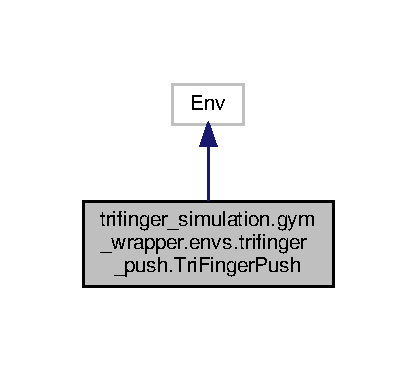
\includegraphics[width=200pt]{classtrifinger__simulation_1_1gym__wrapper_1_1envs_1_1trifinger__push_1_1TriFingerPush__inherit__graph}
\end{center}
\end{figure}


Collaboration diagram for trifinger\+\_\+simulation.\+gym\+\_\+wrapper.\+envs.\+trifinger\+\_\+push.\+Tri\+Finger\+Push\+:
\nopagebreak
\begin{figure}[H]
\begin{center}
\leavevmode
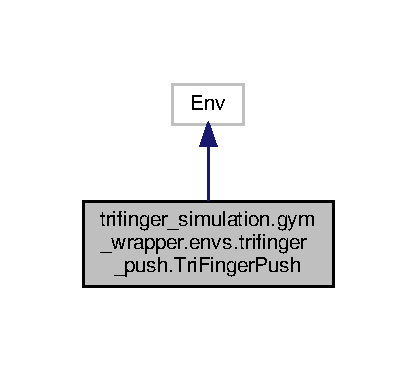
\includegraphics[width=200pt]{classtrifinger__simulation_1_1gym__wrapper_1_1envs_1_1trifinger__push_1_1TriFingerPush__coll__graph}
\end{center}
\end{figure}
\subsection*{Public Member Functions}
\begin{DoxyCompactItemize}
\item 
def \hyperlink{classtrifinger__simulation_1_1gym__wrapper_1_1envs_1_1trifinger__push_1_1TriFingerPush_aa6c84179b96f31cd9c464598c14cee39}{\+\_\+\+\_\+init\+\_\+\+\_\+} (self, control\+\_\+rate\+\_\+s, finger\+\_\+type, enable\+\_\+visualization)
\begin{DoxyCompactList}\small\item\em Intializes the constituents of the pushing environment. \end{DoxyCompactList}\item 
def \hyperlink{classtrifinger__simulation_1_1gym__wrapper_1_1envs_1_1trifinger__push_1_1TriFingerPush_a9d02a422dd3e4fc843c1625bc3b48563}{step} (self, action)
\begin{DoxyCompactList}\small\item\em The env step method. \end{DoxyCompactList}\item 
def \hyperlink{classtrifinger__simulation_1_1gym__wrapper_1_1envs_1_1trifinger__push_1_1TriFingerPush_a37f86f66dd9d3268f0df751fc295df23}{reset} (self)
\begin{DoxyCompactList}\small\item\em Episode reset. \end{DoxyCompactList}\end{DoxyCompactItemize}
\subsection*{Public Attributes}
\begin{DoxyCompactItemize}
\item 
\mbox{\Hypertarget{classtrifinger__simulation_1_1gym__wrapper_1_1envs_1_1trifinger__push_1_1TriFingerPush_a56b76416d3aae829300b0c0ee4e976f8}\label{classtrifinger__simulation_1_1gym__wrapper_1_1envs_1_1trifinger__push_1_1TriFingerPush_a56b76416d3aae829300b0c0ee4e976f8}} 
{\bfseries finger}
\item 
\mbox{\Hypertarget{classtrifinger__simulation_1_1gym__wrapper_1_1envs_1_1trifinger__push_1_1TriFingerPush_a7261e05eeeeab9b7639c4727ef647c4c}\label{classtrifinger__simulation_1_1gym__wrapper_1_1envs_1_1trifinger__push_1_1TriFingerPush_a7261e05eeeeab9b7639c4727ef647c4c}} 
{\bfseries num\+\_\+fingers}
\item 
\mbox{\Hypertarget{classtrifinger__simulation_1_1gym__wrapper_1_1envs_1_1trifinger__push_1_1TriFingerPush_a3f2a2f104565c1dd941a4eb3ac5ae6d2}\label{classtrifinger__simulation_1_1gym__wrapper_1_1envs_1_1trifinger__push_1_1TriFingerPush_a3f2a2f104565c1dd941a4eb3ac5ae6d2}} 
{\bfseries steps\+\_\+per\+\_\+control}
\item 
\mbox{\Hypertarget{classtrifinger__simulation_1_1gym__wrapper_1_1envs_1_1trifinger__push_1_1TriFingerPush_ac44c94e757df84d9523d3a54daf629c8}\label{classtrifinger__simulation_1_1gym__wrapper_1_1envs_1_1trifinger__push_1_1TriFingerPush_ac44c94e757df84d9523d3a54daf629c8}} 
{\bfseries observations\+\_\+keys}
\item 
\mbox{\Hypertarget{classtrifinger__simulation_1_1gym__wrapper_1_1envs_1_1trifinger__push_1_1TriFingerPush_a599122295b3d9dd30064075097ea6c5d}\label{classtrifinger__simulation_1_1gym__wrapper_1_1envs_1_1trifinger__push_1_1TriFingerPush_a599122295b3d9dd30064075097ea6c5d}} 
{\bfseries observations\+\_\+sizes}
\item 
\mbox{\Hypertarget{classtrifinger__simulation_1_1gym__wrapper_1_1envs_1_1trifinger__push_1_1TriFingerPush_aa53c1114a0298a7994eae8efe64dc19f}\label{classtrifinger__simulation_1_1gym__wrapper_1_1envs_1_1trifinger__push_1_1TriFingerPush_aa53c1114a0298a7994eae8efe64dc19f}} 
{\bfseries spaces}
\item 
\mbox{\Hypertarget{classtrifinger__simulation_1_1gym__wrapper_1_1envs_1_1trifinger__push_1_1TriFingerPush_af3b2003b9f169fd2b8ec4370961ffe26}\label{classtrifinger__simulation_1_1gym__wrapper_1_1envs_1_1trifinger__push_1_1TriFingerPush_af3b2003b9f169fd2b8ec4370961ffe26}} 
{\bfseries unscaled\+\_\+observation\+\_\+space}
\item 
\mbox{\Hypertarget{classtrifinger__simulation_1_1gym__wrapper_1_1envs_1_1trifinger__push_1_1TriFingerPush_ae9807ed5917fb16b2eb5e7a2f168712a}\label{classtrifinger__simulation_1_1gym__wrapper_1_1envs_1_1trifinger__push_1_1TriFingerPush_ae9807ed5917fb16b2eb5e7a2f168712a}} 
{\bfseries unscaled\+\_\+action\+\_\+space}
\item 
\mbox{\Hypertarget{classtrifinger__simulation_1_1gym__wrapper_1_1envs_1_1trifinger__push_1_1TriFingerPush_a9ea94f92642ddfb4335690e1a3d0a27f}\label{classtrifinger__simulation_1_1gym__wrapper_1_1envs_1_1trifinger__push_1_1TriFingerPush_a9ea94f92642ddfb4335690e1a3d0a27f}} 
{\bfseries observation\+\_\+space}
\item 
\mbox{\Hypertarget{classtrifinger__simulation_1_1gym__wrapper_1_1envs_1_1trifinger__push_1_1TriFingerPush_aa6393fef17a17dc420e3aa7002c4cbc6}\label{classtrifinger__simulation_1_1gym__wrapper_1_1envs_1_1trifinger__push_1_1TriFingerPush_aa6393fef17a17dc420e3aa7002c4cbc6}} 
{\bfseries action\+\_\+space}
\item 
\mbox{\Hypertarget{classtrifinger__simulation_1_1gym__wrapper_1_1envs_1_1trifinger__push_1_1TriFingerPush_a2b2033880a6185b431025ff555665084}\label{classtrifinger__simulation_1_1gym__wrapper_1_1envs_1_1trifinger__push_1_1TriFingerPush_a2b2033880a6185b431025ff555665084}} 
{\bfseries logger}
\item 
\mbox{\Hypertarget{classtrifinger__simulation_1_1gym__wrapper_1_1envs_1_1trifinger__push_1_1TriFingerPush_a4dbf8da7c94b9b278d27f493f958b1a1}\label{classtrifinger__simulation_1_1gym__wrapper_1_1envs_1_1trifinger__push_1_1TriFingerPush_a4dbf8da7c94b9b278d27f493f958b1a1}} 
{\bfseries block}
\item 
\mbox{\Hypertarget{classtrifinger__simulation_1_1gym__wrapper_1_1envs_1_1trifinger__push_1_1TriFingerPush_ae956c9651e6bc2600379fde2d3e5becd}\label{classtrifinger__simulation_1_1gym__wrapper_1_1envs_1_1trifinger__push_1_1TriFingerPush_ae956c9651e6bc2600379fde2d3e5becd}} 
{\bfseries goal\+\_\+marker}
\item 
\mbox{\Hypertarget{classtrifinger__simulation_1_1gym__wrapper_1_1envs_1_1trifinger__push_1_1TriFingerPush_a8e0e6d9e2a6e704d03d56740ce775ac3}\label{classtrifinger__simulation_1_1gym__wrapper_1_1envs_1_1trifinger__push_1_1TriFingerPush_a8e0e6d9e2a6e704d03d56740ce775ac3}} 
{\bfseries goal}
\item 
\mbox{\Hypertarget{classtrifinger__simulation_1_1gym__wrapper_1_1envs_1_1trifinger__push_1_1TriFingerPush_af58e48366f404510bd8d295623fce01e}\label{classtrifinger__simulation_1_1gym__wrapper_1_1envs_1_1trifinger__push_1_1TriFingerPush_af58e48366f404510bd8d295623fce01e}} 
{\bfseries block\+\_\+position}
\end{DoxyCompactItemize}
\subsection*{Private Member Functions}
\begin{DoxyCompactItemize}
\item 
def \hyperlink{classtrifinger__simulation_1_1gym__wrapper_1_1envs_1_1trifinger__push_1_1TriFingerPush_a5dcce1db0f4090f057eaa420d13a58d2}{\+\_\+compute\+\_\+reward} (self, object\+\_\+position, goal)
\begin{DoxyCompactList}\small\item\em The reward function of the environment. \end{DoxyCompactList}\item 
def \hyperlink{classtrifinger__simulation_1_1gym__wrapper_1_1envs_1_1trifinger__push_1_1TriFingerPush_a1ca7fa96ffd63170bad1f341b734b388}{\+\_\+get\+\_\+state} (self, observation, action, log\+\_\+observation=False)
\begin{DoxyCompactList}\small\item\em Get the current observation from the env for the agent. \end{DoxyCompactList}\end{DoxyCompactItemize}


\subsection{Detailed Description}
A gym environment to enable training on any of the valid robots, real or simulated, for the task of pushing. 

\subsection{Constructor \& Destructor Documentation}
\mbox{\Hypertarget{classtrifinger__simulation_1_1gym__wrapper_1_1envs_1_1trifinger__push_1_1TriFingerPush_aa6c84179b96f31cd9c464598c14cee39}\label{classtrifinger__simulation_1_1gym__wrapper_1_1envs_1_1trifinger__push_1_1TriFingerPush_aa6c84179b96f31cd9c464598c14cee39}} 
\index{trifinger\+\_\+simulation\+::gym\+\_\+wrapper\+::envs\+::trifinger\+\_\+push\+::\+Tri\+Finger\+Push@{trifinger\+\_\+simulation\+::gym\+\_\+wrapper\+::envs\+::trifinger\+\_\+push\+::\+Tri\+Finger\+Push}!\+\_\+\+\_\+init\+\_\+\+\_\+@{\+\_\+\+\_\+init\+\_\+\+\_\+}}
\index{\+\_\+\+\_\+init\+\_\+\+\_\+@{\+\_\+\+\_\+init\+\_\+\+\_\+}!trifinger\+\_\+simulation\+::gym\+\_\+wrapper\+::envs\+::trifinger\+\_\+push\+::\+Tri\+Finger\+Push@{trifinger\+\_\+simulation\+::gym\+\_\+wrapper\+::envs\+::trifinger\+\_\+push\+::\+Tri\+Finger\+Push}}
\subsubsection{\texorpdfstring{\+\_\+\+\_\+init\+\_\+\+\_\+()}{\_\_init\_\_()}}
{\footnotesize\ttfamily def trifinger\+\_\+simulation.\+gym\+\_\+wrapper.\+envs.\+trifinger\+\_\+push.\+Tri\+Finger\+Push.\+\_\+\+\_\+init\+\_\+\+\_\+ (\begin{DoxyParamCaption}\item[{}]{self,  }\item[{}]{control\+\_\+rate\+\_\+s,  }\item[{}]{finger\+\_\+type,  }\item[{}]{enable\+\_\+visualization }\end{DoxyParamCaption})}



Intializes the constituents of the pushing environment. 

Constructor sets up the finger robot depending on the finger type, sets up the observation and action spaces, smoothing for reducing jitter on the robot, and provides for a way to synchronize robots being trained independently.


\begin{DoxyParams}{Parameters}
{\em control\+\_\+rate\+\_\+s} & the rate (in seconds) at which step method of the env will run. The actual robot controller may run at a higher rate, so this is used to compute the number of robot control updates per environment step. \\
\hline
{\em finger\+\_\+type} & Name of the finger type. In order to get a list of the valid finger types, call \+:meth\+:{\ttfamily .finger\+\_\+types\+\_\+data.\+get\+\_\+valid\+\_\+finger\+\_\+types} \\
\hline
{\em enable\+\_\+visualization} & if the simulation env is to be \\
\hline
{\em visualized} & \\
\hline
\end{DoxyParams}


\subsection{Member Function Documentation}
\mbox{\Hypertarget{classtrifinger__simulation_1_1gym__wrapper_1_1envs_1_1trifinger__push_1_1TriFingerPush_a5dcce1db0f4090f057eaa420d13a58d2}\label{classtrifinger__simulation_1_1gym__wrapper_1_1envs_1_1trifinger__push_1_1TriFingerPush_a5dcce1db0f4090f057eaa420d13a58d2}} 
\index{trifinger\+\_\+simulation\+::gym\+\_\+wrapper\+::envs\+::trifinger\+\_\+push\+::\+Tri\+Finger\+Push@{trifinger\+\_\+simulation\+::gym\+\_\+wrapper\+::envs\+::trifinger\+\_\+push\+::\+Tri\+Finger\+Push}!\+\_\+compute\+\_\+reward@{\+\_\+compute\+\_\+reward}}
\index{\+\_\+compute\+\_\+reward@{\+\_\+compute\+\_\+reward}!trifinger\+\_\+simulation\+::gym\+\_\+wrapper\+::envs\+::trifinger\+\_\+push\+::\+Tri\+Finger\+Push@{trifinger\+\_\+simulation\+::gym\+\_\+wrapper\+::envs\+::trifinger\+\_\+push\+::\+Tri\+Finger\+Push}}
\subsubsection{\texorpdfstring{\+\_\+compute\+\_\+reward()}{\_compute\_reward()}}
{\footnotesize\ttfamily def trifinger\+\_\+simulation.\+gym\+\_\+wrapper.\+envs.\+trifinger\+\_\+push.\+Tri\+Finger\+Push.\+\_\+compute\+\_\+reward (\begin{DoxyParamCaption}\item[{}]{self,  }\item[{}]{object\+\_\+position,  }\item[{}]{goal }\end{DoxyParamCaption})\hspace{0.3cm}{\ttfamily [private]}}



The reward function of the environment. 


\begin{DoxyParams}{Parameters}
{\em observation} & the observation at the current step \\
\hline
{\em goal} & the desired goal for the episode\\
\hline
\end{DoxyParams}
\begin{DoxyReturn}{Returns}
the reward, and the done signal 
\end{DoxyReturn}
\mbox{\Hypertarget{classtrifinger__simulation_1_1gym__wrapper_1_1envs_1_1trifinger__push_1_1TriFingerPush_a1ca7fa96ffd63170bad1f341b734b388}\label{classtrifinger__simulation_1_1gym__wrapper_1_1envs_1_1trifinger__push_1_1TriFingerPush_a1ca7fa96ffd63170bad1f341b734b388}} 
\index{trifinger\+\_\+simulation\+::gym\+\_\+wrapper\+::envs\+::trifinger\+\_\+push\+::\+Tri\+Finger\+Push@{trifinger\+\_\+simulation\+::gym\+\_\+wrapper\+::envs\+::trifinger\+\_\+push\+::\+Tri\+Finger\+Push}!\+\_\+get\+\_\+state@{\+\_\+get\+\_\+state}}
\index{\+\_\+get\+\_\+state@{\+\_\+get\+\_\+state}!trifinger\+\_\+simulation\+::gym\+\_\+wrapper\+::envs\+::trifinger\+\_\+push\+::\+Tri\+Finger\+Push@{trifinger\+\_\+simulation\+::gym\+\_\+wrapper\+::envs\+::trifinger\+\_\+push\+::\+Tri\+Finger\+Push}}
\subsubsection{\texorpdfstring{\+\_\+get\+\_\+state()}{\_get\_state()}}
{\footnotesize\ttfamily def trifinger\+\_\+simulation.\+gym\+\_\+wrapper.\+envs.\+trifinger\+\_\+push.\+Tri\+Finger\+Push.\+\_\+get\+\_\+state (\begin{DoxyParamCaption}\item[{}]{self,  }\item[{}]{observation,  }\item[{}]{action,  }\item[{}]{log\+\_\+observation = {\ttfamily False} }\end{DoxyParamCaption})\hspace{0.3cm}{\ttfamily [private]}}



Get the current observation from the env for the agent. 


\begin{DoxyParams}{Parameters}
{\em log\+\_\+observation} & specify whether you want to log the observation\\
\hline
\end{DoxyParams}
\begin{DoxyReturn}{Returns}


observation comprising of the observations corresponding to the key values in the observation\+\_\+keys 
\end{DoxyReturn}
\mbox{\Hypertarget{classtrifinger__simulation_1_1gym__wrapper_1_1envs_1_1trifinger__push_1_1TriFingerPush_a37f86f66dd9d3268f0df751fc295df23}\label{classtrifinger__simulation_1_1gym__wrapper_1_1envs_1_1trifinger__push_1_1TriFingerPush_a37f86f66dd9d3268f0df751fc295df23}} 
\index{trifinger\+\_\+simulation\+::gym\+\_\+wrapper\+::envs\+::trifinger\+\_\+push\+::\+Tri\+Finger\+Push@{trifinger\+\_\+simulation\+::gym\+\_\+wrapper\+::envs\+::trifinger\+\_\+push\+::\+Tri\+Finger\+Push}!reset@{reset}}
\index{reset@{reset}!trifinger\+\_\+simulation\+::gym\+\_\+wrapper\+::envs\+::trifinger\+\_\+push\+::\+Tri\+Finger\+Push@{trifinger\+\_\+simulation\+::gym\+\_\+wrapper\+::envs\+::trifinger\+\_\+push\+::\+Tri\+Finger\+Push}}
\subsubsection{\texorpdfstring{reset()}{reset()}}
{\footnotesize\ttfamily def trifinger\+\_\+simulation.\+gym\+\_\+wrapper.\+envs.\+trifinger\+\_\+push.\+Tri\+Finger\+Push.\+reset (\begin{DoxyParamCaption}\item[{}]{self }\end{DoxyParamCaption})}



Episode reset. 

\begin{DoxyReturn}{Returns}
the scaled to \mbox{[}-\/1;1\mbox{]} observation from the env after the reset 
\end{DoxyReturn}
\mbox{\Hypertarget{classtrifinger__simulation_1_1gym__wrapper_1_1envs_1_1trifinger__push_1_1TriFingerPush_a9d02a422dd3e4fc843c1625bc3b48563}\label{classtrifinger__simulation_1_1gym__wrapper_1_1envs_1_1trifinger__push_1_1TriFingerPush_a9d02a422dd3e4fc843c1625bc3b48563}} 
\index{trifinger\+\_\+simulation\+::gym\+\_\+wrapper\+::envs\+::trifinger\+\_\+push\+::\+Tri\+Finger\+Push@{trifinger\+\_\+simulation\+::gym\+\_\+wrapper\+::envs\+::trifinger\+\_\+push\+::\+Tri\+Finger\+Push}!step@{step}}
\index{step@{step}!trifinger\+\_\+simulation\+::gym\+\_\+wrapper\+::envs\+::trifinger\+\_\+push\+::\+Tri\+Finger\+Push@{trifinger\+\_\+simulation\+::gym\+\_\+wrapper\+::envs\+::trifinger\+\_\+push\+::\+Tri\+Finger\+Push}}
\subsubsection{\texorpdfstring{step()}{step()}}
{\footnotesize\ttfamily def trifinger\+\_\+simulation.\+gym\+\_\+wrapper.\+envs.\+trifinger\+\_\+push.\+Tri\+Finger\+Push.\+step (\begin{DoxyParamCaption}\item[{}]{self,  }\item[{}]{action }\end{DoxyParamCaption})}



The env step method. 


\begin{DoxyParams}{Parameters}
{\em action} & the joint positions that have to be achieved\\
\hline
\end{DoxyParams}
\begin{DoxyReturn}{Returns}
the observation scaled to lie between \mbox{[}-\/1;1\mbox{]}, the reward, the done signal, and info on if the agent was successful at the current step 
\end{DoxyReturn}


The documentation for this class was generated from the following file\+:\begin{DoxyCompactItemize}
\item 
python/trifinger\+\_\+simulation/gym\+\_\+wrapper/envs/trifinger\+\_\+push.\+py\end{DoxyCompactItemize}

\hypertarget{classtrifinger__simulation_1_1gym__wrapper_1_1envs_1_1trifinger__reach_1_1TriFingerReach}{}\section{trifinger\+\_\+simulation.\+gym\+\_\+wrapper.\+envs.\+trifinger\+\_\+reach.\+Tri\+Finger\+Reach Class Reference}
\label{classtrifinger__simulation_1_1gym__wrapper_1_1envs_1_1trifinger__reach_1_1TriFingerReach}\index{trifinger\+\_\+simulation.\+gym\+\_\+wrapper.\+envs.\+trifinger\+\_\+reach.\+Tri\+Finger\+Reach@{trifinger\+\_\+simulation.\+gym\+\_\+wrapper.\+envs.\+trifinger\+\_\+reach.\+Tri\+Finger\+Reach}}


Inheritance diagram for trifinger\+\_\+simulation.\+gym\+\_\+wrapper.\+envs.\+trifinger\+\_\+reach.\+Tri\+Finger\+Reach\+:
\nopagebreak
\begin{figure}[H]
\begin{center}
\leavevmode
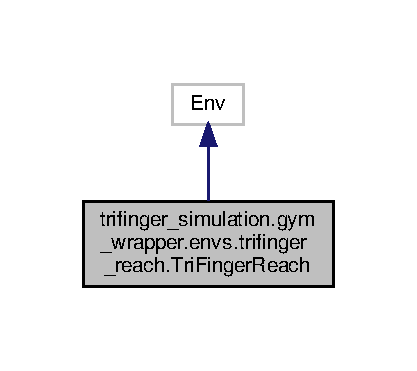
\includegraphics[width=200pt]{classtrifinger__simulation_1_1gym__wrapper_1_1envs_1_1trifinger__reach_1_1TriFingerReach__inherit__graph}
\end{center}
\end{figure}


Collaboration diagram for trifinger\+\_\+simulation.\+gym\+\_\+wrapper.\+envs.\+trifinger\+\_\+reach.\+Tri\+Finger\+Reach\+:
\nopagebreak
\begin{figure}[H]
\begin{center}
\leavevmode
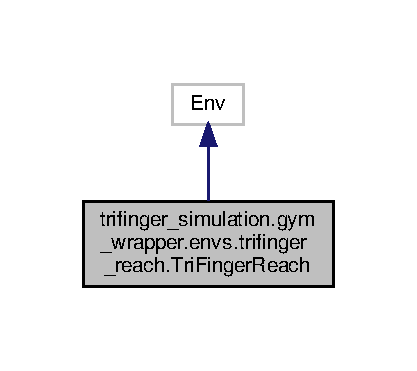
\includegraphics[width=200pt]{classtrifinger__simulation_1_1gym__wrapper_1_1envs_1_1trifinger__reach_1_1TriFingerReach__coll__graph}
\end{center}
\end{figure}
\subsection*{Public Member Functions}
\begin{DoxyCompactItemize}
\item 
def \hyperlink{classtrifinger__simulation_1_1gym__wrapper_1_1envs_1_1trifinger__reach_1_1TriFingerReach_afa5e38aa9079d1b271d291e3d197f423}{\+\_\+\+\_\+init\+\_\+\+\_\+} (self, control\+\_\+rate\+\_\+s, finger\+\_\+type, enable\+\_\+visualization, smoothing\+\_\+params, use\+\_\+real\+\_\+robot=False, finger\+\_\+config\+\_\+suffix=\char`\"{}0\char`\"{}, synchronize=False)
\begin{DoxyCompactList}\small\item\em Intializes the constituents of the reaching environment. \end{DoxyCompactList}\item 
def \hyperlink{classtrifinger__simulation_1_1gym__wrapper_1_1envs_1_1trifinger__reach_1_1TriFingerReach_a949ff008d719543f6146d276698bd9f1}{step} (self, action)
\begin{DoxyCompactList}\small\item\em The env step method. \end{DoxyCompactList}\item 
def \hyperlink{classtrifinger__simulation_1_1gym__wrapper_1_1envs_1_1trifinger__reach_1_1TriFingerReach_a46ae0ba9d5fc6cf4b8809db2fce2502b}{reset} (self)
\begin{DoxyCompactList}\small\item\em Episode reset. \end{DoxyCompactList}\item 
\mbox{\Hypertarget{classtrifinger__simulation_1_1gym__wrapper_1_1envs_1_1trifinger__reach_1_1TriFingerReach_ab09049dd0356e3c89a3145affbe9dcc7}\label{classtrifinger__simulation_1_1gym__wrapper_1_1envs_1_1trifinger__reach_1_1TriFingerReach_ab09049dd0356e3c89a3145affbe9dcc7}} 
def {\bfseries update\+\_\+smoothing} (self)
\end{DoxyCompactItemize}
\subsection*{Public Attributes}
\begin{DoxyCompactItemize}
\item 
\mbox{\Hypertarget{classtrifinger__simulation_1_1gym__wrapper_1_1envs_1_1trifinger__reach_1_1TriFingerReach_a40761207f831c145563063a8927b555a}\label{classtrifinger__simulation_1_1gym__wrapper_1_1envs_1_1trifinger__reach_1_1TriFingerReach_a40761207f831c145563063a8927b555a}} 
{\bfseries finger}
\item 
\mbox{\Hypertarget{classtrifinger__simulation_1_1gym__wrapper_1_1envs_1_1trifinger__reach_1_1TriFingerReach_a8664e4007a50193ac435376abe6c54d1}\label{classtrifinger__simulation_1_1gym__wrapper_1_1envs_1_1trifinger__reach_1_1TriFingerReach_a8664e4007a50193ac435376abe6c54d1}} 
{\bfseries num\+\_\+fingers}
\item 
\mbox{\Hypertarget{classtrifinger__simulation_1_1gym__wrapper_1_1envs_1_1trifinger__reach_1_1TriFingerReach_a627a8c4a6dc2815f85ba92e0f5387901}\label{classtrifinger__simulation_1_1gym__wrapper_1_1envs_1_1trifinger__reach_1_1TriFingerReach_a627a8c4a6dc2815f85ba92e0f5387901}} 
{\bfseries steps\+\_\+per\+\_\+control}
\item 
\mbox{\Hypertarget{classtrifinger__simulation_1_1gym__wrapper_1_1envs_1_1trifinger__reach_1_1TriFingerReach_ab750f136061b0b86d2fdde586836da4b}\label{classtrifinger__simulation_1_1gym__wrapper_1_1envs_1_1trifinger__reach_1_1TriFingerReach_ab750f136061b0b86d2fdde586836da4b}} 
{\bfseries observations\+\_\+keys}
\item 
\mbox{\Hypertarget{classtrifinger__simulation_1_1gym__wrapper_1_1envs_1_1trifinger__reach_1_1TriFingerReach_a9c48d4d5ceb1f5d0ce4818e0acb0a07a}\label{classtrifinger__simulation_1_1gym__wrapper_1_1envs_1_1trifinger__reach_1_1TriFingerReach_a9c48d4d5ceb1f5d0ce4818e0acb0a07a}} 
{\bfseries observations\+\_\+sizes}
\item 
\mbox{\Hypertarget{classtrifinger__simulation_1_1gym__wrapper_1_1envs_1_1trifinger__reach_1_1TriFingerReach_a6b8bb22fe0248fb4818cd62a61c8913c}\label{classtrifinger__simulation_1_1gym__wrapper_1_1envs_1_1trifinger__reach_1_1TriFingerReach_a6b8bb22fe0248fb4818cd62a61c8913c}} 
{\bfseries spaces}
\item 
\mbox{\Hypertarget{classtrifinger__simulation_1_1gym__wrapper_1_1envs_1_1trifinger__reach_1_1TriFingerReach_a77527a455bb41fc26b3b57d775035965}\label{classtrifinger__simulation_1_1gym__wrapper_1_1envs_1_1trifinger__reach_1_1TriFingerReach_a77527a455bb41fc26b3b57d775035965}} 
{\bfseries unscaled\+\_\+observation\+\_\+space}
\item 
\mbox{\Hypertarget{classtrifinger__simulation_1_1gym__wrapper_1_1envs_1_1trifinger__reach_1_1TriFingerReach_a6f2f28512cbebb6af3385b9fe8fb9b43}\label{classtrifinger__simulation_1_1gym__wrapper_1_1envs_1_1trifinger__reach_1_1TriFingerReach_a6f2f28512cbebb6af3385b9fe8fb9b43}} 
{\bfseries unscaled\+\_\+action\+\_\+space}
\item 
\mbox{\Hypertarget{classtrifinger__simulation_1_1gym__wrapper_1_1envs_1_1trifinger__reach_1_1TriFingerReach_a09a2283062675b043704578c6e210beb}\label{classtrifinger__simulation_1_1gym__wrapper_1_1envs_1_1trifinger__reach_1_1TriFingerReach_a09a2283062675b043704578c6e210beb}} 
{\bfseries observation\+\_\+space}
\item 
\mbox{\Hypertarget{classtrifinger__simulation_1_1gym__wrapper_1_1envs_1_1trifinger__reach_1_1TriFingerReach_ae21315a9d73e0eab522cade2a8ede91d}\label{classtrifinger__simulation_1_1gym__wrapper_1_1envs_1_1trifinger__reach_1_1TriFingerReach_ae21315a9d73e0eab522cade2a8ede91d}} 
{\bfseries action\+\_\+space}
\item 
\mbox{\Hypertarget{classtrifinger__simulation_1_1gym__wrapper_1_1envs_1_1trifinger__reach_1_1TriFingerReach_a3c54900b78139f63aee5ab4df9d15479}\label{classtrifinger__simulation_1_1gym__wrapper_1_1envs_1_1trifinger__reach_1_1TriFingerReach_a3c54900b78139f63aee5ab4df9d15479}} 
{\bfseries logger}
\item 
\mbox{\Hypertarget{classtrifinger__simulation_1_1gym__wrapper_1_1envs_1_1trifinger__reach_1_1TriFingerReach_ac9f2d2b95d2be69549a2e7009e97fe64}\label{classtrifinger__simulation_1_1gym__wrapper_1_1envs_1_1trifinger__reach_1_1TriFingerReach_ac9f2d2b95d2be69549a2e7009e97fe64}} 
{\bfseries smoothing\+\_\+start\+\_\+episode}
\item 
\mbox{\Hypertarget{classtrifinger__simulation_1_1gym__wrapper_1_1envs_1_1trifinger__reach_1_1TriFingerReach_a35109591538d36d6ba80faf3e7cf8213}\label{classtrifinger__simulation_1_1gym__wrapper_1_1envs_1_1trifinger__reach_1_1TriFingerReach_a35109591538d36d6ba80faf3e7cf8213}} 
{\bfseries smoothing\+\_\+alpha}
\item 
\mbox{\Hypertarget{classtrifinger__simulation_1_1gym__wrapper_1_1envs_1_1trifinger__reach_1_1TriFingerReach_ac3562e5bdc61f78d7d6a8ca395af4bc7}\label{classtrifinger__simulation_1_1gym__wrapper_1_1envs_1_1trifinger__reach_1_1TriFingerReach_ac3562e5bdc61f78d7d6a8ca395af4bc7}} 
{\bfseries smoothing\+\_\+increase\+\_\+step}
\item 
\mbox{\Hypertarget{classtrifinger__simulation_1_1gym__wrapper_1_1envs_1_1trifinger__reach_1_1TriFingerReach_ac4b1068fc50138a9ee0c43bf2a4c9083}\label{classtrifinger__simulation_1_1gym__wrapper_1_1envs_1_1trifinger__reach_1_1TriFingerReach_ac4b1068fc50138a9ee0c43bf2a4c9083}} 
{\bfseries smoothing\+\_\+stop\+\_\+episode}
\item 
\mbox{\Hypertarget{classtrifinger__simulation_1_1gym__wrapper_1_1envs_1_1trifinger__reach_1_1TriFingerReach_afa163934c0b3b563a52aacae2bfd4cc5}\label{classtrifinger__simulation_1_1gym__wrapper_1_1envs_1_1trifinger__reach_1_1TriFingerReach_afa163934c0b3b563a52aacae2bfd4cc5}} 
{\bfseries smoothed\+\_\+action}
\item 
\mbox{\Hypertarget{classtrifinger__simulation_1_1gym__wrapper_1_1envs_1_1trifinger__reach_1_1TriFingerReach_a6449c7054118a4a2369a31f4e604f8ca}\label{classtrifinger__simulation_1_1gym__wrapper_1_1envs_1_1trifinger__reach_1_1TriFingerReach_a6449c7054118a4a2369a31f4e604f8ca}} 
{\bfseries episode\+\_\+count}
\item 
\mbox{\Hypertarget{classtrifinger__simulation_1_1gym__wrapper_1_1envs_1_1trifinger__reach_1_1TriFingerReach_a59bda8f623fbc8c7fe4a52c00ceec355}\label{classtrifinger__simulation_1_1gym__wrapper_1_1envs_1_1trifinger__reach_1_1TriFingerReach_a59bda8f623fbc8c7fe4a52c00ceec355}} 
{\bfseries enable\+\_\+visualization}
\item 
\mbox{\Hypertarget{classtrifinger__simulation_1_1gym__wrapper_1_1envs_1_1trifinger__reach_1_1TriFingerReach_a9ac1cec7a60d3e1d6ef4408e664534a6}\label{classtrifinger__simulation_1_1gym__wrapper_1_1envs_1_1trifinger__reach_1_1TriFingerReach_a9ac1cec7a60d3e1d6ef4408e664534a6}} 
{\bfseries goal\+\_\+marker}
\item 
\mbox{\Hypertarget{classtrifinger__simulation_1_1gym__wrapper_1_1envs_1_1trifinger__reach_1_1TriFingerReach_aee1978105a61ffa44910ba2e9b04319c}\label{classtrifinger__simulation_1_1gym__wrapper_1_1envs_1_1trifinger__reach_1_1TriFingerReach_aee1978105a61ffa44910ba2e9b04319c}} 
{\bfseries synchronize}
\item 
\mbox{\Hypertarget{classtrifinger__simulation_1_1gym__wrapper_1_1envs_1_1trifinger__reach_1_1TriFingerReach_a07c7a02b99238a296eaacee933703c85}\label{classtrifinger__simulation_1_1gym__wrapper_1_1envs_1_1trifinger__reach_1_1TriFingerReach_a07c7a02b99238a296eaacee933703c85}} 
{\bfseries next\+\_\+start\+\_\+time}
\item 
\mbox{\Hypertarget{classtrifinger__simulation_1_1gym__wrapper_1_1envs_1_1trifinger__reach_1_1TriFingerReach_a9fc715670f8555e836694a118fc54441}\label{classtrifinger__simulation_1_1gym__wrapper_1_1envs_1_1trifinger__reach_1_1TriFingerReach_a9fc715670f8555e836694a118fc54441}} 
{\bfseries observation}
\item 
\mbox{\Hypertarget{classtrifinger__simulation_1_1gym__wrapper_1_1envs_1_1trifinger__reach_1_1TriFingerReach_a886d8b46fed911730f1e31d00435cd38}\label{classtrifinger__simulation_1_1gym__wrapper_1_1envs_1_1trifinger__reach_1_1TriFingerReach_a886d8b46fed911730f1e31d00435cd38}} 
{\bfseries goal}
\end{DoxyCompactItemize}
\subsection*{Private Member Functions}
\begin{DoxyCompactItemize}
\item 
def \hyperlink{classtrifinger__simulation_1_1gym__wrapper_1_1envs_1_1trifinger__reach_1_1TriFingerReach_a05a8368ada911496c2b2e582aac976da}{\+\_\+compute\+\_\+reward} (self, observation, goal)
\begin{DoxyCompactList}\small\item\em The reward function of the environment. \end{DoxyCompactList}\item 
def \hyperlink{classtrifinger__simulation_1_1gym__wrapper_1_1envs_1_1trifinger__reach_1_1TriFingerReach_a1aab2e39d91a3fba25437b8497972460}{\+\_\+get\+\_\+state} (self, observation, action, log\+\_\+observation=False)
\begin{DoxyCompactList}\small\item\em Get the current observation from the env for the agent. \end{DoxyCompactList}\end{DoxyCompactItemize}


\subsection{Constructor \& Destructor Documentation}
\mbox{\Hypertarget{classtrifinger__simulation_1_1gym__wrapper_1_1envs_1_1trifinger__reach_1_1TriFingerReach_afa5e38aa9079d1b271d291e3d197f423}\label{classtrifinger__simulation_1_1gym__wrapper_1_1envs_1_1trifinger__reach_1_1TriFingerReach_afa5e38aa9079d1b271d291e3d197f423}} 
\index{trifinger\+\_\+simulation\+::gym\+\_\+wrapper\+::envs\+::trifinger\+\_\+reach\+::\+Tri\+Finger\+Reach@{trifinger\+\_\+simulation\+::gym\+\_\+wrapper\+::envs\+::trifinger\+\_\+reach\+::\+Tri\+Finger\+Reach}!\+\_\+\+\_\+init\+\_\+\+\_\+@{\+\_\+\+\_\+init\+\_\+\+\_\+}}
\index{\+\_\+\+\_\+init\+\_\+\+\_\+@{\+\_\+\+\_\+init\+\_\+\+\_\+}!trifinger\+\_\+simulation\+::gym\+\_\+wrapper\+::envs\+::trifinger\+\_\+reach\+::\+Tri\+Finger\+Reach@{trifinger\+\_\+simulation\+::gym\+\_\+wrapper\+::envs\+::trifinger\+\_\+reach\+::\+Tri\+Finger\+Reach}}
\subsubsection{\texorpdfstring{\+\_\+\+\_\+init\+\_\+\+\_\+()}{\_\_init\_\_()}}
{\footnotesize\ttfamily def trifinger\+\_\+simulation.\+gym\+\_\+wrapper.\+envs.\+trifinger\+\_\+reach.\+Tri\+Finger\+Reach.\+\_\+\+\_\+init\+\_\+\+\_\+ (\begin{DoxyParamCaption}\item[{}]{self,  }\item[{}]{control\+\_\+rate\+\_\+s,  }\item[{}]{finger\+\_\+type,  }\item[{}]{enable\+\_\+visualization,  }\item[{}]{smoothing\+\_\+params,  }\item[{}]{use\+\_\+real\+\_\+robot = {\ttfamily False},  }\item[{}]{finger\+\_\+config\+\_\+suffix = {\ttfamily \char`\"{}0\char`\"{}},  }\item[{}]{synchronize = {\ttfamily False} }\end{DoxyParamCaption})}



Intializes the constituents of the reaching environment. 

Constructor sets up the finger robot depending on the finger type, and also whether an instance of the simulated or the real robot is to be created. Also sets up the observation and action spaces, smoothing for reducing jitter on the robot, and provides for a way to synchronize robots being trained independently.


\begin{DoxyParams}{Parameters}
{\em control\+\_\+rate\+\_\+s} & the rate (in seconds) at which step method of the env will run. The actual robot controller may run at a higher rate, so this is used to compute the number of robot control updates per environment step. \\
\hline
{\em finger\+\_\+type} & Name of the finger type. In order to get a dictionary of the valid finger types, call \+:meth\+:{\ttfamily .finger\+\_\+types\+\_\+data.\+get\+\_\+valid\+\_\+finger\+\_\+types} \\
\hline
{\em enable\+\_\+visualization} & if the simulation env is to be \\
\hline
{\em visualized} & smoothing\+\_\+params (dict)\+: \\
\hline
{\em num\+\_\+episodes} & the total number of episodes for which the 
\begin{DoxyCode}
                   training \textcolor{keywordflow}{is} performed
@param     start\_after the fraction of episodes after which the
\end{DoxyCode}
 smoothing of applied actions to the motors should start \\
\hline
{\em final\+\_\+alpha} & smoothing coeff that will be reached at the end of the smoothing \\
\hline
{\em stop\+\_\+after} & the fraction of total episodes by which final alpha is to be reached, after which the same final alpha will be used for smoothing in the remainder of the episodes is\+\_\+test (bool, optional)\+: Include this for testing \\
\hline
{\em use\+\_\+real\+\_\+robot} & if training is to be performed on the real robot (\mbox{[}default\mbox{]} False) \\
\hline
{\em finger\+\_\+config\+\_\+suffix} & pass this if only one of the three fingers is to be trained. Valid choices include \mbox{[}0, 120, 240\mbox{]} (\mbox{[}default\mbox{]} 0) \\
\hline
{\em synchronize} & Set this to True if you want to train independently on three fingers in separate processes, but have them synchronized. (\mbox{[}default\mbox{]} False) \\
\hline
\end{DoxyParams}


\subsection{Member Function Documentation}
\mbox{\Hypertarget{classtrifinger__simulation_1_1gym__wrapper_1_1envs_1_1trifinger__reach_1_1TriFingerReach_a05a8368ada911496c2b2e582aac976da}\label{classtrifinger__simulation_1_1gym__wrapper_1_1envs_1_1trifinger__reach_1_1TriFingerReach_a05a8368ada911496c2b2e582aac976da}} 
\index{trifinger\+\_\+simulation\+::gym\+\_\+wrapper\+::envs\+::trifinger\+\_\+reach\+::\+Tri\+Finger\+Reach@{trifinger\+\_\+simulation\+::gym\+\_\+wrapper\+::envs\+::trifinger\+\_\+reach\+::\+Tri\+Finger\+Reach}!\+\_\+compute\+\_\+reward@{\+\_\+compute\+\_\+reward}}
\index{\+\_\+compute\+\_\+reward@{\+\_\+compute\+\_\+reward}!trifinger\+\_\+simulation\+::gym\+\_\+wrapper\+::envs\+::trifinger\+\_\+reach\+::\+Tri\+Finger\+Reach@{trifinger\+\_\+simulation\+::gym\+\_\+wrapper\+::envs\+::trifinger\+\_\+reach\+::\+Tri\+Finger\+Reach}}
\subsubsection{\texorpdfstring{\+\_\+compute\+\_\+reward()}{\_compute\_reward()}}
{\footnotesize\ttfamily def trifinger\+\_\+simulation.\+gym\+\_\+wrapper.\+envs.\+trifinger\+\_\+reach.\+Tri\+Finger\+Reach.\+\_\+compute\+\_\+reward (\begin{DoxyParamCaption}\item[{}]{self,  }\item[{}]{observation,  }\item[{}]{goal }\end{DoxyParamCaption})\hspace{0.3cm}{\ttfamily [private]}}



The reward function of the environment. 


\begin{DoxyParams}{Parameters}
{\em observation} & the observation at the current step \\
\hline
{\em goal} & the desired goal for the episode\\
\hline
\end{DoxyParams}
\begin{DoxyReturn}{Returns}
the reward, and the done signal 
\end{DoxyReturn}
\mbox{\Hypertarget{classtrifinger__simulation_1_1gym__wrapper_1_1envs_1_1trifinger__reach_1_1TriFingerReach_a1aab2e39d91a3fba25437b8497972460}\label{classtrifinger__simulation_1_1gym__wrapper_1_1envs_1_1trifinger__reach_1_1TriFingerReach_a1aab2e39d91a3fba25437b8497972460}} 
\index{trifinger\+\_\+simulation\+::gym\+\_\+wrapper\+::envs\+::trifinger\+\_\+reach\+::\+Tri\+Finger\+Reach@{trifinger\+\_\+simulation\+::gym\+\_\+wrapper\+::envs\+::trifinger\+\_\+reach\+::\+Tri\+Finger\+Reach}!\+\_\+get\+\_\+state@{\+\_\+get\+\_\+state}}
\index{\+\_\+get\+\_\+state@{\+\_\+get\+\_\+state}!trifinger\+\_\+simulation\+::gym\+\_\+wrapper\+::envs\+::trifinger\+\_\+reach\+::\+Tri\+Finger\+Reach@{trifinger\+\_\+simulation\+::gym\+\_\+wrapper\+::envs\+::trifinger\+\_\+reach\+::\+Tri\+Finger\+Reach}}
\subsubsection{\texorpdfstring{\+\_\+get\+\_\+state()}{\_get\_state()}}
{\footnotesize\ttfamily def trifinger\+\_\+simulation.\+gym\+\_\+wrapper.\+envs.\+trifinger\+\_\+reach.\+Tri\+Finger\+Reach.\+\_\+get\+\_\+state (\begin{DoxyParamCaption}\item[{}]{self,  }\item[{}]{observation,  }\item[{}]{action,  }\item[{}]{log\+\_\+observation = {\ttfamily False} }\end{DoxyParamCaption})\hspace{0.3cm}{\ttfamily [private]}}



Get the current observation from the env for the agent. 


\begin{DoxyParams}{Parameters}
{\em log\+\_\+observation} & specify whether you want to log the observation\\
\hline
\end{DoxyParams}
\begin{DoxyReturn}{Returns}


observation comprising of the observations corresponding to the key values in the observation\+\_\+keys 
\end{DoxyReturn}
\mbox{\Hypertarget{classtrifinger__simulation_1_1gym__wrapper_1_1envs_1_1trifinger__reach_1_1TriFingerReach_a46ae0ba9d5fc6cf4b8809db2fce2502b}\label{classtrifinger__simulation_1_1gym__wrapper_1_1envs_1_1trifinger__reach_1_1TriFingerReach_a46ae0ba9d5fc6cf4b8809db2fce2502b}} 
\index{trifinger\+\_\+simulation\+::gym\+\_\+wrapper\+::envs\+::trifinger\+\_\+reach\+::\+Tri\+Finger\+Reach@{trifinger\+\_\+simulation\+::gym\+\_\+wrapper\+::envs\+::trifinger\+\_\+reach\+::\+Tri\+Finger\+Reach}!reset@{reset}}
\index{reset@{reset}!trifinger\+\_\+simulation\+::gym\+\_\+wrapper\+::envs\+::trifinger\+\_\+reach\+::\+Tri\+Finger\+Reach@{trifinger\+\_\+simulation\+::gym\+\_\+wrapper\+::envs\+::trifinger\+\_\+reach\+::\+Tri\+Finger\+Reach}}
\subsubsection{\texorpdfstring{reset()}{reset()}}
{\footnotesize\ttfamily def trifinger\+\_\+simulation.\+gym\+\_\+wrapper.\+envs.\+trifinger\+\_\+reach.\+Tri\+Finger\+Reach.\+reset (\begin{DoxyParamCaption}\item[{}]{self }\end{DoxyParamCaption})}



Episode reset. 

\begin{DoxyReturn}{Returns}
the scaled to \mbox{[}-\/1;1\mbox{]} observation from the env after the reset 
\end{DoxyReturn}
\mbox{\Hypertarget{classtrifinger__simulation_1_1gym__wrapper_1_1envs_1_1trifinger__reach_1_1TriFingerReach_a949ff008d719543f6146d276698bd9f1}\label{classtrifinger__simulation_1_1gym__wrapper_1_1envs_1_1trifinger__reach_1_1TriFingerReach_a949ff008d719543f6146d276698bd9f1}} 
\index{trifinger\+\_\+simulation\+::gym\+\_\+wrapper\+::envs\+::trifinger\+\_\+reach\+::\+Tri\+Finger\+Reach@{trifinger\+\_\+simulation\+::gym\+\_\+wrapper\+::envs\+::trifinger\+\_\+reach\+::\+Tri\+Finger\+Reach}!step@{step}}
\index{step@{step}!trifinger\+\_\+simulation\+::gym\+\_\+wrapper\+::envs\+::trifinger\+\_\+reach\+::\+Tri\+Finger\+Reach@{trifinger\+\_\+simulation\+::gym\+\_\+wrapper\+::envs\+::trifinger\+\_\+reach\+::\+Tri\+Finger\+Reach}}
\subsubsection{\texorpdfstring{step()}{step()}}
{\footnotesize\ttfamily def trifinger\+\_\+simulation.\+gym\+\_\+wrapper.\+envs.\+trifinger\+\_\+reach.\+Tri\+Finger\+Reach.\+step (\begin{DoxyParamCaption}\item[{}]{self,  }\item[{}]{action }\end{DoxyParamCaption})}



The env step method. 


\begin{DoxyParams}{Parameters}
{\em action} & the joint positions that have to be achieved\\
\hline
\end{DoxyParams}
\begin{DoxyReturn}{Returns}
the observation scaled to lie between \mbox{[}-\/1;1\mbox{]}, the reward, the done signal, and info on if the agent was successful at the current step 
\end{DoxyReturn}


The documentation for this class was generated from the following file\+:\begin{DoxyCompactItemize}
\item 
python/trifinger\+\_\+simulation/gym\+\_\+wrapper/envs/trifinger\+\_\+reach.\+py\end{DoxyCompactItemize}

\chapter{File Documentation}
\hypertarget{pybullet__driver_8hpp}{}\section{include/trifinger\+\_\+simulation/pybullet\+\_\+driver.hpp File Reference}
\label{pybullet__driver_8hpp}\index{include/trifinger\+\_\+simulation/pybullet\+\_\+driver.\+hpp@{include/trifinger\+\_\+simulation/pybullet\+\_\+driver.\+hpp}}


C++ wrappers to use py\+Bullet simulation of fingers as robot\+\_\+interfaces\+::\+Robot\+Driver.  


{\ttfamily \#include $<$chrono$>$}\newline
{\ttfamily \#include $<$thread$>$}\newline
{\ttfamily \#include $<$pybind11/eigen.\+h$>$}\newline
{\ttfamily \#include $<$pybind11/embed.\+h$>$}\newline
{\ttfamily \#include $<$robot\+\_\+interfaces/finger\+\_\+types.\+hpp$>$}\newline
Include dependency graph for pybullet\+\_\+driver.\+hpp\+:
\nopagebreak
\begin{figure}[H]
\begin{center}
\leavevmode
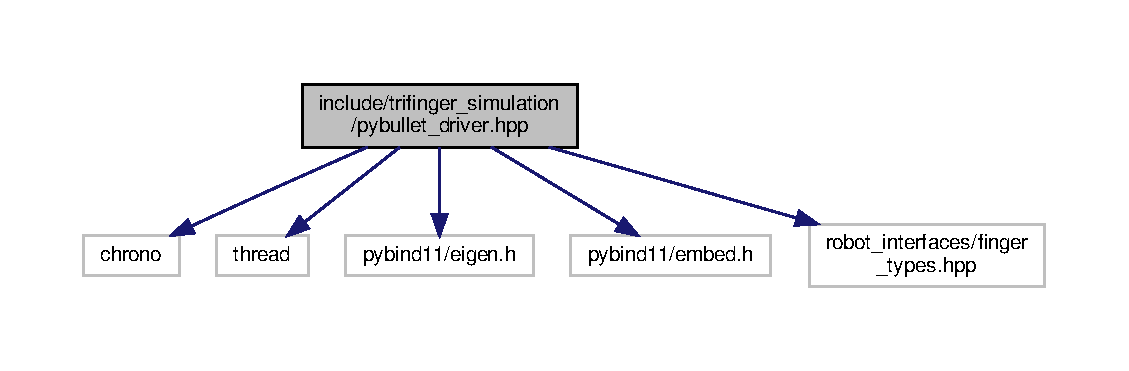
\includegraphics[width=350pt]{pybullet__driver_8hpp__incl}
\end{center}
\end{figure}
\subsection*{Classes}
\begin{DoxyCompactItemize}
\item 
class \hyperlink{classtrifinger__simulation_1_1BasePyBulletFingerDriver}{trifinger\+\_\+simulation\+::\+Base\+Py\+Bullet\+Finger\+Driver$<$ Action, Observation $>$}
\begin{DoxyCompactList}\small\item\em Base driver for py\+Bullet of both single Finger and Tri\+Finger. \end{DoxyCompactList}\item 
class \hyperlink{classtrifinger__simulation_1_1PyBulletSingleFingerDriver}{trifinger\+\_\+simulation\+::\+Py\+Bullet\+Single\+Finger\+Driver}
\begin{DoxyCompactList}\small\item\em py\+Bullet driver for the single Finger. \end{DoxyCompactList}\item 
class \hyperlink{classtrifinger__simulation_1_1PyBulletTriFingerDriver}{trifinger\+\_\+simulation\+::\+Py\+Bullet\+Tri\+Finger\+Driver}
\begin{DoxyCompactList}\small\item\em py\+Bullet driver for the Tri\+Finger \end{DoxyCompactList}\end{DoxyCompactItemize}
\subsection*{Functions}
\begin{DoxyCompactItemize}
\item 
{\footnotesize template$<$typename Types , typename Driver $>$ }\\Types\+::\+Backend\+Ptr \hyperlink{pybullet__driver_8hpp_a41d03263393c283e44ad605b4acc0d8b}{trifinger\+\_\+simulation\+::create\+\_\+finger\+\_\+backend} (typename Types\+::\+Base\+Data\+Ptr robot\+\_\+data, const bool real\+\_\+time\+\_\+mode, const bool visualize, const double first\+\_\+action\+\_\+timeout=std\+::numeric\+\_\+limits$<$ double $>$\+::infinity(), const uint32\+\_\+t max\+\_\+number\+\_\+of\+\_\+actions=0)
\begin{DoxyCompactList}\small\item\em Create a Finger/\+Tri\+Finger-\/backend using py\+Bullet. \end{DoxyCompactList}\end{DoxyCompactItemize}


\subsection{Detailed Description}
C++ wrappers to use py\+Bullet simulation of fingers as robot\+\_\+interfaces\+::\+Robot\+Driver. 



\subsection{Function Documentation}
\mbox{\Hypertarget{pybullet__driver_8hpp_file_a41d03263393c283e44ad605b4acc0d8b}\label{pybullet__driver_8hpp_file_a41d03263393c283e44ad605b4acc0d8b}} 
\index{pybullet\+\_\+driver.\+hpp@{pybullet\+\_\+driver.\+hpp}!create\+\_\+finger\+\_\+backend@{create\+\_\+finger\+\_\+backend}}
\index{create\+\_\+finger\+\_\+backend@{create\+\_\+finger\+\_\+backend}!pybullet\+\_\+driver.\+hpp@{pybullet\+\_\+driver.\+hpp}}
\subsubsection{\texorpdfstring{create\+\_\+finger\+\_\+backend()}{create\_finger\_backend()}}
{\footnotesize\ttfamily template$<$typename Types , typename Driver $>$ \\
Types\+::\+Backend\+Ptr trifinger\+\_\+simulation\+::create\+\_\+finger\+\_\+backend (\begin{DoxyParamCaption}\item[{typename Types\+::\+Base\+Data\+Ptr}]{robot\+\_\+data,  }\item[{const bool}]{real\+\_\+time\+\_\+mode,  }\item[{const bool}]{visualize,  }\item[{const double}]{first\+\_\+action\+\_\+timeout = {\ttfamily std\+:\+:numeric\+\_\+limits$<$double$>$\+:\+:infinity()},  }\item[{const uint32\+\_\+t}]{max\+\_\+number\+\_\+of\+\_\+actions = {\ttfamily 0} }\end{DoxyParamCaption})}



Create a Finger/\+Tri\+Finger-\/backend using py\+Bullet. 


\begin{DoxyTemplParams}{Template Parameters}
{\em Types} & The struct providing the types for action, observation, etc. \\
\hline
{\em Driver} & py\+Bullet-\/\+Driver class for either single Finger or Tri\+Finger.\\
\hline
\end{DoxyTemplParams}

\begin{DoxyParams}{Parameters}
{\em robot\+\_\+data} & Robot\+Data instance for the backend. \\
\hline
{\em real\+\_\+time\+\_\+mode} & If true, step the simulation in real time, otherwise as fast as possible. \\
\hline
{\em visualize} & If true, py\+Bullet\textquotesingle{}s G\+UI is started for visualization. \\
\hline
{\em first\+\_\+action\+\_\+timeout} & See Robot\+Backend \\
\hline
{\em max\+\_\+number\+\_\+of\+\_\+actions} & See Robot\+Backend\\
\hline
\end{DoxyParams}
\begin{DoxyReturn}{Returns}
Backend using a driver of the specified type. 
\end{DoxyReturn}

%--- End generated contents ---

% Index
\backmatter
\newpage
\phantomsection
\clearemptydoublepage
\addcontentsline{toc}{chapter}{Index}
\printindex

\end{document}
